\PassOptionsToPackage{hyphens}{url}
\PassOptionsToPackage{pdftex,dvipsnames}{xcolor}
\documentclass[11pt,oneside,openright]{mpreport}
\usepackage[type=master]{wdok-title}
\usepackage[utf8]{inputenc}
\usepackage[T1]{fontenc}
\usepackage[ngerman,english]{babel}
\usepackage{textcomp}
\usepackage{mathptmx}
\usepackage[scaled=0.9]{helvet}
\usepackage{courier}
\usepackage[hidelinks]{hyperref}
\usepackage{cleveref}
\usepackage{siunitx}
\usepackage{listings}
\usepackage[bibencoding=auto,backend=biber,autolang=other]{biblatex}
\usepackage{csquotes}
\usepackage{amssymb}
%\usepackage[style=numeric]{biblatex}
\addbibresource{main.bib}
\usepackage{mathtools}
\usepackage{svg}
\usepackage{tikz}


\usepackage{tikz-uml}
\usepackage{pgfplots}
\pgfplotsset{compat=1.14}
\usepackage{xargs}                      % Use more than one optional parameter in a new commands
\usepackage{acronym}
\usepackage{tabularx}
\usepackage{subcaption}

\newbibmacro*{bbx:parunit}{%
  \ifbibliography
    {\setunit{\bibpagerefpunct}\newblock
     \usebibmacro{pageref}%
     \clearlist{pageref}%
     \setunit{\adddot\par\nobreak}}
    {}}

\renewbibmacro*{doi+eprint+url}{%
  \usebibmacro{bbx:parunit}% Added
  \iftoggle{bbx:doi}
    {\printfield{doi}}
    {}%
  \iftoggle{bbx:eprint}
    {\usebibmacro{eprint}}
    {}%
  \iftoggle{bbx:url}
    {\usebibmacro{url+urldate}}
    {}}

\renewbibmacro*{eprint}{%
  \usebibmacro{bbx:parunit}% Added
  \iffieldundef{eprinttype}
    {\printfield{eprint}}
    {\printfield[eprint:\strfield{eprinttype}]{eprint}}}

\renewbibmacro*{url+urldate}{%
  \usebibmacro{bbx:parunit}% Added
  \printfield{url}%
  \iffieldundef{urlyear}
    {}
    {\setunit*{\addspace}%
     \printtext[urldate]{\printurldate}}}


\setcounter{biburlnumpenalty}{100}  % allow breaks at numbers
\setcounter{biburlucpenalty}{100}   % allow breaks at uppercase letters
\setcounter{biburllcpenalty}{100}   % allow breaks at lowercase letters

\usepackage[colorinlistoftodos,prependcaption,textsize=tiny]{todonotes}
\newcommandx{\unsure}[2][1=]{\todo[linecolor=red,backgroundcolor=red!25,bordercolor=red,#1]{#2}}
\newcommandx{\change}[2][1=]{\todo[linecolor=blue,backgroundcolor=blue!25,bordercolor=blue,#1]{#2}}
\newcommandx{\info}[2][1=]{\todo[linecolor=OliveGreen,backgroundcolor=OliveGreen!25,bordercolor=OliveGreen,#1]{#2}}
\newcommandx{\improvement}[2][1=]{\todo[linecolor=Plum,backgroundcolor=Plum!25,bordercolor=Plum,#1]{#2}}
\newcommandx{\thiswillnotshow}[2][1=]{\todo[disable,#1]{#2}}

\DeclareMathOperator{\atantwo}{atan2}

% Examples for the definition of convenience commands
\newcommand{\package}[1]{\texttt{#1}}
\newcommand{\foreign}[1]{\emph{#1}}
\newcommand{\q}[1]{»#1«}


\newtheorem{defi}{Definition}[chapter]
\newtheorem{satz}{Satz}[chapter]
\newtheorem{bsp}{Beispiel}[chapter]

% Title Page
\title{Autonomous Driving in Urban Centers - Roundabout Monitoring}
\author{Julian-B. Scholle}

%\supervisor{Themensteller\\
%  Betreuer}

\pagenumbering{Roman}



\begin{document}

\maketitle



\chapter*{Eidesstattliche Erklärung}
Ich erkläre hiermit an Eides statt, dass ich die vorliegende Arbeit selbständig und
ohne unerlaubte fremde Hilfe angefertigt, andere als die angegebenen Quellen und
Hilfsmittel nicht benutzt habe. Die aus fremden Quellen direkt oder indirekt
übernommenen Stellen sind als solche kenntlich gemacht.
Die Arbeit wurde bisher in gleicher oder ähnlicher Form keinem anderen
Prüfungsamt vorgelegt und auch nicht veröffentlicht.

\noindent Göteborg, den \today
\begin{flushright}
$\overline{~~~~~~~~~\mbox{Julian-B. Scholle}~~~~~~~~~}$
\end{flushright}


\chapter*{Acknowledgements}
% Danken möchte ich außerdem besonders Associate professor Christian Berger und J. Prof Sebastian Zug, führ ihre Organisatorische und Fachliche Unterstützung während und besonders im Vorfeld dieser Arbeit und
% dem ``Deutschen Akademischen Austauschdienst'' - DAAD für ihre finanzielle Unterstüzung während meines Aufenthaltes in Göteborg.
% Weiterhin danken möchte ich natürlich allen weiteren Kollegen aus Götborg, welche mich bei meiner Arbeit fachlich und moralisch untersützt haben.

I would especially like to thank Associate Professor Christian Berger and J. Professor Sebastian Zug for their organizational and technical support during and especially in the run-up to this work and
the ``Deutschen Akademischen Austauschdienst'' - DAAD for their financial support during my stay in Gothenburg.
I would also like to thank all the other colleagues from Gothenburg, who have supported me professionally and morally.


\chapter*{Index of Abbreviations}

\begin{acronym}[Bash]
 \acro{DBSCAN} {Density-Based Spatial Clustering of Applications with Noise}
 \acro{SVD}{Singular Value Decomposition}
 \acro{LLSQ}{Linear least Squares}
 \acro{RANSAC}{Random Sample Consensus}
 \acro{MKS}{multi-body simulation}
 \acro{ACC}{Adaptive Cruise Control}
 \end{acronym}

\tableofcontents
\clearpage 

\pagenumbering{arabic}

\chapter{Introduction}

\todo{bezug auf kreisverkehre fehlt}

Das autonome Fahren und die Vernetzung von Fahrzeugen mit Ihrer Umwelt sind zusammen mit der Elektromobilität die meistdiskutierten Themen der Automobilbranche.
Zu Recht: Autonomes Fahren besitzt das Potenzial, im Mobilitätsmarkt völlig neue Strukturen entstehen zu lassen.
\footnote{\url{https://www2.deloitte.com/de/de/pages/consumer-industrial-products/articles/autonomes-fahren-in-deutschland.html} (03/09/2017)}

So ebenfalls die Technische Hochschule Chalmers welche ergänzend zu Volvos “DriveMe” Projekt das Projekt
“CampusShuttle” initiiert hat, “CampusShuttle” ist ein interdisziplinäres Forschungsprojekt der Technischen Hochschule Chalmers und der Universität Göteborg.
Das Projekt ist dabei im ReVeRe (Chalmers Research Vehicle Resource) angesiedelt. Die Vision ist dabei ein selbstfahrendes Auto zwischen den beiden Campus der Technische Hochschule Chalmers.

Dabei soll, im Rahmen des Projekts, das Fahrzeug in verschiedenen Verkehrsszenarien untersucht werden. Der Fokus liegt dabei besonders auf den Stadtverkehr, das Fahrzeug muss dabei nicht
nur in der Lage sein mit anderen Autos zu interagieren, sondern ebenfalls mit Straßenbahnen, Bussen, Fahrrädern aund allen Anderen Verkehrsteilnehmern sicher agieren. 

\section{Ausgangssituation}


\subsection{Test Platform}

\begin{figure}[!ht]
%\begin{center}
\caption{Test Platform Snowfox}
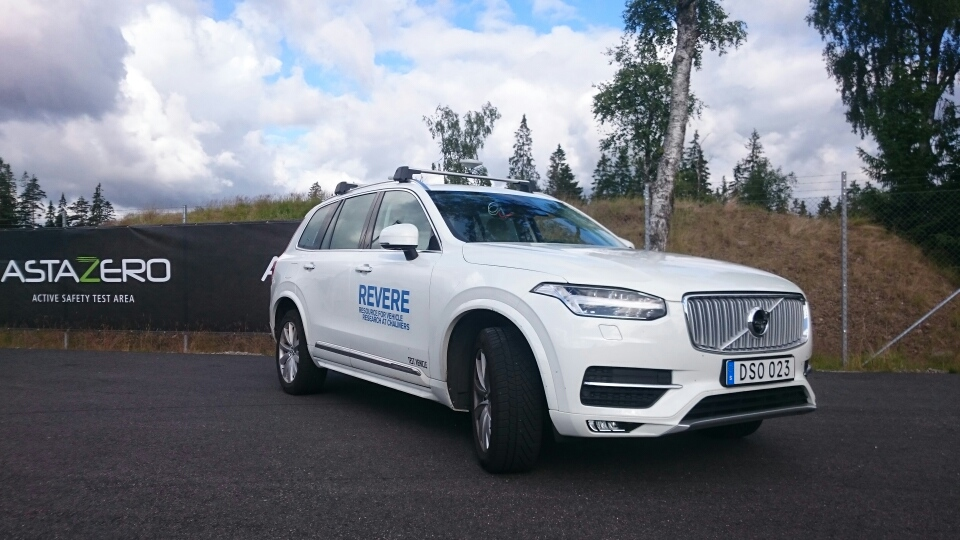
\includegraphics[width=\columnwidth]{bilder/snowfox.jpg}
\label{snowfox}
%\end{center}
\end{figure}

Die in dieser Arbeit genutze Testplatform ist ein Volvo XC90 (2015) SUV, gennate Snowfox (siehe \cref{snowfox}). Diese Testpaltform ist mit vielen Sensoren zur Umfeldwarnehmung ausgestattet.
Dazu zählen fünf Radar Sensoren, rund um das Fahrzeug. Wobei das Front Radar über eine Größere Reichweite verfügt. Sowie eine
Stereo Kamera und ein Velodyne VLP-16 LiDAR. Die Anordnung der Sensoren kann \cref{platform} entnommen werden.


\begin{figure}[!ht]
%\begin{center}
\caption{Snowfox Sensors}
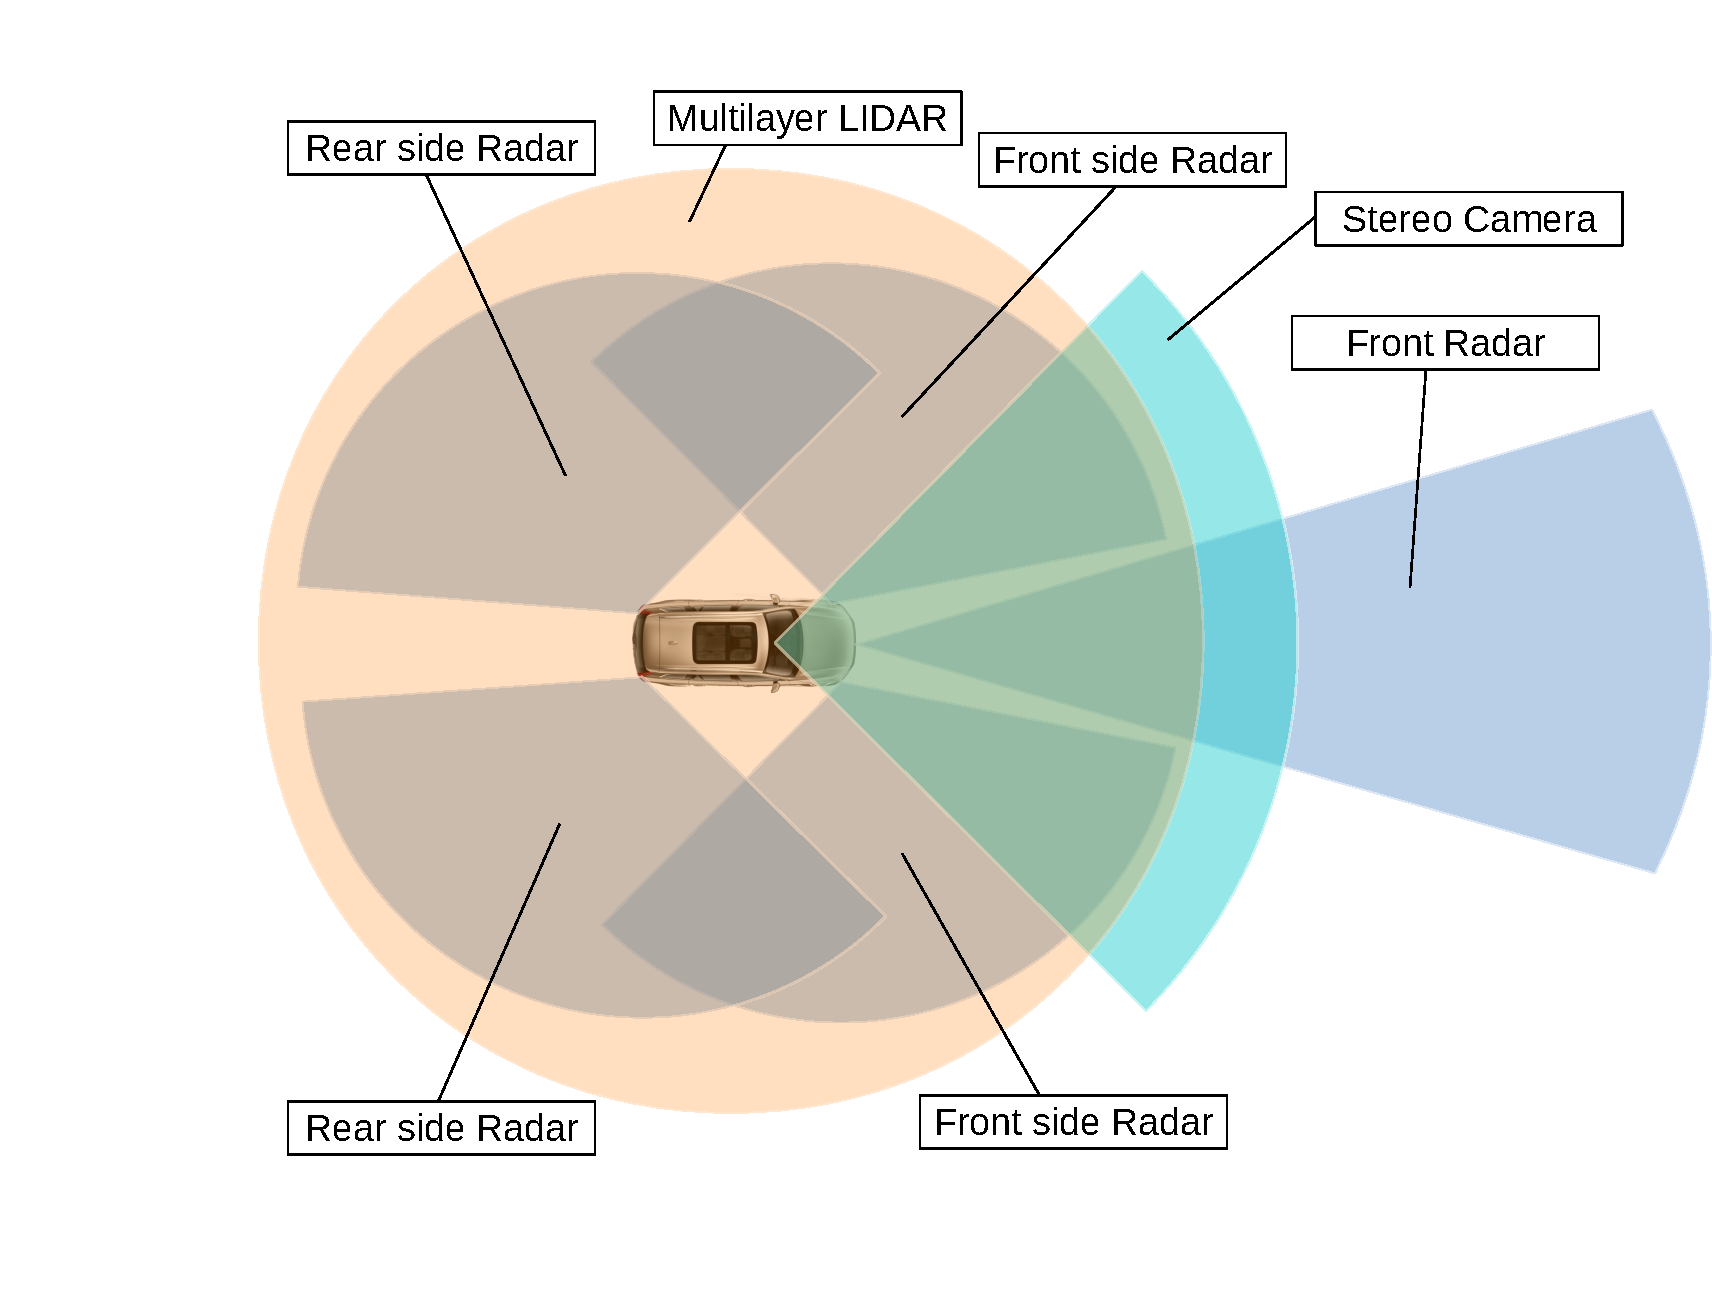
\includegraphics[width=\columnwidth]{sensors.pdf}
\label{platform}
%\end{center}
\end{figure}


Zusätlich zur Serienmäßgigen Fahrzeugsensorik (z.B. Odometer, Interialsensorik) ist im Fahrzeug ein Applanix POS LV verbaut. Zu Zeitpunkt des Verfassens dieser Arbeit war es leider noch nicht möglich auf
die Radarsensoren und die Stereokamera zuzugreifen. Daher werden im folgenden lediglich der Velodyne Lidar und das Applanix System genauer beschrieben.

\subsubsection{Velodyne VLP-16 LiDAR}
\todo{reichweitenanalyse (layer objet mit enbtfernung)}
Der Velodyne VLP-16 ist ein 360 Grad 3D Laserscannermit einer Rotationsgeschwindigkeit von 5 bis 20 Umdrehungen pro Sekunde \cite{manVEL}. Er bietet ein vertikales FOV von 30 Grad, bei 2 Grad Auflösung.
Mit einer Reichweite von 100m kann er einen Umkreis von 200m Durchmesser abdecken. Weiterhin kann der VLP-16 mit dem Applanix POS LV syncronisiert werden, was eine jitterarme Zeimessung ermöglicht.
Eine weiter Funktion des Velodyne Sensors, ist das er auf verschiedene Messimpulse reagieren kann. Durch die Auswertung des letzten Impulses statt des Stärksten Impulses ist es Möglich durch Transparent Objekte zu sehen.
Das ermöglicht uns im späteren Verlauf die Breite des Fahrzeues zu ermitteln, da der Velodyne durch die Glasfenster des Fahrzeues blicken kann.
Bei einer eingestellten Geschwindigkeit von 10Hz liefert der VLP-16 eine Auflösung von 0.2 Grad bei einer Abreichung von +-3cm. Der VLP-16 ist mittig auf dem Dach des XC90 moniert, um eine möglichst hohe Positionierung
zu erreichen, die eine Rundumsicht umd Das Fahrzeug zu erreichen. Zu beachten ist, das diese Ausrichtung für den Sensor denkbar ungünstig ist, da der Sensor ein vertikales
Sichtfeld von -15 bis +15 Grad hat. Dadurch sind nachezu alle messungen über Null grad quasi nutzlos. Der blick auf die Herstellerseite
\footnote{\url{http://velodynelidar.com/vlp-16.html} (03/09/2017)}
verrät, das Der VLP-16 aunteranderem auf die verwendung mit Drohnen hin konstuiert wurde, während der Größere HDL64E
\footnote{\url{http://velodynelidar.com/hdl-64e.html} (03/09/2017)}
explizit für den Urbanen Automotivebereich beworben wird, und über ein Sichtfeld von +2 bis -24.9 Grad verfügt und somit für die Verwendung im
Automotive bereich geeigneter erscheint. Die dabei entstehenden Probleme werden später diskutiert.



\subsubsection{Applanix POS LV}
Das POS LV ist ein kompaktes Positions- und Orientierungssystem. Es Offeriert stabile, zuverlässige und reproduzierbare Positionierungslösungen für landgestützte Fahrzeuganwendungen.
Das POS LV liefert dabei eine Inertialsensork und Odometrie gestützte Positionsmessung mit einer Genauigkeit von bis zu 0.3m (bis zu 0.035m bei verwendung von der der RTK - Korrektur).
Im weiteren Verlauf wird außerdem das vom POS LV gelieferte Heading genutzt, welches eine Genauigkeit von 0.2 Grad liefert. Auch nach ausfall des GPS-Signals kann das POS-LV durch sein
Odeomerter und der Inertialsensork eine Position liefern. Diese wird jedoch über die Zeit schlechter, so das 60Sek nach Ausfall des GPS-Signals nich eine Genauigkeit von 2.51m erwartet
werden kann.\cite{manAP}


\section{Zielsetzung}
Da das Autonome Fahren ein sehr weites, indisziplinäres thema ist, ist es Offensichtlich. das nicht alles in dieser Arbreit abgehandelt werden kann.
Im Rahmen der darpah Chalenge wurden beiteits viele Veröffentlichungen zu diesem Thema erstellet.
Was im rahmen dieser Veröffenticghungten noch nicht berhandelt wurde, sit dei Handhabung von Kreisverkehre, mit atonomen Fahrzeugen.
Ziel dieser Arbeit ist es Daher zu analysieren, welche Sensorausstattung für die beobachtung von Kreisverkehren vonnöten ist, bzw. ob die vorhandenne Sensorausstattung des ReVeRe Testfahrzeuges Snowfox
als ausreichend betrachtet werden kann.


\chapter{Related Work}

\section{Roundabouts in Law}
% In Deutschland gibt es kein Gesetzt was den genauen Konstuktion von Kreisverkehren vorschreibt.
% Stattdessen werden die Elemente der Landstraßen und Stadtstraßen in Richtlinien für die Anlage von Landstraßen (RAL) bzw.
% den Richtlinien für die Anlage von Stadtstraßen (RASt) behandelt. Diese Richtlinien sind auch für die
% Wahl einer zweckmäßigen Knotenpunktart bei der Verknüpfung von Straßen maßgebend. Für diese Abreit sind die 
% Richtlinien für die Anlage von Stadtstraßen (RASt) relevant. Die dort behandelten Abwägungsüberlegungen orientieren sich an verkehrlichen Größen, umfeldbezogenen Merkmalen,
% wirtschaftlichen Kriterien und raumordnerischen oder städtebaulichen Vorgaben. Die Richtlinien regeln auch grundlegend die entwurfstechnische und betriebliche Ausbildung von Kreisverkehren.
%
In Germany, there is no law stipulating the exact construction of roundabouts.
Instead, the elements of the rural roads and city streets are dealt with in Directives for the Design of rural roads \cite{ral13}
and the Directives for the Design of Urban Roads \cite{rast06}. These guidelines are also relevant to the choice of a convenient junction type when linking roads.
The considerations discussed there are based on traffic variables, area-related characteristics, economic criteria and spatial planning or urban planning requirements. 
The guidelines also regulate the basic design and operational formation of roundabouts.
The  Directives for the Design of Urban Roads \cite{rast06} are relevant for this dispute. Since the access the RASt ist limited, most of the information is coming from
\cite{man06} whereupon RASt is based on.
\subsection{Elements of a Roundabout}

\begin{figure}[!ht]
%%\begin{center}
\caption{Definition of individual design elements and dimensions of a roundabout \cite{man06}}
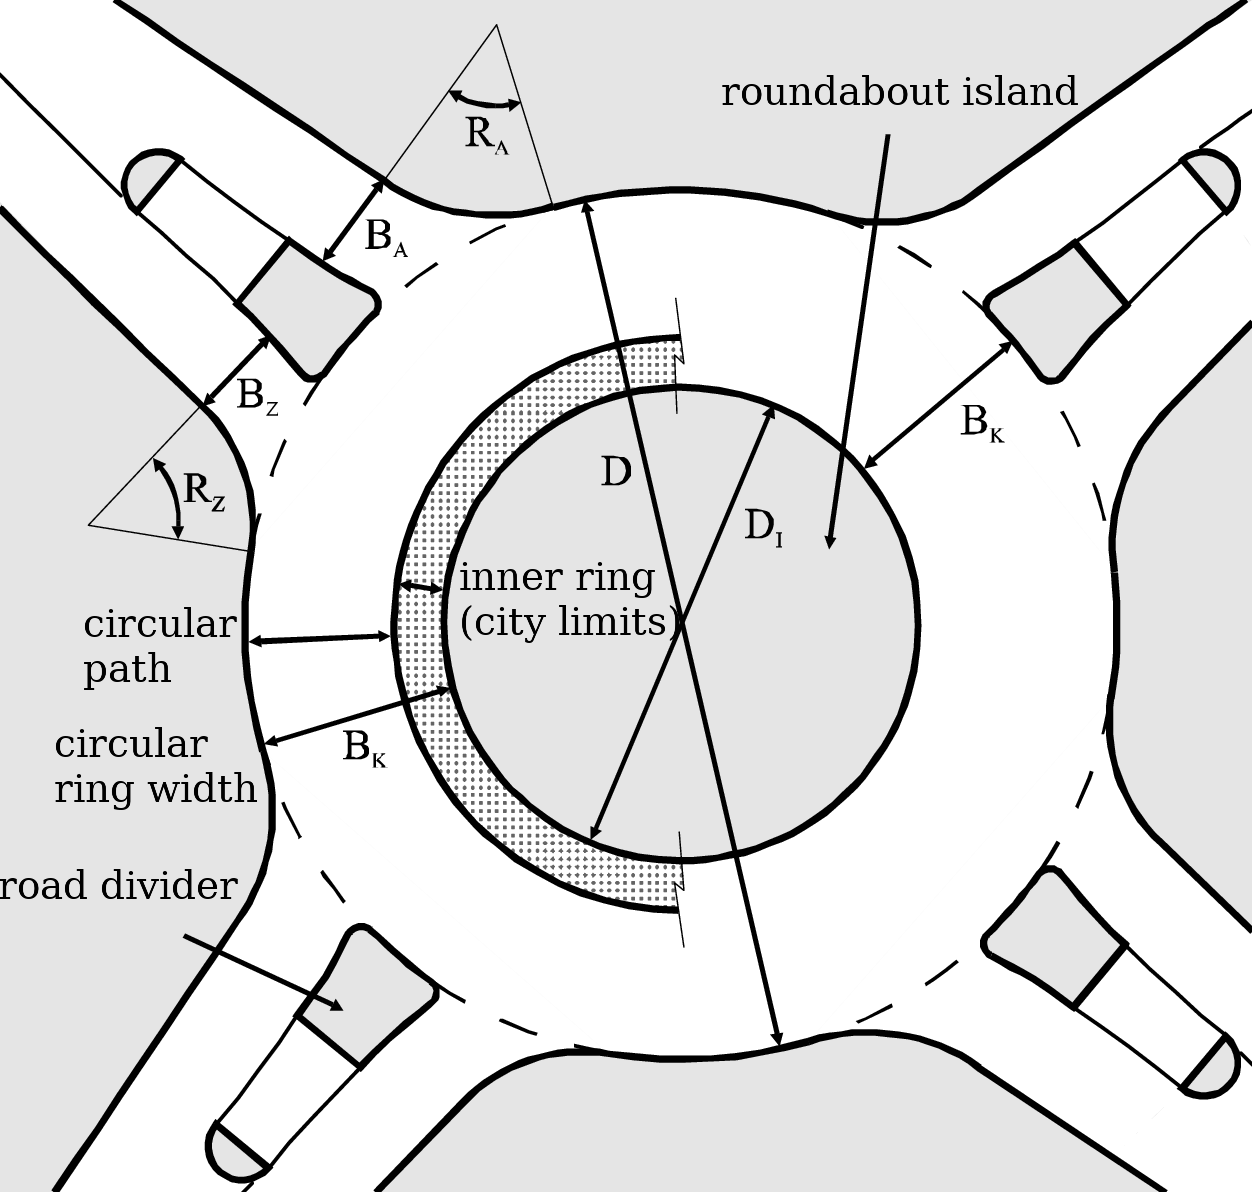
\includegraphics[width=0.7\textwidth]{bilder/kreisverkehr.png} %70% der Textbreite
\label{roundabout_parts}
%%\end{center}
\end{figure}


\begin{defi}[roundabout island]
The roundabout island is the constructional area in the middle of the roundabout, which is surrounded by vehicles.
For miniature roundabouts, the roundabout island is crossable.
\end{defi}

\begin{defi}[circular path]
%Die Kreisfahrbahn ist die Fahrbahn, die zum Umfahren der Kreisinsel
%dient. Ein ggf. vorhandener Innenring ist verkehrsrechtlich nicht Be-
%standteil der Kreisfahrbahn (VwV-StVO zu §9a V., Rn. 5).

%%TODO
The circular path is the road that serves to drive the roundabout island. An inner ring, if present, is not part of the circular path (VwV-StVO zu §9a V., Rn. 5).
\end{defi}

\begin{defi}[circular ring with ($B_K$)]
% Die bauliche Breite umfasst die Kreisfahrbahn und einen ggf. gepflasterten
% Innenring. Sie ist abhängig vom Außendurchmesser und der angestrebten
% Verkehrsführung (ein- oder zweistreifig). Die Randstreifenbreite orientiert
% sich an der maßgebenden durchgehenden Fahrbahn.
The structural width includes the circular track and a paved inner ring, if any. It is dependent on the outer diameter and the desired traffic routeing (one or two lanes). 
The edge strip width is oriented on the relevant continuous roadway.
\end{defi}

\begin{defi}[outer diameter ($D$)]
The outer diameter is measured at the outer edge of the circular ring. It is the essential measure for describing the size of the roundabout.
\end{defi}

\begin{defi}[inner diameter ($D_I$)]
The inner diameter is the diameter of the roundabout island.
\end{defi}

\begin{defi}[road divider]
% Der Fahrbahnteiler ist die baulich ausgeführte Insel zwischen Kreisausfahrt
% und -zufahrt einer angeschlossenen Straße. Er dient der Trennung der
% Kreisaus- und -zufahrten, der Führung des Verkehrs sowie den Fußgängern
% und Radfahrern als Überquerungshilfe.
%
The road divider is the structurally designed island between the circular exit
and circular driveway. It serves to separate the circular exit and circular driveway, the management of the traffic, as well as the pedestrians and cyclists as cross-bordering aid.
\end{defi}

\begin{defi}[lane width of the circular driveway ($B_Z$) and circular exit ($B_A$)]
% Die Breite der Kreiszufahrt und Ausfahrt wird am Beginn der Eckausrundung gemessen.
The width of the circular driveway and exit is measured at the beginning of the corner.
\end{defi}

\begin{defi}[Corner rounding radius ($R_Z$ and $R_A$) ]
% Dies ist der Radius der Ausrundung am rechten Fahrbahnrand zwischen 
% der Kreiszufahrt und der Kreisfahrbahn. Bei einem Korbbogen mit einer
% Radienfolge aus drei unterschiedlichen Radien ist RZ der Radius R2 des
% mittleren Bogens. Bei der Ausbildung des Fahrbahnrandes als Schleppkurve ist RZ der kleinste Radius des Fahrbahnrandes.
% 
This is the radius of the rounding at the right edge of the road between the circular driveway and the circular path.
For a elliptical arch with a radius sequence of three different radii, $R_Z$ is the radius $R_2$ of the central arc.
When the road edge is formed as a tractrix, $R_Z$ is the smallest radius of the road edge.
\end{defi}

\subsection{Types of Roundabouts}
There are several types of roundabouts, which are differentiated by the different application criteria and the partly different design principles according to the situation inside and outside built areas.
Furthermore, a division is made as a function of its size.


\subsubsection{Mini Roundabout}

\begin{figure}[!ht]
%\begin{center}
\caption{Mini Roundabout \cite{man06}}
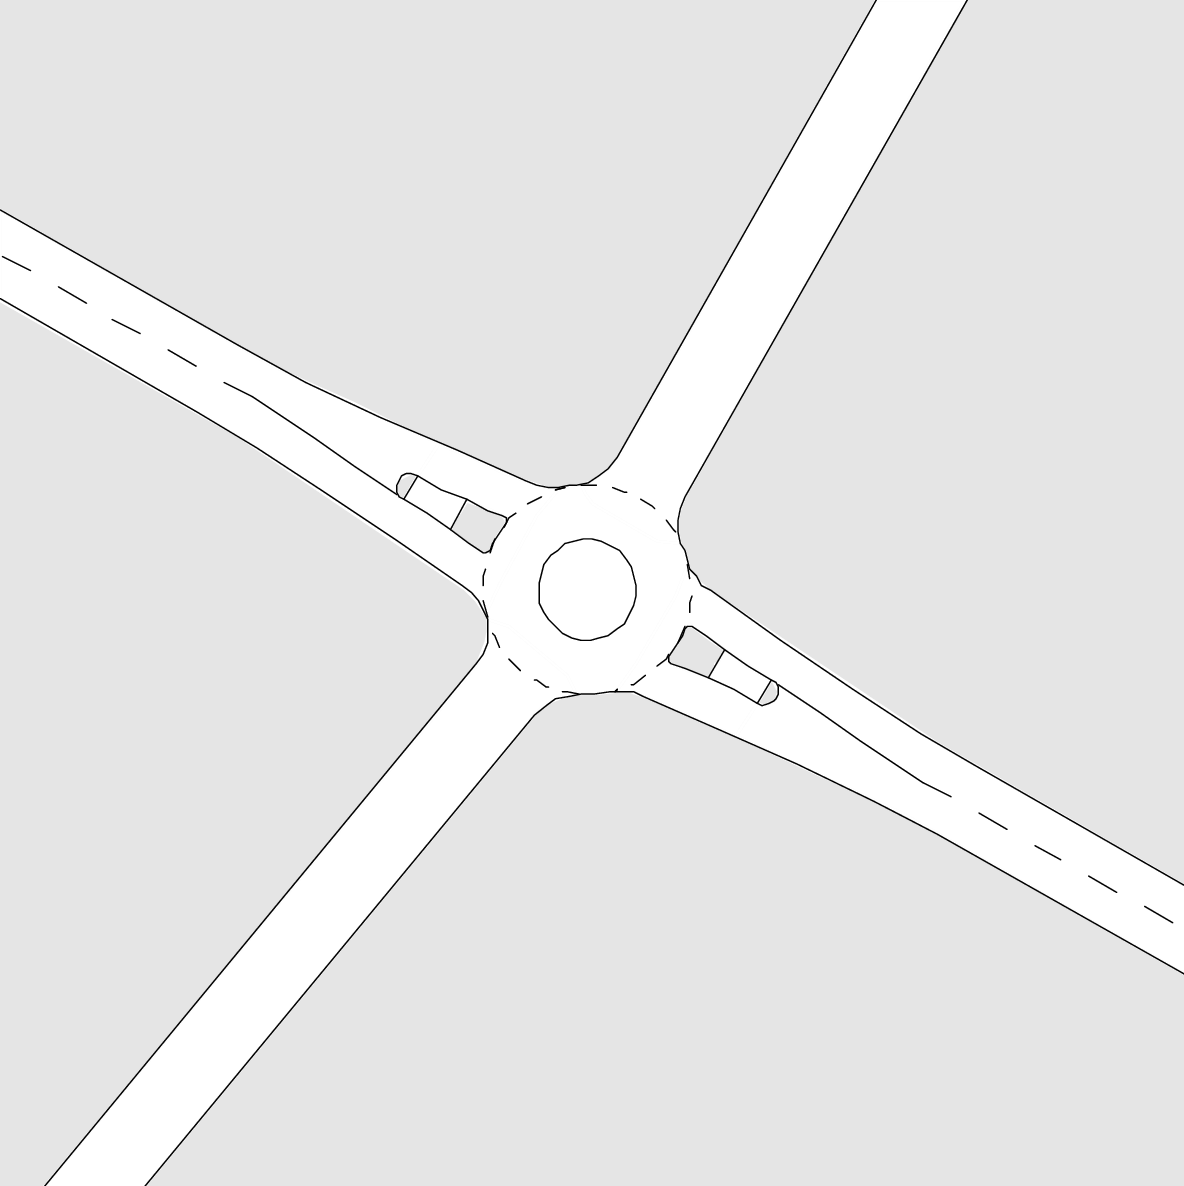
\includegraphics[width=0.5\textwidth]{bilder/mini_roundabout.png} %70% der Textbreite
\label{roundabout_mini}
%\end{center}
\end{figure}

Within built-up areas, smaller outer diameters are possible under certain conditions.
These roundabouts are called mini roundabout. The roundabout island must then be capable of being passed over.
The outer diameter should be at least 13 m, so that the circular island does not become too small.
Larger outer diameters make driving easier. Outer diameters of more than 22m, however, do not offer any transport advantages.
From an outside diameter of about 22 m, therefore, the installation of a small roundabout with 26 m is generally more convenient.
Bypasses are generally not required in the areas where mini roundabout can be used.


\subsubsection{Small Roundabout}

\begin{figure}[!ht]
%\begin{center}
\caption{Small Roundabout \cite{man06}}
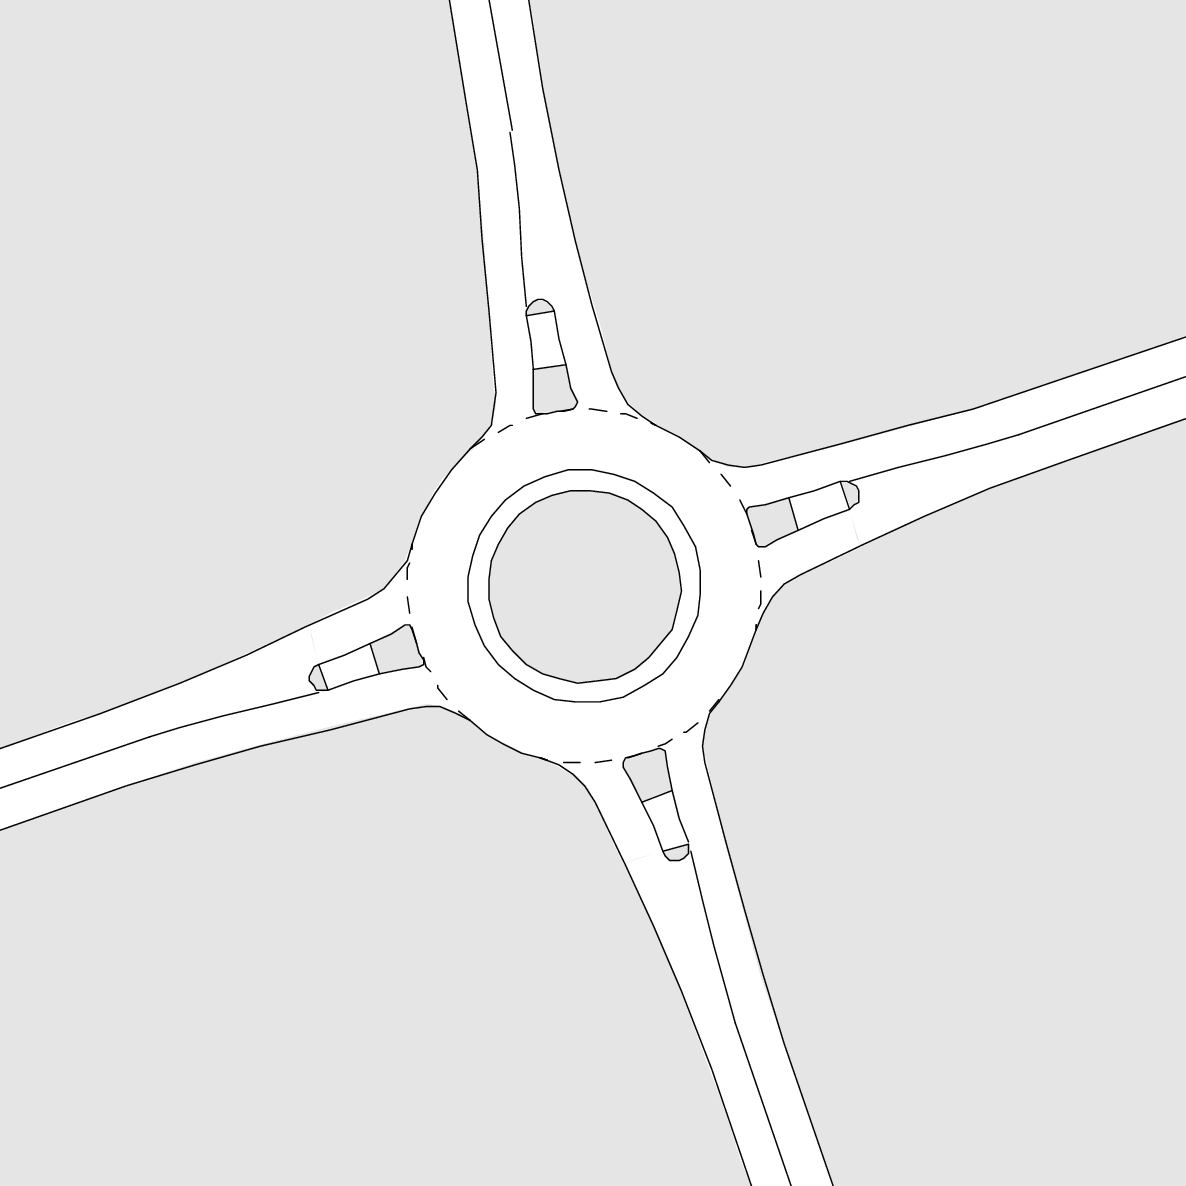
\includegraphics[width=0.5\textwidth]{bilder/small_roundabout.png} %70% der Textbreite
\label{roundabout_small}
%\end{center}
\end{figure}

The small roundabout has a single lane circular path and single lane circular driveways and exits. The roundabout island is not passable.
The outer diameter must be at least 26 m. Bypasses can be set up for driving geometric reasons or to increase performance.


\subsubsection{Two-lane Passable Roundabout}

\begin{figure}[!ht]
%\begin{center}
\caption{Two-lane Passable Roundabout \cite{man06}}
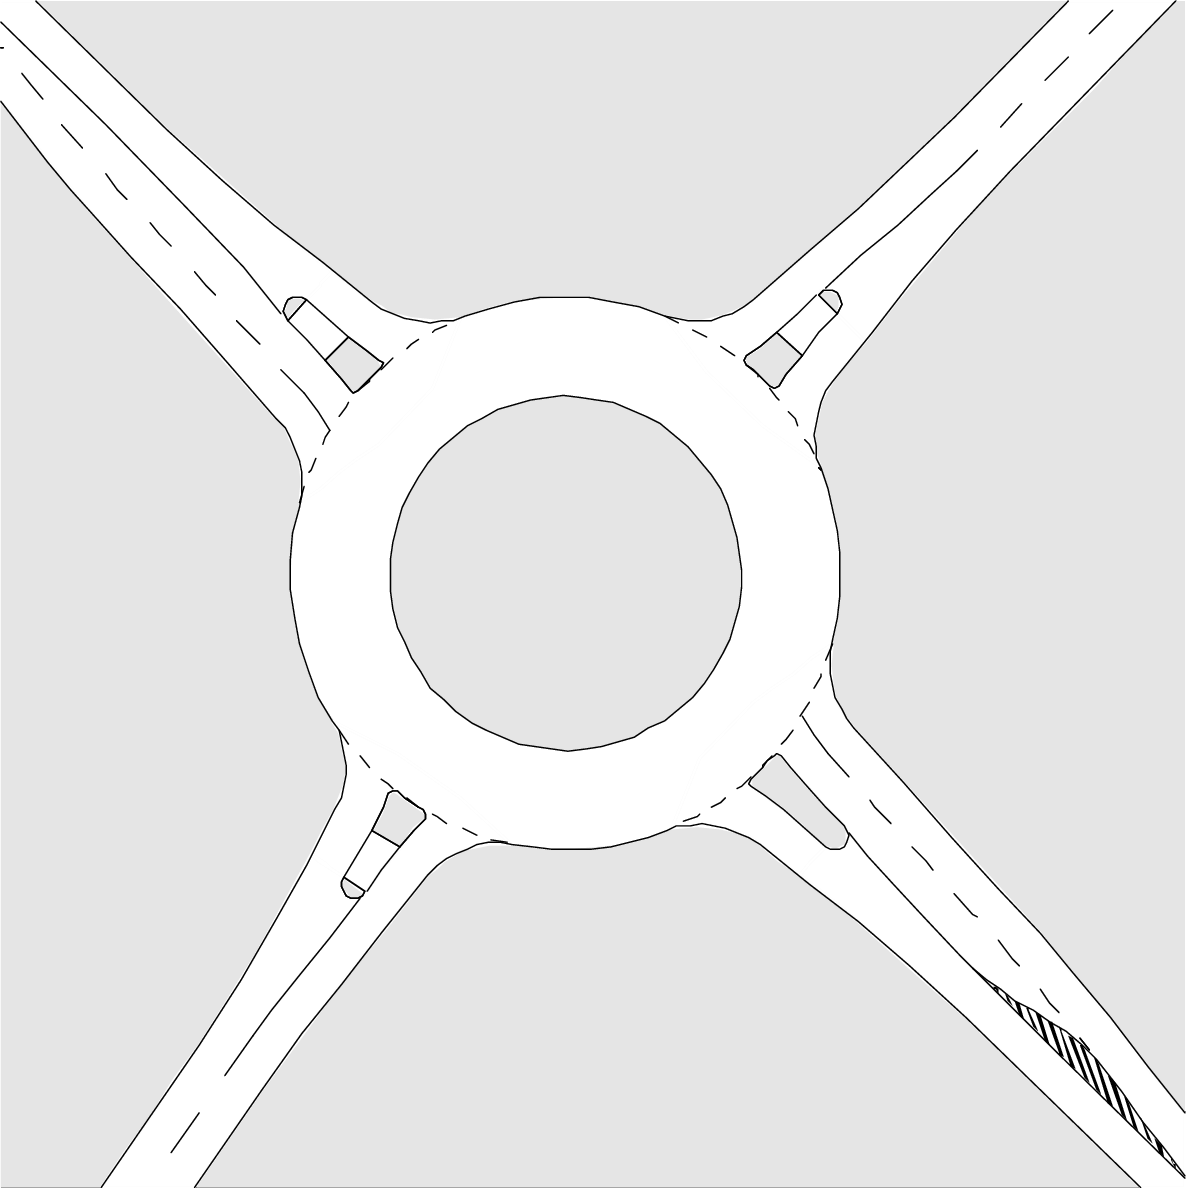
\includegraphics[width=0.5\textwidth]{bilder/twolaned_roundabout.png} %70% der Textbreite
\label{roundabout_twolaned}
%\end{center}
\end{figure}

% Reicht die Kapazität des Kleinen Kreisverkehrs nicht aus und kann diese nicht durch die Anlage von Bypässen sicher gestellt werden,
% kann die Kreisfahrbahn eines Kleinen Kreisverkehrs zweistreifig befahrbar ausgebildet werden.
% An einem solchen Kreisverkehr ist die Kreisfahrbahn so breit, dass Pkw im Kreis nebeneinander fahren können.
% Wird eine weitere Erhöhung der Kapazität erforderlich, können einzelne Kreiszufahrten ebenfalls zweistreifig ausgeführt werden,
% wenn Fußgänger und Radfahrer regelmäßig nicht zu berücksichtigen sind. Kreisausfahrten werden aus Sicherheitsgründen immer einstreifig ausgeführt.
% Aus geometrischen Gründen muss der Außendurchmesser bei zweistreifiger Befahrbarkeit mindestens 40 m betragen.
%
If the capacity of the small roundabout is not sufficient and can not be ensured by the installation of bypasses,
the circular path of a small roundabout can be designed to be two-lane driveable.
At such a roundabout, the circular path is so wide that cars can travel side by side in a circle.
If a further increase in the capacity is required, individual circular driveway can also be carried out in two lanes, if pedestrians and cyclists are not to be considered regularly.
For safety reasons, circular exits are always carried out in single lanes.
For geometrical reasons, the outer diameter must be at least 40 m for two-laned accessibility.


\subsubsection{Large Roundabout}


\begin{figure}[!ht]
%\begin{center}
\caption{Large Roundabout \cite{man06}}
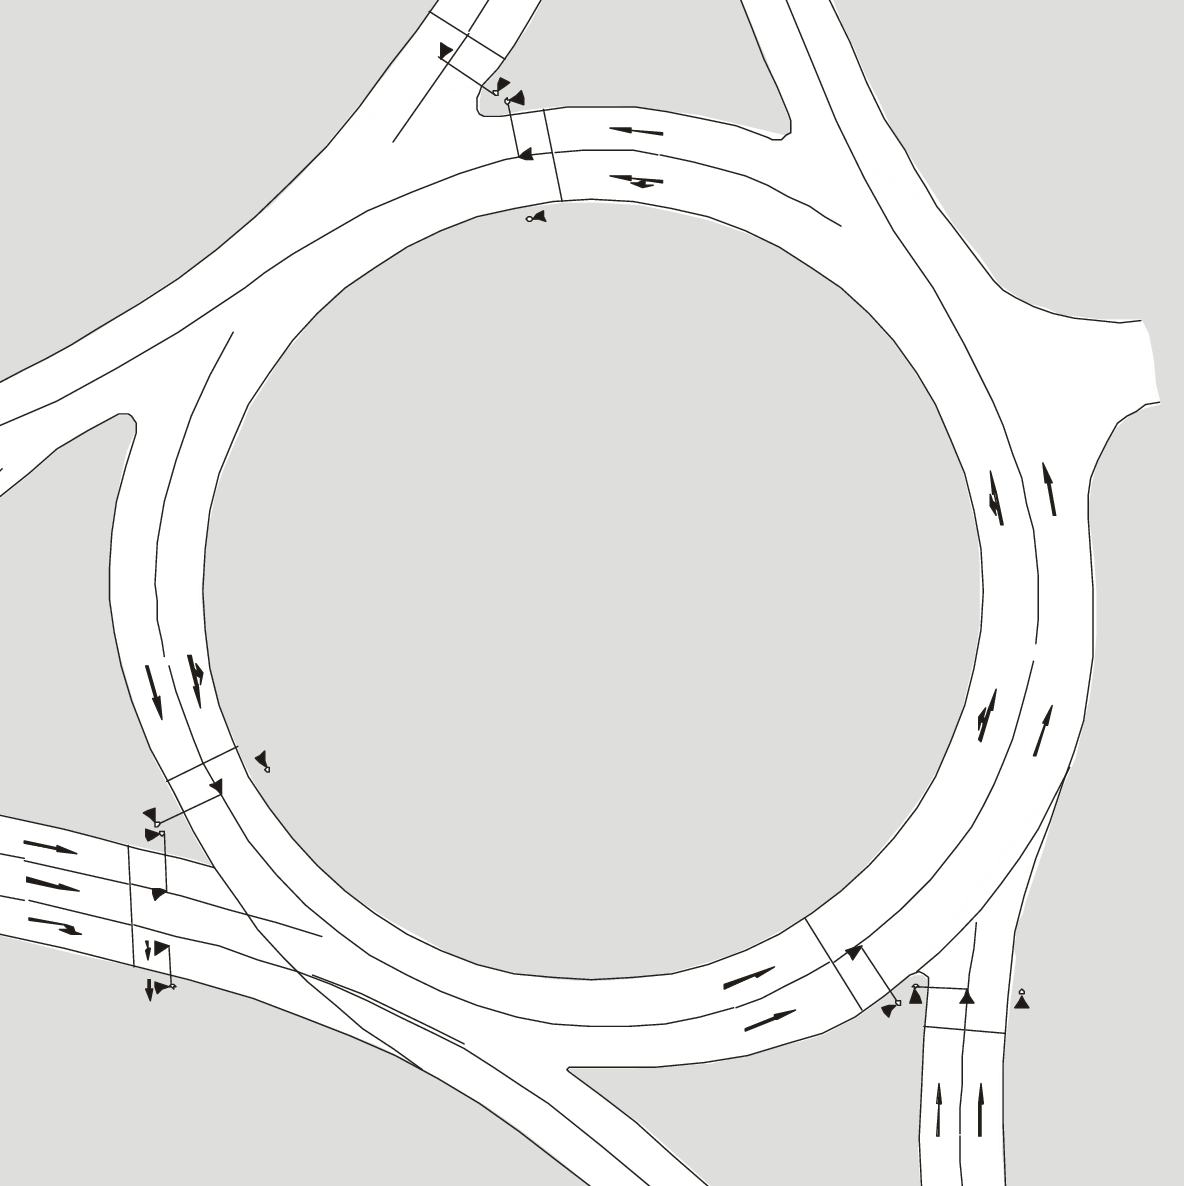
\includegraphics[width=0.5\textwidth]{bilder/large_roundabout.png} %70% der Textbreite
\label{roundabout_large}
%\end{center}
\end{figure}

%Große Kreisverkehre mit zwei oder mehreren durch Markierungen gekennzeichnete Fahrstreifen auf der Kreisfahrbahn sollen bei enger
%Abstimmung zwischen Knotenpunktentwurf und Verkehrssteuerung nur mit Lichtsignalanlage betrieben wer den.
Large Roundabouts with two or more lanes marked by markers on the circular path should be operated with a light signaling system only,
if the nodal point design and traffic control are closely coordinated.

\chapter{State of the Art}
% Auch wenn Autonomes Fahren ein aaktuelles Forschungsthema ist, gibt es bisher keine dem author bekannten veröffentlichungen welche sich explizit mit Kreisverkehren beschäftigen.
% Um trotzdem einen Verleich zur Sensoraustattung und Verkehrsbeobachtung zu haben werden an dieser Stelle einige Paper der \acs{DARPA} Urban Challenge herangezogen.
% Die DARPA Urban Challenge ist ein Rennen zwischen autonomen Fahrzeugen, welches im Jahre 2007 von der \ac{DARPA} ausgetragen wurde. \cite{Buehler2010} Das Rennen fand in bebautem Gebiet
% einer verlassenen Kaserne des ehemaligen Air Force-Stützpunktes George Air Force Base statt, die Karte kann ist in \cref{darpa_map} zu sehen.
Even if Autonomous Driving is an actual research subject, there are so far no publications known to the author, which deal explicitly with roundabouts.
In order to have a comparison to the sensor equipment and traffic monitoring, some papers of the \acs{DARPA} Urban Challenge are used here. 
The DARPA Urban Challenge is a race between autonomous vehicles, which was launched in 2007 by the \ac{DARPA} \cite {Buehler2010}.
The race took place in the built-up area of an abandoned barracks of the former Air Force base George Air Force Base, the map can be seen in \cref{darpa_map}
\footnote{\url{http://rsta.royalsocietypublishing.org/content/368/1928/4649}}.

\begin{figure}[!ht]
%\begin{center}
\caption{ \acs{DARPA} Urban Challenge Map }
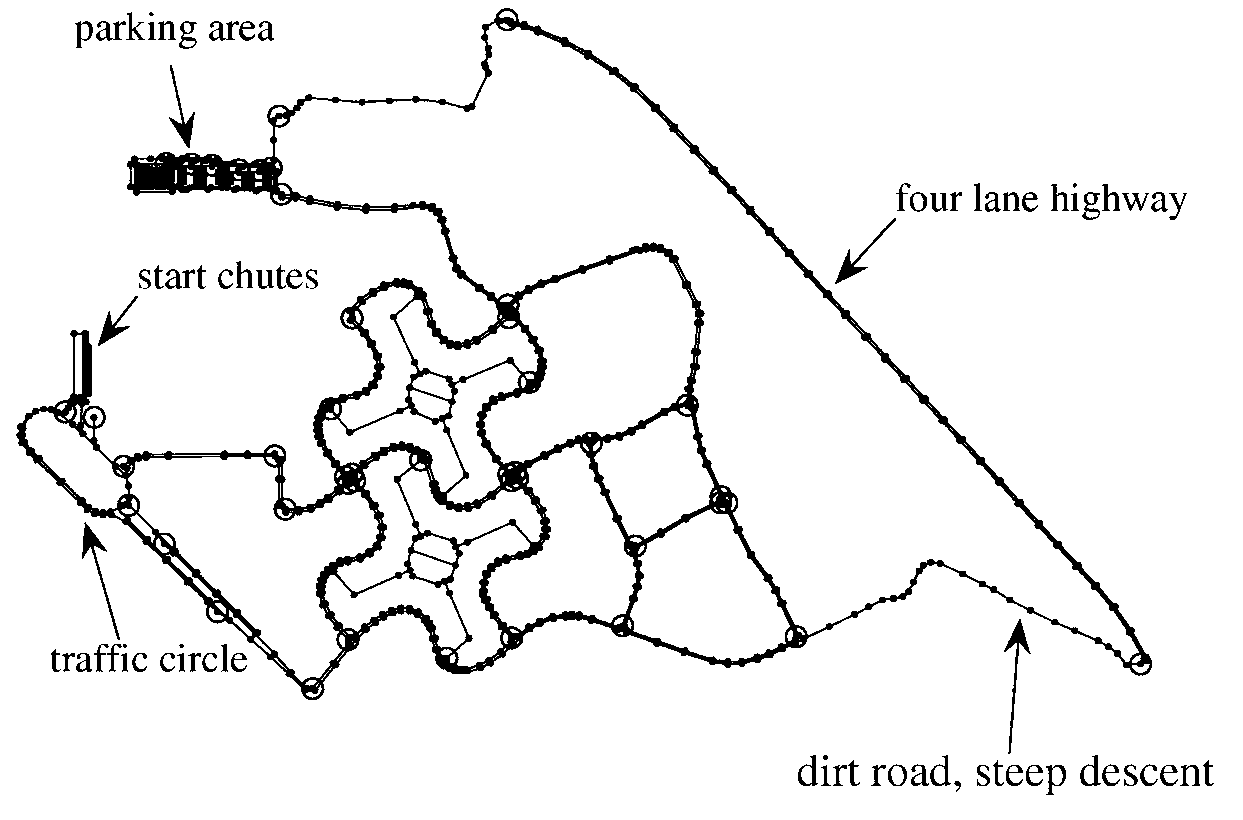
\includegraphics[width=\textwidth]{bilder/darpa_map_bw.png}
\label{darpa_map}
%\end{center}
\end{figure}

% Die Fahrbahnen waren teilweise durch Linien markiert, teilweise durch Betonwände begrenzt. Alle selbstfahrenden Autos befanden sich gleichzeitig auf der Strecke. 
% Auf ein-, zwei- und vierspurigen Straßen mussten Kreisverkehr, 4-Wege-Kreuzungen mit Stoppschildern, blockierte Fahrbahnen und Einfädelsituationen erfolgreich bewältigt werden.
The lanes were partially marked by lines, partially limited by concrete walls. All self driving cars were on the line at the same time.
On one-, two- and four-lane streets, roundabouts, 4-way intersections with stop signs, blocked lanes and threading situations had to be successfully managed.
 
% Bei der Auswertung  möchte ich mich vorallem auf die Finalteams des Wettbewerbes beschränken, da diese am Warscheinlichsten ein funktionierendes
% Konzept entwickelt haben. Ausgewertet werden dabei welcher Typ Sensoren und welche Anzahl die Teams für die Objekterkennung verwendet haben und 
% insoweit angegeben, welche algorythmen für Segmentierung und Tracking genutzt werden.

The evaluation is mainly limited to the final teams of the competition, since they have most likely developed a functioning concept.
The type and number of the sensors, for the object detection, used by the teams and the algorythms used for segmentation and tracking, if indicated, are evaluated.

% \begin{tabularx}{\textwidth}{|X|X|X|X|X|X|}
% \hline \textbf{Team} & \textbf{2D LiDAR} & \textbf{3D LiDAR (low res)} & \textbf{3D LiDAR (high res)} & \textbf{Radar} & \textbf{Camera}\\\hline
% Cornell \cite{Campbell2007} & 6 & 0 & 0 & 3 & 4 \\\hline
% TerraMax \cite{Corp2005} & 3 & 1 (4) & 0 & 0 & 3  \\\hline
% Stanford Racing Team \cite{Montemerlo2009} & 7 & 0 & 1 (64) & 3 & 1 \\\hline
% Tartan Racing \cite{Urmson2007} & 3 & 0 & 1 (64) & 2 & 1  \\\hline
% Victor Tango \cite{Atreya2007} & 1 & 1 (4) & 0 & 2 & 1  \\\hline
% \end{tabularx}

\section{DARPA Urban Teams}

\subsubsection{Team VictorTango}
% Team VictorTango \cite{Atreya2007} nutzt 2x Ibeo Alasca XT Sensoren, mit einer Reichweite von 200m und einem Öffnungswinkel von 240 Grad, um den vorderen Bereich des Fahrzeuges abzudecken, die beiden Sensoren werden komplementär fusioniert, um die vertikale Auflösung zu erhöhen.
% Jeder Sensor verfügt dabei über eine Vertikale Auflösung von 4 Lagen. Für den hinteren Bereich wird ein einzelnes 2D IBEO A0 LiDAR genutzt. Außerdem werden 4 Sick LMS291 LiDAR eingesetzt, 
% diese dienen jedoch nicht der Objekterkennung sondern werden Vertikal verbaut um die Fahrbahn in hoher auflösung nach Kanten abzusuchen. Die Onjektsegmentierung
% wird von Team VictorTango jedoch nicht selbst umgesetzt stadtdessen wird eine Komerzielle von Ibeo gelieferte ECU genutzt, welche die Daten der Ibeo Sensoren zu
% Objekten zusamenfasst. Die bereits fertig Segmentierten Objekte werden dann anhand der Road Detection gefiltert und anschließend von einer Softwarekomponente (Classification Center) zusammengefürt.
% Und innerhalb dieser gegen die Bildverarbeitung mit zwei 2D Kameras gegengeprüft. Eine Klassifizierung wird nur nach bewegten und unbewegten Objekten vorgnommen, als angnommen,
% das alle bewegten Objekte Autos sind. Das Team erreichte im Wettbewerb den dritten Platz \cite{Release2007}.

Team VictorTango \cite{Atreya2007} uses two Ibeo Alasca XT sensors, with a range of 200m and an opening angle of 240 degrees to cover the front area of ​​the vehicle, 
the two sensors are complementary fused to increase the vertical resolution. Each sensor has a vertical resolution of four layers. For the rear area, a single 2D Ibeo A0 LiDAR is used. 
In addition, four Sick LMS291 LiDARs are used, but these are not used for object detection but are installed vertically in order to search for edges on the road in high resolution.
However, the object segmentation is not implemented by Team VictorTango itself. In the meantime, a comercial ECU supplied by Ibeo is used, which directly detects objects in the data from the Ibeo sensors.
The objects already finished are then filtered using the Road Detection and are then combined by a software component (Classification Center). And within that counter-checked against image processing
with two 2D cameras. A classification is carried out only between moving and non moving objects, ie, all moving objects are cars. The team reached the third place in the competition \cite{Release2007}.
\subsubsection{Stanford Racing Team}

% Das Stanford Racing Team \cite{Montemerlo2009} ferfügt über eine Große Zahl von Sensoren unteranderm den großen Velodyne HDL-64E 3D LiDAR mit einer Vertikalen Auflösung von 64 Lagen, einer 360 Grad Rundumsicht und 120m reichweite.
% Dieser wird zusätzlich unterstützt von zwei SICK LD-LRS 2D LiDARs mit 250m reichweite am hinteren teil des Fahrzeuges, 2x Ibeo Alasca XT Sensore im vorderen Bereich sowie zusätzlich fünf Bosch
% Long Range Radare an der Front des Fahrzeuges. Zur Auswertung der Messdaten werden alle LiDAR Sensoren in einen  virtuellen 2D Laserscan transformiert. Dabei beschreibt das Team beim Velodyne Sensor
% Probleme mit Roll und Pitch Winkeln des Fahrzeuges welches zu False positives bei der Segentierung führen. Diese wurden dadurch korrigert, das die Messungen des Velodyne
% einen runden Kreis bilden (siehe\cref{stanford_junior_velodyne}). Diese Kreise haben bei korrekter Ausrichtung einen festen Abstand zueinander, über die betrachtung dieser Abstande konnte die Ausrichtung des Fahrzeuges korrigiert werden.
% Bei den 2D Sensoren wurde das Problem duch die Begrenzung der Reichweite behoben. 

The Stanford Racing Team \cite{Montemerlo2009} has a large number of sensors with the large Velodyne HDL-64E 3D LiDAR with a vertical resolution of 64 layers, 
a 360 degree panoramic view and a range of 120m. This is additionally supported by two SICK LD-LRS 2D LiDARs with 250m range at the rear of the vehicle, 2x Ibeo Alasca XT 
sensors in the front area and additional five Bosch long range radars at the front of the vehicle. To evaluate the measurement data, all LiDAR sensors are transformed 
into a virtual 2D laser scanner. The team describes, with the Velodyne sensor, problems with the roll and pitch angles of the vehicle which lead to false positives during the
segmentation. These were corrected by the measurements of the Velodyne forming a round circle (see \cref{stanford_junior_velodyne}). These circles have a fixed distance
from each other, if the alignment is correct. The roll and pitch angles of the vehicle can be corrected by looking at these distances. In the case of the 2D sensors, 
the problem was limited by limiting the range.

\begin{figure}[!ht]
\begin{center}
\caption{Velodyne HDL-64E Scan Rings \cite{Montemerlo2009}}
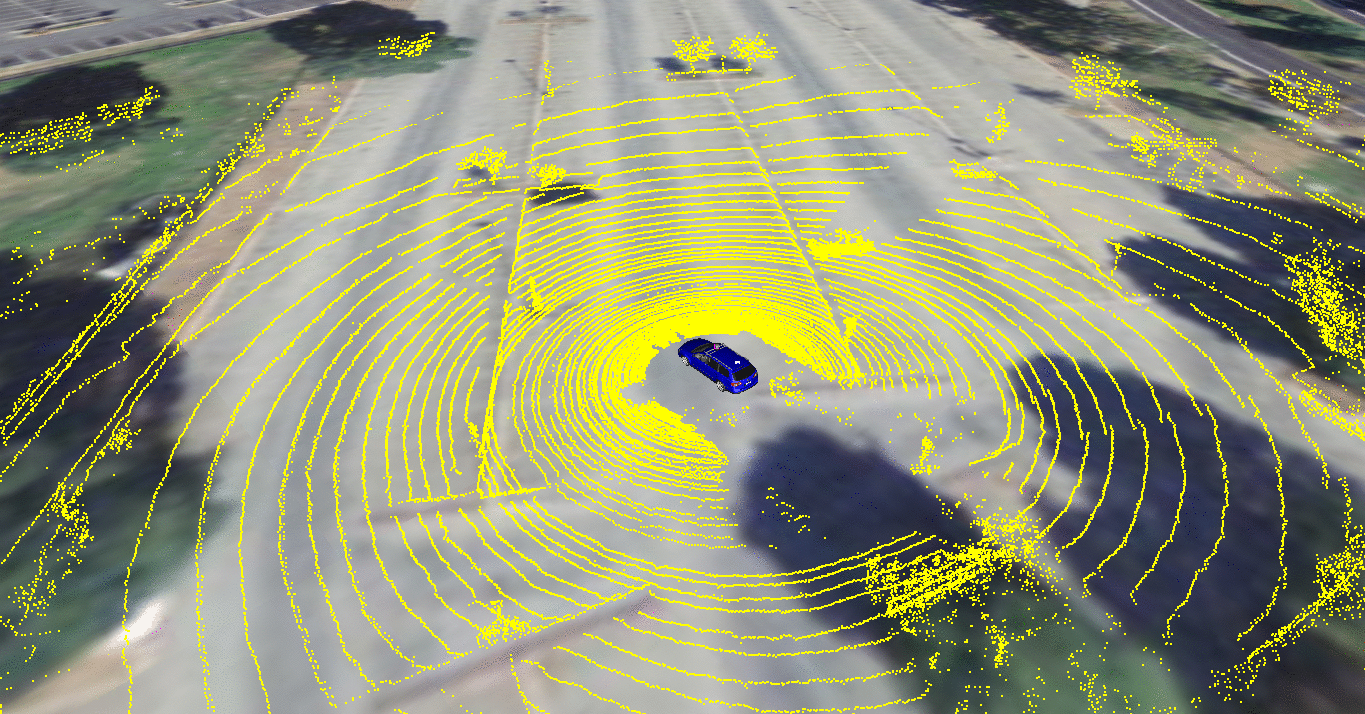
\includegraphics[width=0.7\textwidth]{bilder/stanford_junior_velodyne.png}
\label{stanford_junior_velodyne}
\end{center}
\end{figure}

% Zur Segmentierung der Objekte werden zwei Zeitschritte des Virtuellen Laserscans miteinaner verglichen. Bereiche in denen dabei eine Änderung detektiert wird werden dann als Onjekt klassifiziertund
% mithilfe eines Partikelfilters getrackt. Der Tracker schätzt dabei die Position, die Rotation, die Geschwindigkeit und die Größe des Objekts.
% Das Team erreichte im Wettbewerb den zweiten Platz  \cite{Release2007}.

For the segmentation of the objects, two time steps of the virtual laser scan are compared with one another. Areas in which a change is detected are then classified 
as objects and tracked using a particle filter. The tracker estimates the position, the rotation, the speed, and the size of the object.
The team reached the second prize in the competition \cite{Release2007}.


\subsubsection{Team Cornell}
% Team Cornell \cite{Campbell2007} nutzt für die Objekterkennung zwei seitliche Ibeo Alasca XT, ergänzend dazu werden drei RADAR Sensoren an der Fahrzeugfront genutzt welche es über den Doppler shift
% erlauben bewegte Objekte zu erkennen. Das Team hat auch einen Velodyne 3D LiDAR evaluiert sicha ber aufgrund des Preises und der Roll, Pitch Probleme für den Alasca XT entschieden,
% welcher 4 nahezu paralele Scans ausssendet und es so einfach macht, den boden zu erkennen. Über die Segmentierung der Objekte macht das Team keine Angaben, es wird lediglich gesagt, das die Sensorrohdaten
% in eine lokale Karte eingetragen, also fusioniert werden. Für das eigentliche Tracking wird ein ``Rao-Blackwellized Particle Filter''\cite{miller2007rao} genutzt.
Team Cornell \cite{Campbell2007} uses two side Ibeo Alasca XTs for the object detection. In addition, three RADAR sensors are used on the vehicle front, 
which allow the Doppler shift to detect moving objects. The team has also evaluated a Velodyne 3D LiDAR, but decided on the price and the roll, pitch problems
for the Alasca XT, which ejects 4 nearly parallel scans and makes it so easy to detect the ground. The team does not give any information about the
segmentation of the objects, it is merely said that the sensor raw data is written into a local map, ie fused. For the actual tracking a 
``Rao-Blackwellized Particle Filter'' \cite{miller2007rao} is used.

\subsubsection{TerraMax}
% Team TerraMax  \cite{Corp2005} nutzt ebenfalls den Ibeo Alasca XT und zusätzlich drei SICK LMS-291 LiDAR Sensoren Wobei der Ibeo Sensor frontal angebracht ist.
% Und die SICK Sensoren den seitlichen bzw hinteren Bereich abdecken. Weiterhin macht das Team intensiven gebrauch von einem selbt entwickelten Panorama Kamerasystem, das in idenischer ausführung
% einmal vorn und hinten moniert ist. Das System besteht jeweils aus 3 Kameras wobai abhängig von der geschindigkeit jeweils 2 Kameras genzuz werden um eine Stereobild der Umgebung zu berechnen.
% Bei höheren geschwindigkeiten wird auf die jeweiligen außeren Kameras umgeschalten, um eine höhere Tiefensicht zu erhalten. Um Objekte zu detektieren wird haupsächlich dieses System genutzt.
% Dabei wird von einer Flachen Fahrbahn ausgegangen, und alles was nicht flach ist als Objekt erkannt und dann mit den Rohdaten der LiDAR sensoren fusioniert.
% Team TerraMax beschreibt kein weiteres Tracken der Objekte.
Team TerraMax \cite{Corp2005} also uses the Ibeo Alasca XT and an additional three SICK LMS-291 LiDAR sensors. The Ibeo sensor is front-mounted and the SICK sensors 
cover the lateral or rear area. Furthermore, the team makes intensive use of a self-developed panorama camera system, which is mounted in an identical version, once
on the front and on the rear of the car. The system consists of three cameras each, depending on the speed, two cameras are used to calculate a stereo image of the environment.
At higher speeds, the respective outer cameras are switched over in order to obtain a higher depth of view. In order to detect objects, this system is mainly used.
In this case, a flat road is supposed, and everything which is not flat is detected as an object and then fused with the raw data of the LiDAR sensors. 
Team TerraMax does not describe any further tracking of the objects.

\subsubsection{Tartan Racing}
% Tartan Racing \cite{Urmson2007} nutzt eine kombination aus mehreren Sensoren zum Umfeldwarnehmung dabi ist der Velodyne HDL-64E, der Ibeo Alasca XT, ein ARS300 RADAR und diverse SICK 2D LiDARs.
% Die Segmentierung der Objekte wird dabei auf jedem Sensor einzeln durchgeführt und die Erkannten Objekte werden erst im darauf folgenden Schritt fusioniert. Über die Segmentierung macht
% das Team leider keine genauen angangen. Statische Objekte werden mithilfe einer cost map klassifiziert nund dynamische Objekte werden mit Hilfe eines Extendet Kalmanfiters und einem
% Constant Turn Rate and Acceleration (CTRA) Model getrackt und in eine Objektdatenbak eingetragen. Das Team erreichte im Wettbewerb den ersten Platz  \cite{Release2007}.
Tartan Racing \cite{Urmson2007} uses a combination of several sensors for environmental awareness, the Velodyne HDL-64E, the Ibeo Alasca XT, an ARS300 RADAR and various SICK 2D LiDARs.
The segmentation of the objects is performed individually on each sensor and the detected objects are fused only in the next step. Unfortunately,
the team does not make any precise statements about segmentation. Static objects are classified using a cost map and dynamic objects are tracked using an
Extended Kalman filter and a ``Constant Turn Rate and Acceleration'' (CTRA) model and written into an object database. The team reached the first place in the competition \cite{Release2007}.

\subsubsection{Team Caltech}
% Team Caltech \cite{Aly2007} nutz zur Objekterkennung vier Sick LMS 221, mit einer Reichweite von 30m aber einer hohen Frequenz von 75Hz, auf jeder seite des Fahrzeuges.
% Da das Team nur 2D Laserscaner verwendent, werden Objekte einfach Segementiert, indem Zusammenhängende Messungungen ohne Unterbrechung zusammengefasst werden.
% Danach werden die Werte in ein Lokales Koordinatensystem transformiert, Aufgrund der 75 Hz-Aktualisierungsrate der Sensoren und den relativ langsamen Geschwindigkeit der Fahrzeuge 
% im Rennen, kann eine gute verknüpfung von neuen Daten zu zuvor gesehenen Objekten einfach über ein Distanzkritterum gemacht werden. 
% Danach werden die Objekt an einen Kalman-Filter übergeben welcher Schätzposition und -geschwindigkeit aktualisiert,
% Wenn nach einer gewissen Anzahl von Beobachtungen die geschätzte Geschwindigkeit des Objekts über einer Schwelle liegt, wird es als Auto klassifiziert.
Team Caltech \cite{Aly2007} use four Sick LMS 221, with a range of 30m but a high frequency of 75Hz, on each side of the vehicle. 
Since the team only uses 2D laser scanners, objects are simply segmented by uniting neighbored measurements without interruption. 
After this, the values are transformed into a local coordinate system. Due to the 75 Hz update rate of the sensors and the relatively 
slow speed of the vehicles in the race, a good linkage of new data to previously viewed objects can easily be made over a distance criterion.
Then, the object is passed to a Kalman filter which is updated to estimate position and velocity. If, after a certain number of observations, 
the estimated velocity of the object is above a threshold, it is classified as a car.

\section{Conclusion}
% Wie wir gesehen haben, nutzen die teams teilweise sehr unterschiedlichs strategien um andere Fahrzeuge zu erkennen. Einige Teams führen die Segemntierung vor der Fusion der Daten durch,
% andere danach. Manche Teams nuzten eine Kombination aus Bildverarbeitung und LiDAR Sensoren, andere Vertrauen ausschließlich auf LiDAR Sensoren.
% Auffällig ist auch dass die beiden besten Teams (Tartan Racing, Stanford Racing Team) einen Velodyne HDL-64E nutzen, welcher im vergleich zu allen anderen Sensoren sie höchste auflösung 
% hat. Trotzdem wird dieser jedoch stets mit anderen Sensoren kombiniert, welche über eine höhere Reichweite verfügen. Vermutlich hatte die Sensorausstattung einen großen einfluss 
% auf den Ausgang des Wettbewerbes. Vergleicht man die Testfahzeuge der Teams mit unserem Testfahrzeug ``Snowfox'' ähnelt die Sensorausstattung am eheseten den Teams welch
% den Velodyne HDL-64E eingesetzt haben, welcher dem Velodyne VLP-16  ähnelt. Dieser von ``Snowfox'' genutzte VSensor war zum zeitpunkt des Wettbewerbes jedoch 
% noch nicht auf dem Markt \footnote{\url{http://www.spar3d.com/news/LiDAR/vol12no37-velodyne-announces-puck-LiDAR-sensor/}  [visited on 03/23/2017]}.
% Allerdings ist zu beachten, das der VLP-16 über eine signifikant niederigere Vertikae Auflösung verfügt als der HDL-64E, diese liegt jedoch immernoch
% über allen anderen verwendeten Sensoren. Allerdings muss ach gesagt werden, dass die Anforderungen in Wettbewerb unter denen dieses Projektes lagen.
% So war es im Wettbewerb nicht nötig zwischen verschienden Verkehrsteilnemern zu unterscheiden, da sich lediglich die Fahrzeuge der anderen Teams auf dem Parcour befanden.
% Da im Rahmen unseren Projekte auch andere Verkehrsteilnehmer wie Fußgänger und Radfahre erkannt werden müssen, stellt dies erhöte Anfordrungen an die Klassifisierung.
% Da Fußgänger und Radfahrer bedeutend kleiner sind als Fahrzeuge ist eine hohe Auflösung wünschenwert. 
% Ob der Sensor für seine Aufgabe geeignet ist, gilt es im folgenden zu untersuchen.

As we have seen, the teams share very different strategies to detect other vehicles. Some teams perform the segmentation before the fusing of the data, others afterwards.
Some teams used a combination of image processing and LiDAR sensors, others trusted solely on LiDAR sensors. 
It is also noticeable that the two best teams (Tartan Racing, Stanford Racing Team) use a Velodyne HDL-64E,
which has the highest resolution in comparison to all other sensors. Nevertheless, this is always combined with other sensors, which have a higher range. 
Presumably the sensor equipment had a great influence on the outcome of the competition. Comparing the test vehicles of the teams with our test vehicle ``Snowfox'' the sensor equipment
is most similar to the teams which have the Velodyne HDL-64E, which is similar to the Velodyne VLP-16.
However, this sensor used by ``Snowfox'' was not yet on the market at the time of the competition \footnote{\url{http://www.spar3d.com/news/LiDAR/vol12no37-velodyne-announces-puck-LiDAR-sensor/}
(03/23/2017)}. However, the VLP-16 has a significantly lower vertical resolution than the HDL-64E, but it is still above all other sensors.
However, it must be said that the requirements in competition were below those of this project. Thus it was not necessary in the competition to distinguish between 
different traffic, since only the vehicles of the other teams were on the course. As other traffic, such as pedestrians and cyclists, have to be detected as part of this project,
this places higher demands on classification and segmentation. Since pedestrians and cyclists are considerably smaller than vehicles, a high resolution is desirable. 
Whether the sensor is suitable for its task is to be investigated in the following.





\chapter{Methodology}
% Der eigentliche Kern der Arbeit. In diesen Kapiteln wird die Vorgehensweise methodisch
% erklärt. Oft werden fur Teilprobleme separate Kapitel angefertigt. Oft sind diese ¨
% Methodik-Kapitel aber auch logisch getrennt. Beispielsweise Kapitel fur ¨ Problemanalyse,
% Verfahrensauswahl, Umsetzung und Implementierung. Hinweis: Denken Sie daran:
% Diese Kapitel sind der Kern der Arbeit!! Sie sollten hier insbesondere klar herausstellen,
% was vorhandene Vorarbeiten sind und was im Rahmen dieser Arbeit entwickelt
% und umgesetzt wurde, also was Eigenanteil und was Fremdanteil ist

% Gefragt wird hier nach den Kriterien dafür, welche Methode für eine bestimmte Art der Anwendung geeignet ist,
% warum eine bestimmte Methode angewandt werden muss oder angewendet wird und keine andere.
% Verständnisfragen zum methodischen Weg werden hier geklärt.
% Die Methodologie ist demnach eine Metawissenschaft und somit eine Teildisziplin der Wissenschaftstheorie.
% Demgegenüber bezeichnet Methodik das Methodenwissen des Praktikers oder des Wissenschaftlers.

% Im vorigen Kapitel haben wir uns die Arten von Kreisverkehren und derren Komponenten angesehen.
% Weiterhin haben wir die zur verfügung stehende Testplatform und ihre Sensorik begutachtet. Dabei haben wir festgestellt, das für die Erkennung von Objekten in andren
% Arbeiten häufig mehrere und teurere Sensoren kombiniert werden um ein Zuverlässiges erkennen von anderen Verkehrsteilnehmern zu gewährleisten.

In the previous chapters we looked at the types of roundabouts and their components. We also reviewed the available test platform ``Snowfox'' and its sensor technology.
We have found that the detection of objects in other projects often combines several and more expensive sensors in order to ensure a reliable detection of other traffic users or
extend range.

% Wir der Zielsetzung haben wir festgehalten, das wir überprüfen wollen ob die Sensorausstattung des Testfahrzeuges ``Snowfox'' , 
% speziell der Velodyne VLP-16, für das Handling eines komplexen Verkehrszenarios, die Verkehrsbeobachtung eines Kreisverkehrs geeignet ist.

We have determined that we want to check whether the sensor equipment of the test vehicle `` Snowfox '', especially the Velodyne VLP-16, is suitable for the 
handling of a complex traffic scenario, the traffic monitoring of a roundabout.

% Dazu wird im folgenden ein Algorithms zum erkennen und Tracken von Objekten mit hilfe des Velodyne VLP-16 vorgeschlagen
% und implementiert. Die Schwierigkeit besteht dabei in der Verwendung eines Einzigen und im vergleich günstigen
% Umfeldsensors, welcher offensichtlich nicht als standalone Lösung für diesen Einsatzzweck entwickelt wurde.

For this purpose, an algorithm for detecting and tracking objects with the help of the Velodyne VLP-16 is proposed and implemented. 
The difficulty lies in the use of a single and in a comparatively low priced environmental sensor, which obviously has not been developed as a standalone solution for this purpose.

% Dieser Sensor bietet in seiner aktuellen Anwendung in dem für diese Arbeit relevanten Bereich eine vergleichsweise
% geringe Auflösung. Daher schlagen viele in ähnlichen Projekten genutzte Gradienten basierende Algorythmen im Bereich 
% der Segmentierung häufig fehl. \todo{beleg} Aus diesem Grund wird für die Segmentierung eine Groundplane basierender Algorithms implementiert.

In its current application, this sensor offers a comparatively low resolution in the area wich is relevant for this work.
Therefore, with many gradient-based algorythms, segmentation will often fail, beacuse the gradients becomes to smal.
For this reason, a ground plane based algorithm is implemented for the segmentation.

% Außerdem ist es Bauartbedingt in Kreisverkehren mit bebauten Mittelinseln und Mehrspurigen Kreisverkehren nötig
% Fahrzeuge über ihren Messhorizont hinaus zu verfolgen, um ein sicheres einfahren in den Kreisverkehr zu gerwährleisten.
% Zu diesem Zweck wird in Section \todo{section reference} ein Tracking und State Estimation Algorithms entwickelt welches dies gewähreisten soll.

In addition, it is necessary to follow vehicles beyond the measuring horizon in roundabouts, with built-up central islands and multi-lane roundabouts, 
in order to ensure a safe entry into the roundabout.
For this purpose, a tracking and state estimation algorithm is developed in \cref{tracking}, which should grant that.

% Zur Evaluation dieser Algorythmen wurden mehrere Datensammlungen auf den nahe gelegenen schwedischen AstaZero Prüfgelände in Sandhult [\cref{astazero}]
% durchgeführt, für alle nicht dort durchgeführten Expirimente werden in einer dafür erstellten Simulation durchgeführt. In dieser Simulation
% wird ein Innerstätischer Kreiverkehr mit Fuß un Radweg nachgebaut, welche der Kreisverkehr auf AstaZero nicht bieten kann.

In order to evaluate the sensor setup with these algorythms, were collected several data collections at the Swedish AstaZero test area nearby Sandhult (see \cref{astazero}
\footnote{\url{http://www.astazero.com/wp-content/uploads/2016/09/\%C3\%96versiktsskiss_mod.pdf} (03/24/2017)}).
Some other expiriments not carried out there, are carried out in a simulation made for this purpose. In this simulation a roundabout in a urban area 
with pavement and bikeway is designed, which the roundabout on AstaZero can not offer.

\begin{figure}[!ht]
%\begin{center}
\caption{AstaZero Proving Ground}
\includegraphics[width=\textwidth]{bilder/AstaZero.pdf}
\label{astazero}
%\end{center}
\end{figure}

% Die Evaluierung findet dabei von Hand anhand der grafisch aufbereiteten Messdaten statt. Dabei wird besonders auf False-Negativ
% und False Positiv erkannte Hindernisse eingegangen. Grobe Außreißer bei der Position oder Orientierung dr Objekte werden ebenfalls verkmerkt.

The evaluation is carried out manually by using of the graphically prepared measurement data. 
While the evaluation especially False-Negative and False-Positive detected obstacles will be discussed.
Coarse outliers in the position or orientation of objects are also noted. Also, a performance analysis is made.

% Zur Evaluation der Handbarkeit des Kreisverkehrs wird außerdem eine Statemachine Implementiert welche das Fahrzeug Sicher und Unfallfrei
% durch den Kreiverker bewegen soll. Dazu wird die Simulation über einen längeren Zeitraum beobachtet, und die Anzahl der eventuellen
% Kollisionen notiert.

In order to evaluate the operability of the roundabout, a state machine is implemented which is intended to move the vehicle safely and accident-free through the roundabout.
For this purpose, the simulation is monitored over a longer period of time and the number of possible collisions is noted.


\chapter{Sensor Analysis}
% Wie bereits diskutiert wird sich die auswahl der Senoren auf das Applanix POS-LV und den Velodyne VLP-16 beschränken. Da der Velodyne für die 
% erkennung anderer Verkehrsteilnehmer der wichtigste sensor ist, wird nun untersucht, in wie fern der Sensor für die Ekennung geeignet ist.

As already discussed, the selection of senors will be limited to the Applanix POS-LV and the Velodyne VLP-16. Since the Velodyne is the more
important sensor for the recognition of other traffic users, it is now investigated how far the sensor is suitable for the detection.

\section{Theoretical Analysis}
% Unter \cref{types_of_roundabouts} haben wir vier verschieden Typen von Kresiverkehren festehalten. Um die den Praktischen nutzetn des Velodyne VLP-16
% zu bewerten wird nun Analysiert, in wie fern dieser in der lage ist diese Zu überblicken. Dazu sehen wir uns im folgenden die Größenverhältnisse  an.

Under \cref{types_of_roundabouts} we have established four different types of roundabouts. In order to evaluate the practical use of the Velodyne VLP-16 is now analyzed,
how far the Velodyne is able to overlook the situation. For this purpose we will look at the size ratios.


\begin{tabularx}{\textwidth}{|X|X|X|}
\hline \textbf{Roundabout Type} & \textbf{min Size} & \textbf{max Size} \\\hline
Mini Roundabout& 13m & 22m \\\hline
Small Roundabout& 26m  & 40m \\\hline
Two-lane Passable Roundabout& 40m & - \\\hline
Large Roundabout& >40m &  - \\\hline
\end{tabularx}

% Um nun ein Vergleich zum Velodyne VLP-16 zeihen zu können, sehen wir uns den sichtbereich des Sensors von der seite an.
% Der Sensor liefert uns 16 Messungen im selben Azimuthwinkel, im Abstand von 2 Grad. Da für die Ausertung, und leider auch für die Erkennung, die Winkel größer als 0 Grad 
% nicht relevant sind sehen wir uns nur die acht winkel im bereich von -1 bis -15 Grad an. 

For a comparison to the Velodyne VLP-16, we will look at the visual range of the sensor in the 2D side view. The sensor provides 16 measurements at the same azimuth angle,
with a distance of 2 degrees.Since for the evaluation, and unfortunately also for the detection, the angles greater than 0 degrees are not relevant, because they look into
the air. So we only see the eight angles in the range of -1 to -15 degrees.

% Bei der auswertung gehen wir davon aus, das wir versuchen einen Kleinwagen mit einer länge von 4 Metern und 1.5 Metern höhe zu erkennen. Dabei gehen wir von dem Idealfall aus, das sich das Fahrzeug
% auf uns zu bewegt. Weiterhin gehen wir von einer Befestigungshöhe des Sensors von 2.1 Metern aus, da dies letztendlich die montagehöhte des Sensors uf dem Testfahrzeug darstellt.

In this evaluation we assume that we try to detect a small car with a length of 4 meters and 1.5 meters height. In doing so, we start from
the ideal situation that the vehicle drives in your direction.
Furthermore, we assume a mounting height of the sensor of 2.1 meters as this is finally the mounting height of the sensor on the test vehicle.

\paragraph{Range 0-25m}
% Für den Bereich von 0m bis 25m sehen wir in \cref{velodyne_range_25}, dass wir im schlimmsten fall noch eine Messung vom Sensor erhalten. Befindet sich das Fahrzeug sehr nache am 
% Sensor erhalten wir sogar einen Großteil der zur verfügung stehenden Auflösung, wobei dabei sich nahe dahnter befindliche flache Fahrzeuge verdeckt werden können. 
% Daher sehen wir, das der Mini Roundabout mit dem Sensr geut abgedeckt werden kann, wir uns jedoch gendanken über verdeckte hindernisse machen müssen.

For the range from 0m to 25m, we see in \cref{velodyne_range_25} that in the worst case, we still get at least one measurement from the sensor. 
Is the vehicle very much at the
Sensor, we get even a large part of the available resolution, whereby close to behind lying flat vehicles can be hidden. Therefore, we can see 
that the mini roundabout can be covered with the sensor, but we have to think about hidden obstacles.

\begin{figure}[!ht]
%\begin{center}
\caption{Velodyne VLP-16 - Range 0-25m}
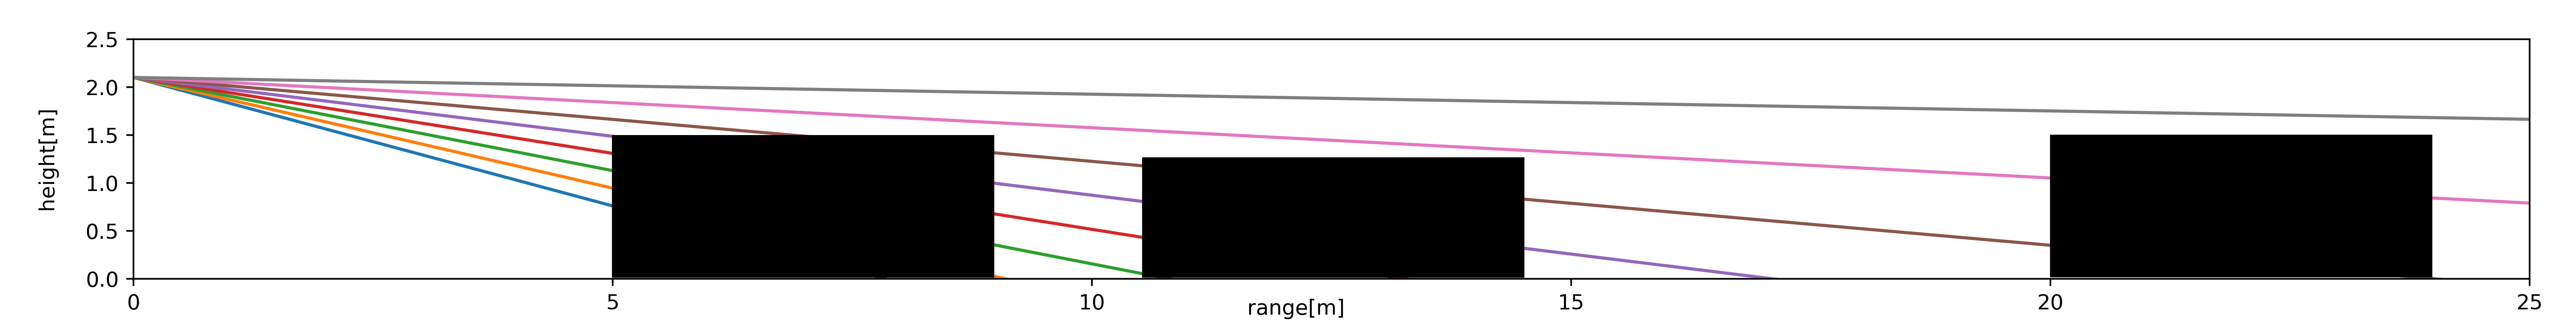
\includegraphics[width=\textwidth]{bilder/range_25.png}
\label{velodyne_range_25}
%\end{center}
\end{figure}

\paragraph{Range 25-50m}
% Für den Bereich von 25m bis 50m sehen wir in \cref{velodyne_range_50}, dass wir im grunde nur noch zwei Messungen erhalten können. Für unseren angenommenen Kleinwagen mit einer Höhe von 1.5 Metern
% ehalten wir jedoch keinen Totereich. Jedoch erhalten wir für die meißten messungen nur einen Messpunkt und somit eine sehr niedrige Auflösung. Daher ist die Erkennung von Fahrzeugen
% in einerm kleinen Kreisverkehr bereits eine herausforderung für die Segmentierung der Fahrzeuge

For the range of 25m to 50m we see in \cref{velodyne_range_50} that we can only get two measurements. For our assumed small car with a height of 1.5 meters,
however, we do not keep a dead zone. However, for most measurements, we get only one measurement point and thus a very low resolution.
Therefore the detection of vehicles in a small roundabout is already a challenge for the segmentation of the vehicles

\begin{figure}[!ht]
%\begin{center}
\caption{Velodyne VLP-16 - Range 25-50m}
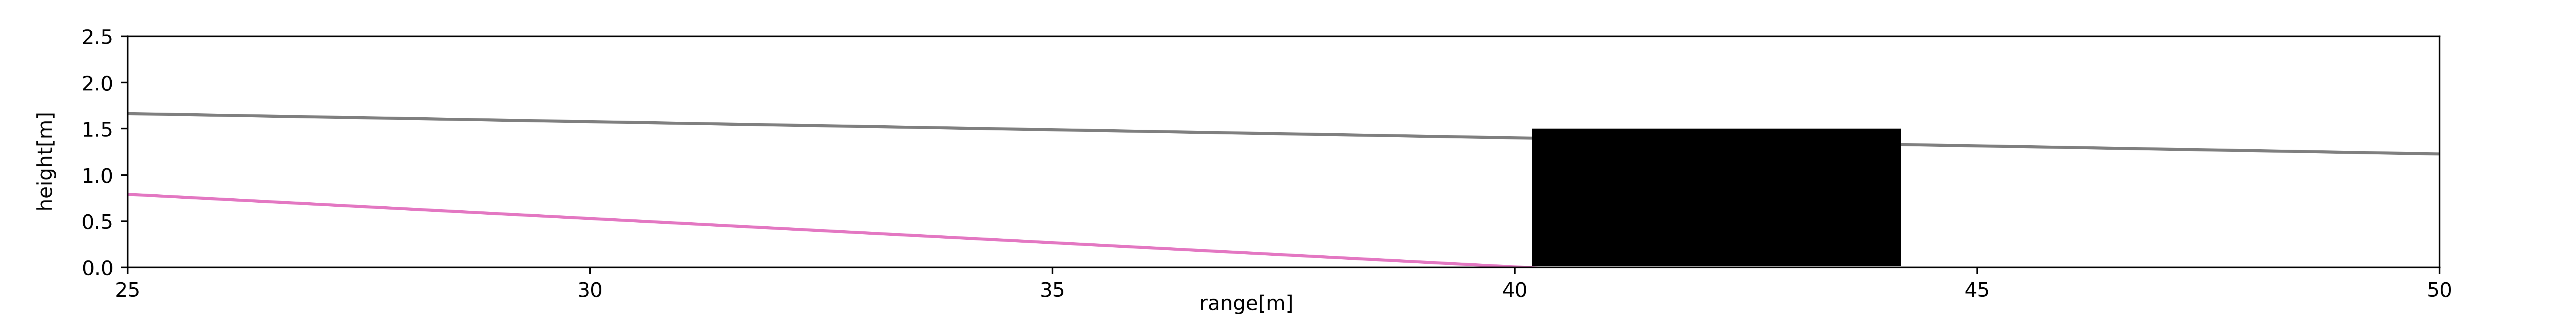
\includegraphics[width=\textwidth]{bilder/range_50.png}
\label{velodyne_range_50}
%\end{center}
\end{figure}

\paragraph{Range >50m}
% Für den Bereich größer als 50m sehen wir in \cref{velodyne_range_75}, dass die Auflösung im verleich zu näheren Objekten gleich bleibt. Jedoch steigt hier die Warscheinlichkeit, dass
% fahrzeuge bereits im voherigen bereich verdeckt wurden.

For the area greater than 50m, we see in \cref{velodyne_range_75} that the resolution remains the same in the same way as for closer objects.
However, there is a higher likelihood that vehicles have already been hidden in the previous area.

\begin{figure}[!ht]
%\begin{center}
\caption{Velodyne VLP-16 - Range 50-75m}
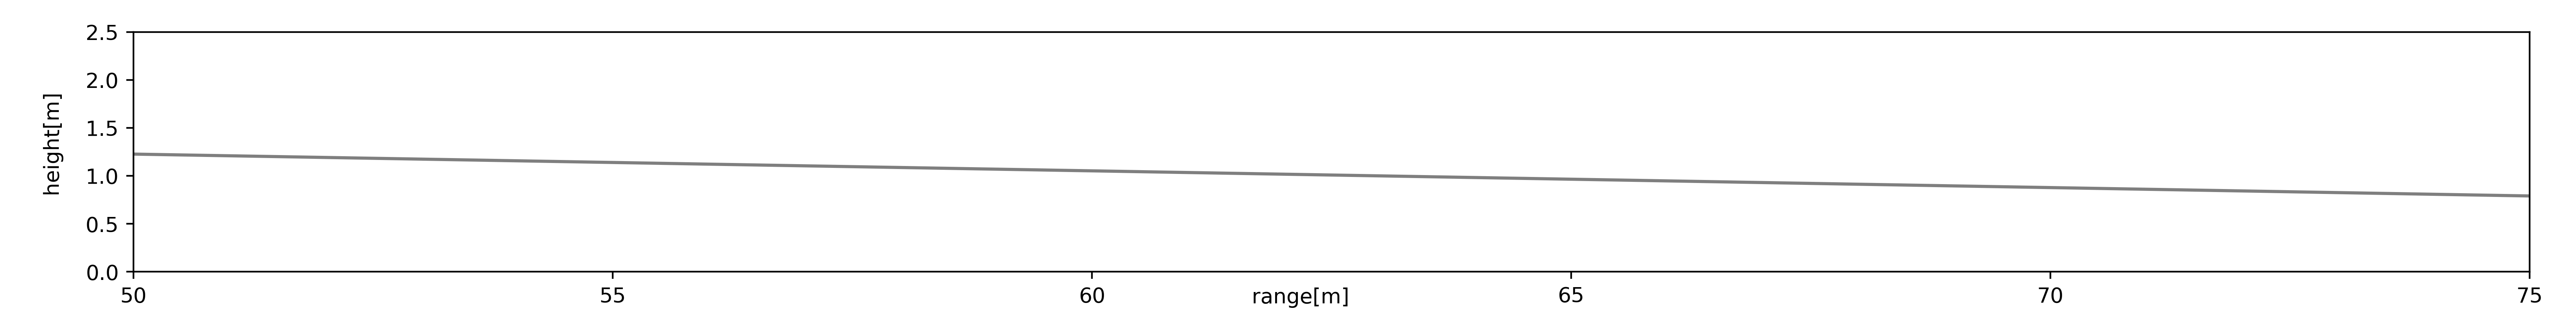
\includegraphics[width=\textwidth]{bilder/range_75.png}
\label{velodyne_range_75}
%\end{center}
\end{figure}



% Wie wir sehen  können wir den Bereich bis 25 Metern gut abdecken und somit den Mini Roundabout komplett beobachten, für Größere Kreisverkehre ist der Sensor nur bedingt geeigent.
% wesshalb wir für alle folgenden Betrachtungen nur Minikreisverkehre oder kleinere kleine Kreisverkehre betrachten werden. Für alle anderen Kreisverkehre, währe zu
% evaluieren, ob es überhaupt nötig ist, alle Fahrzeuge im Kreisverkehr zu beobachten, da die Strecke von Einfahrt zu Einfahrt entsprechend größer wird.
% Eventuell ist es so möglich den Kreisverkher als einfache Vorfahrtsituation zu betreachten.

As we can see, we can excellent cover the area up to 25 meters and thus observe the mini roundabout completely, for larger roundabouts the sensor is only conditionally suitable. 
For all the following considerations, we shall consider only miniature circuits or smaller small roundabouts. 
For all other roundabouts, evaluate whether it is necessary to observe all the vehicles in the roundabout, as the distance from driveway to driveway increases accordingly.
It is maybe possible to consider the roundabout as a simple yield sign situation.

\section{Practical Analysis}
% Da wir uns nun bereits die Theoretischen überlegungen angesehen haben sehen wir uns die praktischen Messungen des Sensors an. 
% Dazu können wir in \cref{velodyne_hidden} eine Messung auf dem Testkreisveker auf AstaZero in der Vogelperspektive sehen.

Since we have already looked at the theoretical considerations, we look at the practical measurements of the sensor.
To do this, we can see a measurement on the test roundabout on AstaZero in the bird's eye view in \cref{velodyne_hidden}.

\begin{figure}[!ht]
%\begin{center}
\caption{Velodyne VLP-16 - Hidden Layers}
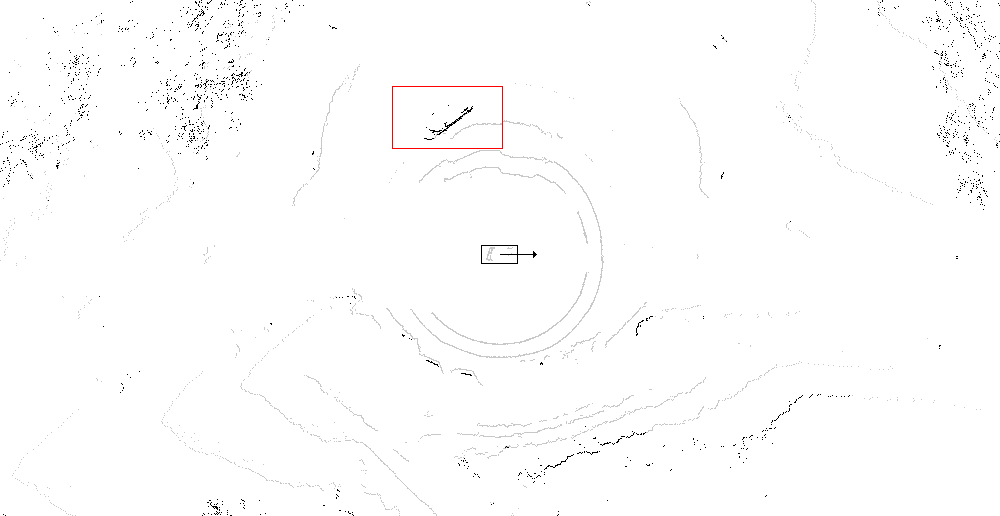
\includegraphics[width=\textwidth]{bilder/velodyne_back.png}
\label{velodyne_hidden}
%\end{center}
\end{figure}

% Dort ist zu erkennen, dass die Messungen im vorderne und vorallem im hinteren Bereich Lücken aufweisen. Dies ließ sich bei der Montage des Velodyne leider nicht verhindern,
% da die Haltevorrischtung des Sensors keine weitere Höhenverstellung vorsieht und am Testfahrzeug keine invasiven Änderungen vorgenommen werden sollten.
% Daher musste für die Montage ein kompromiss geschlossen werden, entweder messungen im vorderen Bereich zu verlieren ider im Hinteren. Die Fahlenden Messungen werden
% vom Fahrzeugdach verdeckt. Die Kleineren lücken im vorderen Bereich stammen von der GPS Antenne des Aplanix Systems und ließ sich leider auch nicht verhindern.

It can be seen here that the measurements in the front and especially in the rear region have gaps. Unfortunately, this can not prevented during installation of the Velodyne since 
the holding pre-treatment of the sensor does not provide a further height adjustment and no invasive changes should be made to the test vehicle. 
Therefore, a compromise had to be concluded for the assembly, either to lose measurements in the front area, or to lose in the rear.
The missing measurements are obscured by the vehicle roof. The smaller gaps in the front area come from the GPS antenna of the Applanix system and unfortunately also 
could not be prevented.

% Da die Beocbachtung des Hinteren Bereiches für die Kreisverkehrbeobachtung nicht wichtig ist sind die Fehlenden Messungen im Hinteren Bereich jedoch zu vernachlässsigen.
% Da wir im vorderen Nahebereich des Sensors die höchste Auflösung haben fallen die fehlenden Messungen im im Frontbereich auch nicht ins gewicht, denn diese befinden sich 
% nur im ersten Messlayer.

Since the monitoring of the rear area is not important for the roundabout observation, the missing measurements in the rear area are negligible. 
Since we have the highest resolution in the front area of the sensor, the missing measurements in the front range are not important,
also these are only in the first measurement layer.


% Weiterhin in \cref{velodyne_hidden} zu sehen ist es weiteres Testfahrzeug (rote box). An diesem ist zu erkennen, das wir auch im eigentlich verdeckten hinteren Bereich des Fahrzeuges
% Messungen erhalten. Dies ist dadurch zu erklären, dass der Sensor über mehrere Return Modes verfügt, die es Ihm erlaubt durch Transparente Objekte zu sehen. Dies kann in \cref{vel_trans}
% gesehen werden

Further in \cref{velodyne_hidden} to see is another test vehicle (red box). It can be seen from this that we also get measurements in the rear of the vehicle, which is actually hidden.
This is explained by the fact that the sensor has several return modes, which allows it to see through transparent objects. This can be seen in the example in \cref{vel_trans}.

\begin{figure}[!ht]
%\begin{center}
\caption{Velodyne VLP-16 - Return Modes \cite{manVEL}}
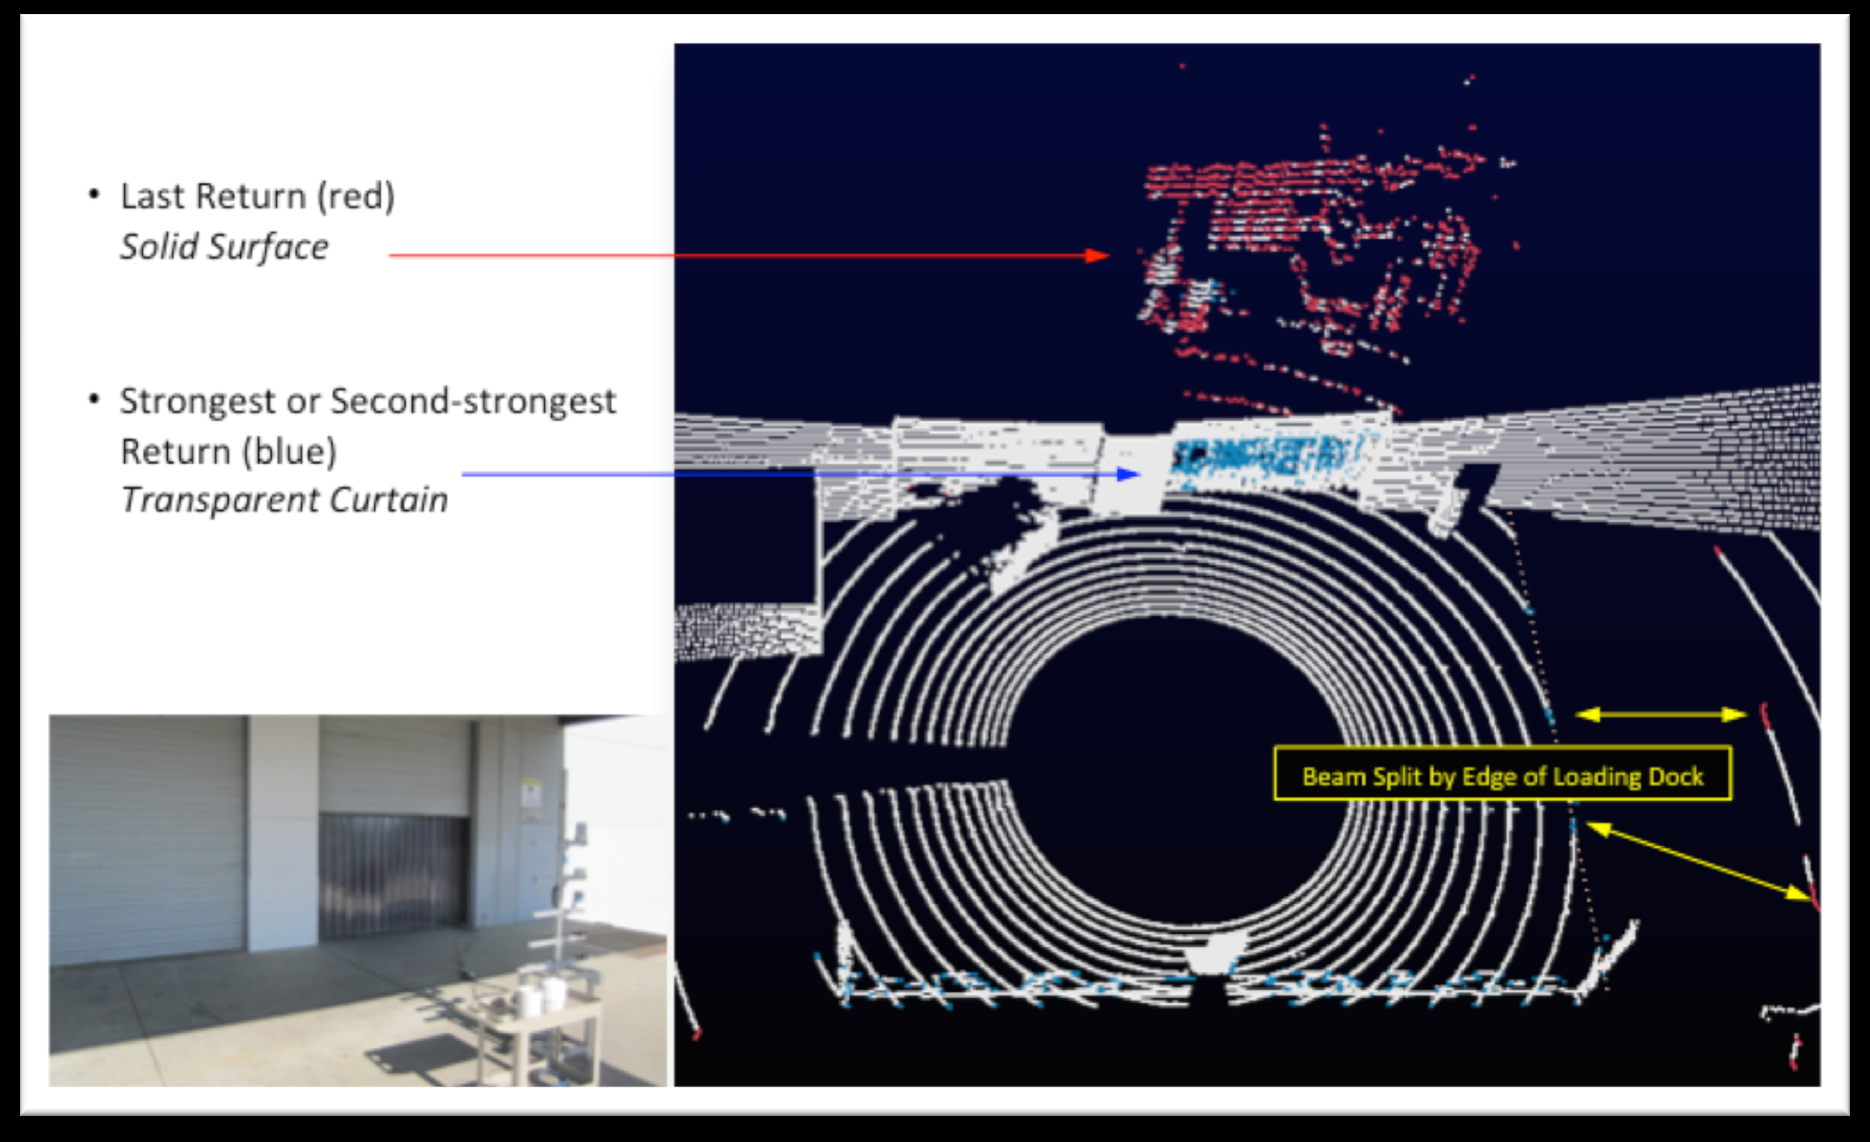
\includegraphics[width=\textwidth]{bilder/velodyne_trans.png}
\label{vel_trans}
%\end{center}
\end{figure}

% Der Sensor kann dabei so konfiguriert werde, dass er beide Messungen (Strongest Return und Last Return) zurückliefert. Da die zu beobachten Fahrzeuge nicht vollständig transparent
% sind und so immer auch ausreichend messungen im vorderen Bereich liefern , ferner um die Datenrate klein zu halten wurde dir VLP-16 so konfiguriert, dass
% er nur den Last Return liefert.

The sensor can be configured to return both measurements (Strongest Return and Last Return). Since the vehicles to be observed are not completely transparent and thus 
always provide sufficient measurements in the front area, in addition to keeping the data rate small, VLP-16 was configured to provide only the Last Return.



\chapter{Objekt Detection}
% Im folgenden Kapietel beschägtgigen wir uns mit der Erkennung von Verkehrsteilnehmern mit Hilfe des Velodyne VLP-16. Wir beginnen bit der Segementierung, das heißt
% wir im ersten Schritt alle Messwerte, welche keine Potentiellen Verkehrsteilnehmern darstellen und Fassen die Übrigen Messwerte mit hilfe ines Clustering Algorithmuses zu Objekten zusammen.
% Im nächsten Schriit werden die Objekte abstahiert und getrackt, das heißt, wir versuchen einen Zusammenhang der Objekte zwischen verschiedenen Zeitschritten herzustellen.
% Dies ist nötig, um zeitabhängige größen wie die Geschwindigkeit und Drehrate der erkannten Objekte zu bestimmen. Im letzten Schritt werden die Objekten anhand der Zuvor bestimmten Parameter
% in Typen classifiziert. 

In the following chapter, we will present the Velodyne VLP-16 with the detection of traffic users. We begin with the segmentation,
that is, in the first step all measured values which do not represent potential traffic are removed. 
In the next step, the remaining measured values are combined with the aid of a clustering algorithm. 
In the third step the objects are abstracted and tracked, that is, we try to establish a relationship between the objects between different time steps.
This is necessary to determine time-dependent variables such as the speed and rotation rate of the detected objects.
In the last step, the objects are classified into types using the predetermined parameters.



\section{Ground Removal}
% Um in einer PointCloud Ojekte zu erkennen ist es nötig, zu wissen, welche Messungen zu Boden und welche zu Objekten gehören. Es gibt viele Möglichkeiten dieses
% zu erreichen. Die Naivste Methode ist das entfernen, der Bodenplatte anhand ihrer Z-Koordinate. Diese Mehode hat allerdings viele Nachteile, zum einen muss
% der LiDAR Sensor exakt gerade auf em Fahrzeug angebracht werden, zum anderen muss das Fahrzeug ein sehr steifes Fahrwerk haben, um eventuelle Neigungen des Sensors zu verhindern.
% Weiterhin erlaubt dies ausschließlich die Entfernung von Palanaren Grundflächen, alo flache nicht hügelige Untergründe. Eine weitere Verbreitete Methode ist das 
% Entfernen der Bodenplatte auf basis eines Statistischer mittelwertes \cite{Zhang}.  Diese Methode benötigt allerdings auch eine Kalibireirung der Sensorabstandes zum Boden.
% Und die Bestimmung weiterer Schwellwerte, welche umgebungsabhäng sind. Die Votreile beider Methoden sind ihre gering nötige rechenleistung und laufzeit O(n).
% Bessere Methoden wie Gradientenbasierende explansions algrythmenm benötigen einen Startpunkt der als Bodenplatte identifiziert werden kann.
% Eine weitere Möglichkeit ist die Beschreibung von Objekten als Konvexe Objekte \cite{5164280}, die ebenfalls auf Basis der Gradienten beschrieben werden kann.
% Vorteil dieser Methode ist das keine Initiale Position für die Bodenplatte benötigt wird.

In order to recognize objects in a PointCloud, it is necessary to know which measurements belong to the ground and which belong to objects.
There are many ways to achieve this. The most naive method is to remove the bottom plate by its Z coordinate.
However, this method has many drawbacks, on the one hand, the LiDAR sensor has to be mounted exactly straight on a vehicle, 
on the other hand the vehicle must have a very stiff chassis in order to prevent a possible tilt of the sensor, as seen in the \ac{DARPA} Challenge.
Furthermore, this only allows the removal of palanar surfaces, means only flat non-hilly grounds. 
Another common method is the removal of the base plate on the basis of a statistical mean value \cite{Zhang}.
However, this method also requires a calibration of the sensor distance to the ground. 
And the determination of further threshold values which are dependent on the environment.
The advantages of both methods are their low computational performance and runtime $\mathcal{O}(n)$.
Better methods such as gradient-based expansion algorithms require a starting point that can be identified as a bottom plate.
A further possibility is the description of objects as convex objects \cite{5164280}, which can also be described on the basis of the gradients.
The advantage of this method is that no initial position is required for the bottom plate, but this is very processing power intensive.
% 
% Für unseren Anwendungsfall mit dem Velodyne VLP-16 besteht das Problem darin, dass die Auflösung des Sensor in der Höhe sehr gering ist. Abhängig von der Entfernung des 
% Fahrzeuges innerhalb der benötigten Reichweite fallen nur zwei Lagen auf die Testfahrzeuge, wesshalb Gradientenbasierende Methoden hier zuverlässig versagen. \todo{beleg} Da die Gradienten zu klein sind und
% die verkelinerung der nötigen Thresholds zu haufigen false Postitives führt. Die Methode des Statistischen Mittelwertes und die Methode auf basis der Z-Koordinate,
% leiden am Fahrwerk des Volvo XC90 SUV. Die Höhe das Fahrzeuges ändert sich aunteranderem durch veränderung des Fahrprofiles (Sport/Eco, etc.) um mehrere Zentimeter.
% Auch leicht erhöhte Geschwindigekiten im Kreisverkehr (ca 30 km/h) führen zu einer deutlichen Seitenneigung des Fahrzeuges. Darum wird nun eine weitere Methode vorgeschlagen.
% Die Erkennung einer Grundfläche in den Messdaten. 

For our application with the Velodyne VLP-16, the problem is in addition that the resolution of the sensor is very low in height.
Depending on the distance of the vehicle within the required range, only two layers fall on the test vehicles, which means that gradient-based methods fail reliably,
beacuse the gradients are too small and the depletion of the necessary thresholds leads to frequent false positives. 
The method of the statistical mean and the method based on the Z coordinate, suffer from the chassis of the Volvo XC90 SUV. 
The height of the vehicle varies by several centimeters by changing the driving profile (Sport / Eco, etc.). Even slightly increased speed in the roundabout (about 30 km/h)
lead to a clear lateral inclination of the vehicle. Therefore, another method is proposed. The detection of a ground plane in the measurement data.

% Für die Erkennung des Bodens gehen wir von Folgenden Annahmen aus, die Straße lösst sich approximativ als Ebene im R3 darstellen. Weiterin ist die Grundfläche die niedrigste
% Fläche im gesuchten Bereich. Daher wird im ersten schritt der in Polarkoordinaten vorliegende Datensatz in  in 30 Tortenstück förmige Segmente geteilt.
% Aus diesem Tortenstück werden dann jeweils vorne und hinten zwei Segmente [\cref{segments}] ausgewählt, welche nicht beachbart sind. Die Auswahl der Segmente folgt aus der Annhame,
% dass sich die Straße vor, bzw hinter dem Fahrzeug befindet. Zukünfitg könnte die Auswahl der Segmente auch mit hilfe des Fahrzeuglenkwinkes optimiert werden. Oder der Gültige Bereich
% von einer Lane Detection geliefert werden.

For the detection of the ground plane we assume the following assumptions: the road can be presented approximately as a plane in $\mathbb{R}^3$.
Further, the ground plane is the lowest plane in the mesurement area. Therefore, in the first step, the data set in polar coordinates is divided into 30 of cake piece formed segments.
From this segments, two segments [\cref{segments}] are then selected in front and rear, which are not neighbored. The selection of the segments follows from the assumption
that the road is in front or behind the vehicle. In future, the selection of the segments could also be optimized with the help of the vehicle steering angle 
or the valid range can be provided by a lane detection.

\begin{figure}[!ht]
%\begin{center}
\caption{LiDAR Segments}

\includegraphics[width=\textwidth]{bilder/segments.png}
\label{segments}
%\end{center}
\end{figure}

% Innerhalb dieser Tortenstücke wird dann eine Suche nach den 10 Messungen mit dem niedrigsten Z Wert gesucht. Die Suche beschränkt sich dabei auf die drei niedrigsten Lagen (-15,-13,-11 Grad),
% da alle höheren Lagen zu wit weg währen. Die Einteilung in Segmente ist desshalb nötig um zu verhindern, dass alle Messerte in ein einziges lokales Minima laufen.
% Aus diesem Vorgefilterten Messwerten werden nun für einen \ac{RANSAC} drei zufällig herausgesucht.
%\todo{welcher threthold wurde gewählt, und warum?}
% Aus diesm dei Punkten wird nun eine Ebene in der Hessischen Normalform gebildet ,was eine effiziente Distanzberechnung zu anderen Punken erlaubt. Danach sammeln wir alle weiten Punkte aus unseren Minima, anahnd eines Distanzkriteriums.
% Danach wird aus der Ebene und den neu Gesammelten Punkte durch einen Planefitting Algorithms [\cref{subssec:planefitting}] eine neue Ebene und derren Fehler berechnet.
% Der Fehler wird über die Summe der quadratischen Abstände aller Punkte zur Ebene berechnet.

% Bevor wir die Ebene jedoch als eventueller Lösungskanidat hinzufügen wird geprüft ob sich die Ebene innerhalb von einem plausiblen Parameterbereich befindet.
% Dazu zählt, dass die Entfernung der Ebene zwischen 1.9m und 2.2m bewegen sollte, dies entspricht in etwa der Montagehöhe des Velodyne Sensors.

% Die Anzahl an Iterationen des \ac{RANSAC} ist auf 50 Begrenzt. Nach dem Durchlauf des \ac{RANSAC} werden alle Punkte in der Pointcloud anhand ihrer Distanz zur Ebene als
% Groundflache makiert. Als threshold wurde hier expirimentel ein optimaler Wert von 0.5m ermittelt.

Within these segments a search for the 10 measurements with the lowest Z value is made. The search is limited to the three lowest layers (-15, -13 and -11 degrees),
since the measurements of all higher layers are too far away. The division into segments is therefore necessary in order to prevent all measured values running into a single local minima. 


From this pre-filtered readings three are now randomly selected for a modified \ac{RANSAC}, wich will run iteratively.

From these three points a plane is now formed in the Hesse normal form, which allows an efficient distance calculation to other points.
After that, we collect all other points from our set of minima, using a distance criterion. This threshold is chosen as 0.2m experimentally.
If can find more than 10 other points in our minima set, which fits our criteria, a new plane and their error is calculated from the plane and
the new Collected Points by a plane fitting Algorithms [\cref{subssec:planefitting}].
The error is calculated over the sum of the squared distances of all points to the plane.

However, before we add the plane as a possible solution candidate, it is checked whether the layer is within a plausible parameter range.
This means that the distance of the plane should move between 1.9m and 2.2m, which corresponds approximately to the mounting height of the Velodyne sensor.

The number of iterations of the \ac{RANSAC} is limited to 50. After the run of the \ac{RANSAC}, the plane with the lowest error is taken and all points in the
pointcloud are marked by their distance to the plane as ground. As distance threshold, an optimum value of 0.5 m was determined experimentally.


\subsection{Plane Fitting}
\label{subssec:planefitting}


% Zum Planefitting einer be ne wird üblicherweise eine \ac{SVD}  \cite{Nurunnabi2012,Ram2007,Soderkvist2009}.
% SVD hat eine Komplexität von $\mathcal{O}(\min\{mn^2, m^2n\}$ \cite{Holmes2007}, da das Planefitting innehalb 
% des \ac{RANSAC} sehr häufig mit einer großen Anzahl an Punkten ausgeführt wird, führt das Ausführen des \ac{SVD} innhalb des \ac{RANSAC} zu einer sehr hohen laufzeit.
% Deshalb wird an dieser Stelle ein \ac{LLSQ} Algorithus mit einigen optimierungen eingesetzt. Bei der verwendung des \ac{LLSQ} gilt es zu beachten,
% dass nicht der abstand der Punkte zur eben optimiert wird, sondern der Abstand der Punkte zur Ebene entlang einer Achse (in unserem Fall der z Achse) siehe \cref{LLSQ_MIN}.
% Das kann zu Problemen führen, wenn die Punkte weit gestreut, also weit von der Optimalen Ebene entfert sind. Da wir unsere Punkte innhalb des \ac{RANSAC} allerdings anhand eines 
% Distanzkriteriums vorselektieren, stellt dies kein Problem dar.

\todo{Macht das überhaut sinn? Laut ransac sollte das Planefitting nicht iterativ ausgeführt werden???? Fuck!}
For plane fitting usually a \ac{SVD} is used \cite{Nurunnabi2012,Ram2007,Soderkvist2009}. SVD has a complexity of $\mathcal{O}(\min\{mn^2, m^2n\}$ \cite{Holmes2007}, since the plane fitting inside
of the \ac{RANSAC} is very often called with a large number of points, running to the \ac{SVD} within the \ac{RANSAC} causes a very high running time.
For this reason, a \ac{LLSQ} algorithm with some optimization is used here.
When using the \ac{LLSQ}, it is important to note that the \ac{LLSQ} is not optimizing the distance of the points to the plane but the distance of the points the along an axis (in our case the z axis),
see \cref{LLSQ_MIN}\footnote{\url{https://en.wikipedia.org/wiki/Linear_least_squares_(mathematics) (03/06/2017)}}. This can lead to problems, if the points are scattered far apart from the optimal plane. However, since we are using our preselected points from our the \ac{RANSAC}
distance criterion, this poses no problem.

\begin{figure}[!ht]
%\begin{center}
\caption{Linear least Squares (LLSQ)}
\includesvg[width=0.5\textwidth]{Linear_least_squares_min}
\label{LLSQ_MIN}
%\end{center}
\end{figure}

% Die Darstellung einer Ebene in Koordinatenform sieht wie folgt aus: $ a\vec{x} + b\vec{y} + c\vec{z} + d = 0 $. Da wir eine Ebene im R3 betrachten, ist dieses Gleichungsystem überbestimmt.
% Da wir unsere Ebene in Richtung der Z-Achse optimieren wollen setzten wir Parameter c auf 1 und können unser Gleichungssystem nun einfach nach z auflösen: $a\vec{x} + b\vec{y} + d = -\vec{z}$.
% Die Vektoren $\vec{x},\vec{y},\vec{z}$ stellen dabei die zu fittenden Punkte dar.
% In Matrixschreibweise:

The representation of a plane in coordinate form is as follows: $ a\vec{x} + b\vec{y} + c\vec{z} + d = 0 $. Since we consider a plane in $\mathbb{R}^3$, this system of equations is overdetermined.
Since we want to optimize our plane in the direction of the Z-axis, we set parameter c to 1 and can now simply solve our equation system by z: $a\vec{x} + b\vec{y} + d = -\vec{z}$.
The vectors $\vec{x},\vec{y},\vec{z}$ represent the points to be taped.
In matrix notation:

\begin{align*}
X \vec{\beta} &= \vec{z}\\
\begin{bmatrix}
x_0 & y_0 & 1 \\
x_1 & y_1 & 1 \\
 & \dots & \\
x_n & y_n & 1 
\end{bmatrix} 
\begin{bmatrix}
a \\
b \\
d 
\end{bmatrix}
&= 
\begin{bmatrix}
-z_0 \\
-z_1 \\
\dots \\
-z_n 
\end{bmatrix} 
\end{align*}

%Dieses Sytem hat üblicherweise keine Lösung, unser eigentliches Ziel ist jeoch auch nicht extakte lösungen für $\vec\beta$ zu finden sondern eine gute näherung $\hat{\beta}$ dafür:
This system usually doesn't have a solution, but our real goal isn't finding an extact solution for $\vec\beta$, we want to find a good approximation $\hat{\beta}$ for this:

\begin{align*}
\hat{\beta} = \min{(|| \vec{z} - X\vec{\beta} ||^2)}
\end{align*}

We can do this by multiplying our equation by the transpose of our point matrix $X$ \cite{Goldberger1964}:

\begin{align*}
(X^TX) \hat{\beta} &= X^T \vec{z}\\
\begin{bmatrix}
x_0 & x_1 & \dots & x_n \\
y_0 & y_1 & \dots & y_n \\
1 & 1 & \dots & 1  
\end{bmatrix} 
\begin{bmatrix}
x_0 & y_0 & 1 \\
x_1 & y_1 & 1 \\
 & \dots & \\
x_n & y_n & 1 
\end{bmatrix} 
\begin{bmatrix}
a \\
b \\
d 
\end{bmatrix} 
 &= 
\begin{bmatrix}
x_0 & x_1 & \dots & x_n \\
y_0 & y_1 & \dots & y_n \\
1 & 1 & \dots & 1  
\end{bmatrix} 
\begin{bmatrix}
-z_0 \\
-z_1 \\
\dots \\
-z_n 
\end{bmatrix} 
\end{align*}
% 
% Dieses Gleichungssystem könne man nun mit der Berechnung der Inverse von $(X^TX)$ auflösen. Da die Berechnung von Inversematritzen mit $\mathcal{O}(n^3)$ ebenfalls aufwändig ist,
% nun ein weiterer Trick um rechenleistung zu sparen.
% Nach dem Multiplizieren der Transponierten erhalten wir:

This equation system can now be solved with the inverse of $(X^TX)$. Since the calculation of inverse matrices with $\mathcal{O}(dim^3)$ is also expensive, now another trick to save computing power.
After multiplying with the transpose we get:

\begin{align*}
\begin{bmatrix}
\sum x_i x_i & \sum x_i y_i & \sum x_i \\
\sum y_i x_i & \sum y_i y_i & \sum y_i \\
\sum x_i & \sum y_i & N
\end{bmatrix} 
\begin{bmatrix}
a \\
b \\
d 
\end{bmatrix} 
 = 
\begin{bmatrix}
\sum x_i z_i \\
\sum y_i z_I \\
\sum z_i 
\end{bmatrix} 
\end{align*}

% Gut zu sehen sind hier die Summen in den Randbereichen der Matrix X und dem Vektor $\vec{z}$. Diese können wir auf Null setzten, wenn wir alle Punkte relativ zum Mittelwert-Punkt
% aller Punkte definieren, also $P_i = P_i - \overline{P}$. Nun erhalten wir:
The sums in the boundary areas of the matrix X and the vector $\vec{z}$ are good to see. We can set these to zero if we define all points relative to the mean point of all points,
ie $P_i = P_i - \overline{P}$. Now we get:

\begin{align*}
\begin{bmatrix}
\sum x_i x_i & \sum x_i y_i & 0 \\
\sum y_i x_i & \sum y_i y_i & 0 \\
0 & 0 & N
\end{bmatrix} 
\begin{bmatrix}
a \\
b \\
d 
\end{bmatrix} 
 = 
\begin{bmatrix}
\sum x_i z_i \\
\sum y_i z_I \\
0 
\end{bmatrix} 
\end{align*}

% Nun können wir d ebenfalls auf Null setzten, denn wenn alle unsere Punkte relativ zum Mittelwert-Punkt sind, dann läuft auch unsere Ebene immer durch diesen Punkt. Daher können wir 
% nun eine komplette Dimension streichen:
Now we can also set $d$ to zero, because if all our points are relative to the mean point, then our plane always runs through this point. Therefore we now can get rid of a complete dimension:

\begin{align*}
\begin{bmatrix}
\sum x_i x_i & \sum x_i y_i \\
\sum y_i x_i & \sum y_i y_i
\end{bmatrix} 
\begin{bmatrix}
a \\
b 
\end{bmatrix} 
 = 
\begin{bmatrix}
\sum x_i z_i \\
\sum y_i z_i
\end{bmatrix} 
\end{align*}

The equation system can now be solved with the Cramer's rule
\begin{align*}
D &= \sum x_i x_i \cdot \sum y_i y_i - \sum x_i y_i \cdot \sum x_i y_i \\
a &= \frac{\sum y_i z_i \cdot \sum x_i y_i - \sum x_i z_i \cdot \sum y_i y_i }{D}\\
b &= \frac{\sum x_i y_i \cdot \sum x_i z_i - \sum x_i x_i \cdot \sum y_i z_i }{D}\\
\vec{n} &= [a, b, 1]^T
\end{align*}
% Dabei gibt es zu beachten, dass die Determinante nicht Null oder nahe Null sein darf.
% Da der winkel zwischen dem Fahrzeug und der Ebene jedoch immer nahe 90 Grad liegt, ist die Determinante typischweise sehr groß. 
% Sollte die Determinante doch nahe 0 (nicht gleich 0) sein, wird die Berechnung trotzudem durchgeführt, da dies auch zu einem 
% großen Fehler im Fitting führt. Dies ist an dieser Stelle erwünscht, da der \ac{RANSAC} ungeültige Ebenen anhand des Fehlers ausssortiert.
% Ist die Determinante extakt Null, wird die Berechnungstatdessen mit einem kleinen Wert für D fortgesetzt.

It should be noted that the determinant can not be zero or near zero. However, since the angle between the vehicle and the plane is always close to 90 degrees,
the determinant is typically very large. If the determinant is nevertheless close to zero (not equal to zero), the calculation is carried out in spite of the fact that
this also leads to a large error in the fitting. This is desirable at this point since the \ac{RANSAC} sorts out invalid layers based on the error.
If the determinant is exactly zero, the calculation is continued with a small value for the determinant.

% Aus dem Normalenvektor $\vec{n}$ und dem Mittelwert-Punkt $\overline{P}$ können wir nun wieder die Hessische Normalenvektor bestimmen.
% 
% Letztendlich haben wir so den Algorithms von $\mathcal{O}(m^2n)$ auf $\mathcal{O}(n) $ runterbrechen können.

From the normal vector $\vec{n}$ and the mean point $\overline{P}$, we can again determine the Hessian normal vector.
\todo{komplexität und argumentation überprüfen}
In the end, we have been able to break down the algorithm from $\mathcal{O}(m^2n)$ to $\mathcal{O}(n)$.

\section{Clustering}
% In aktuellen Arbeiten mit 3D-LiDAR Daten werden de Daten haufig als erstes in eine Heightmap projeziert \cite{Zhang,Himmelsbach2009,Li2016}.
% Danach werden direckt benachbarte Messungen mit ähnlichen Messwerten zusammengefasst. Alternativ werden die Messungen auch anhand eines Distanzkritterums 
% zusammengefasst. Erstere Methode hate den Nachteil, dass einzelne Ausreißer dazu führen, das das Objekt in mehrer Cluster zerfällt.
% Letztere wird meißt mit einem KD-Tree oder einer ähnlichen Datenstrucktur kombiniert, welche typischerweise hohe Kosten für die Erstellung verursachen.
% Da der Baum nach jeder 360 Grad messung neu Aufgebaut werden muss ist das Problematisch
In current work with 3D-LiDAR data, the data is often first projected into a heightmap \cite{Zhang,Himmelsbach2009,Li2016}. Then directly adjacent measurements are combined with similar measured values.
Alternatively, the measurements are also summarized by means of a distance criterion. 
The former method has the disadvantage that individual outliers cause the object to disintegrate in several clusters.
The latter is usually combined with a KD-tree or a similar data structure, which typically entails high costs for the creation ($\mathcal{O}(n\log n)$ in case of KD-Tree \cite{Bentley1975}).
Since the tree has to be rebuilt after each 360 degree measurement this is an problem.

% Hier wird eine Methode vorgeschlagen welche die Vorteile beider Methoden kombiniert. Dauzu ist es nötig zu wissen, wie die Daten von der OpenDAVINCI 
% Middleware geliefert werden. Das OpenDAVINCI auf der Übertragung der Daten mit UDP Multicast setzt, werden die Daten in einer Kompakten form übertragen, welche in einen einzigen
% UDP Frame passt.\\
Here a method is suggested which combines the advantages of both methods. It is therefore necessary to know how the data from the OpenDAVINCI
Middleware is delivered. Because the OpenDAVINCI Middleware relies on the transmission of the data with UDP Multicast, the data is transferred in a 
compact form that fits into a single UDP frame. The structure can be seen in \cref{odv_ds}.

\begin{figure}[!ht]
\caption{OpenDAVINCI Point Cloud Data Structure}
  \begin{center}
      \begin{tikzpicture} 
	\umlclass{CompactPointCloud}{
	startAzimuth : float \\
	endAzimuth : float \\
	entriesPerAzimuth : uint32 \\
	distances : byte[]}
	{getStartAzimuth : float\\
	\dots}
      \end{tikzpicture}
  \end{center}
\label{odv_ds}
\end{figure}

% Dabei wird von einer konstanten Drehrate des Sensors ausgegangen, was in einer äquidistanten der Messwerte resultiert. Die Anzahl der Messungen pro Azimuth
% wird in entriesPerAzimuth festgehalten und entspricht für den Velodyne VLP16 16. Um nun an die Eigentlichen Messwerte zu kommen müssen jeweils zwei distance Werte zu
% einem Unsigned 16Bit Integer umgewandelt werden, welcher dann die Messung in cm enthält. Jeweils 16 dieser Werte ergeben dann einen Messframe in dem der Polarwinkel
% auf einen Bereich zwischen -15 und +15 abgebildtet werden muss. Nachdem die sphärische Daten jedes Messpunktes widerhergestellt wurden, werden diese In Kartesische umgewandelt und
% in eine Punkt Datenstruktur gespeichert. 
In this case, we asume a constant rotational rate of the sensor output, which results in an equidistant distance of the measured values. Important to know is also 
that we always get a complete degree measurement. The number of measurements per azimuth is recorded in 
entriesPerAzimuth and corresponds to the Velodyne VLP-16. In order to arrive at the actual measured values, two distance values must be merged and converted to an unsigned 16-bit integer,
which then contains the measurement in cm. In each case, 16 of these values result in a measuring frame in which the polar angle must be mapped to a range between -15 and +15 degrees.
After the spherical data of each measurement point have been reconstructed, we rotate our coordinate system with the help of the heading of the Applanix POS LV
which we add to the azimuth angle. As a result, the y-axis of our coordinate system is always aligned to the north, which greatly simplifies the subsequent tracking of the objects.
Afterwards the spherical data is converted into Cartesian coordinates and stored in a point data structure, to see in \cref{pcdc}.

\begin{figure}[!ht]
\caption{Point Data Structure}
  \begin{center}
    \begin{tikzpicture} 
      \umlclass{Point}{
      azimuth : float \\
      measurement : float \\
      visited : bool \\
      isGround : bool \\
      point : vector3f \\
      }
      {getAzimuth : float\\
      \dots}
    \end{tikzpicture}
  \end{center}
\label{pcdc}
\end{figure}

% Diese wird wiedrrum in ein Statisches 2 Dimensionales Array Gespeichert: Points[2000][16]. Die Reihenfolge der Daten wird dabei beibehalten, um einen effizenten Zugriff auf die Werte
% auf basis ihres azimuth winkels zu ermoglichen. Diese Datenstruktur stellt nun die Basis für den Nachfolgenden Clustering alorythmus dar.
This is stored  again  in a static two-dimensional array: Points [2000] [16]. The order of the data is keeped thereby to allow efficient access to 
the values based on their azimuth angle. This data structure now provides the base for the subsequent clustering alorythm.

% Auf dieser Basis wird nun ein \ac{DBSCAN} \cite{DBSCAN} ausgeführt. Der \ac{DBSCAN} Algorithms hat dabei folgende Vorteile.
% Im Gegensatz beispielsweise zum K-Means-Algorithmus, muss nicht im vornherein bekannt sein, wie viele Cluster existieren. Der Algorithmus kann Cluster beliebiger Form 
% (z.B. nicht nur kugelförmige) erkennen. Weiterhin kan \ac{DBSCAN} mit rauschen umgehen und als dieses erkenne. Das macht den \ac{DBSCAN} damit für uns zu optimalen Kandidaten,
% da unsere Objeke von vielfältiger form sein können und der Sensor innhalb einees realen Scenations messfehler haben kann, welche sich als Noise auswirken. 
% Idelaerweise ist \ac{DBSCAN} selbst von linearer Komplexität.
% Die meiste Rechenzeit wird jedoch überlichweise durch die Nachbarschafts berechnung verursacht. Genau hier setzen wir an, anstatt der Bereichsanfrage über eine Baum-Struktur
% nutzten wir aus, dass Messungen in einer kleinen Nachbarschaft einen ähnlichen Azimuth Winkel haben. Dazu untersuchen wir für jeden Messwert jeweils zwei weitere Einträge nach links
% und rechts in unserem Array. Effektiv müssen wir daher $5 \cdot 16 = 80$ werte Überprüfen. Die Laufzeit der Bereichsanfrage kann deshalb ebenfalls in linearer Komplexität durchgeführt
% werden. Alle Messwerte die Zuvor als Grund Klassifiziert wurden, werden bei der Berchnung übersprungen, zusätzlich entfällt der Aufbau eines KD-Trees, was uns einen wiiteren laufzeit vorteil
% verpasst. Alle Zusammenhänenden Messerte werden vom Algorithms als liste von Refernzen auf das Urspungsarray gespeichert, um unnötiges kopieren zu vermeiden.

On this basis, a \ac{DBSCAN} \cite{DBSCAN} is now executed. The \ac{DBSCAN} algorithm has the following advantages. In contrast to the K-Means algorithm,
for example, it is not necessary to know how many clusters exist. The algorithm can recognize clusters of any shape (e.g., not only spherical).
Furthermore, \ac{DBSCAN} can deal with noise and recognize as this. This makes the \ac{DBSCAN} optimal candidates for us, because our objects can be have any shape and 
measurement from the sensor can have errors within a real scenario, which can be asumed as noise effect. 
In fact, \ac{DBSCAN} is itself of linear complexity. However, most computing times are caused by the neighborhood calculation.
But instead of the range request via a tree structure, we here profit from the behavior, that measurements in a small neighborhood have a similar azimuth angle.
For this purpose, we examine two additional entries for each measured value to the left and right in our array. 
Therefore, we need to check $5 \cdot 16 = 80$ values. The runtime of the range request can therefore also be performed in linear complexity. \todo{linear complexity ???????? und erklären welchen Einfluss das ganze hat!}
All measured values previously classified as ground are skipped during the calculation. In addition, the construction of a KD-tree is omitted, which aslo leaves us a run-time advantage.
All clusters are stored by the algorithm as a list of references to the original array to avoid unnecessary copying.


\section{Tracking}
\label{tracking}
% Die Aufgabe des Trackings ist es nun einen Zusammenhang der Messwerte über die Zeit herzustellen. Dabei ist das Tracking in zwei Abschnitte unterteilt.
% Dem Tracking der Cluster vom \ac{DBSCAN} und dem Erstellen und Tracken von Hindernissen.
The task of tracking is to establish a relationship between the measured values over time. The tracking is divided into two sections.
Tracking of the clusters from the \ac{DBSCAN} and the creation and tracking of parameterizable objects.

\subsection{Cluster Tracking}
% Für das Tracking der Cluster nehmen wir an, dass sich Objekte von Zeitschritt zu Zeitschritt nur geringefügig bewegen, weiterhin
% ändert sich die Form der Cluster ebenfalls nur leicht. Das ist wichtig, da die Position eine Clusters durch einen Mittelwertpunkt definiert ist.
% Das Tracking wird im $\mathbb{R}^2$ durchgeführt. Im Initialen Schritt wird jeden Cluster eine aufsteigende ID zugerordnet.
% In jedem weiteren Schritt wird jedem neuen Cluster die ID des alten Clusters zugeordnet welcher über die Zeit hinweg die geringste Entfernung aufweißt.
% Fur diese Entfernung gibt es eine großzügige obere Schranke von 3m, welche expirimentel ermittelt wurde, Cluster die nicht innerhalb in dieser Grenze sind erhalten eine neue ID.
% Das führt dazu, dass mehreren Cluster die selbe ID zugeordnet werden kann, das ist wichtig, da Objekte manchmal in mehrere Cluster zerfallen.
For cluster tracking, we assume that objects move only slowly from time step to time step, and the shape of the cluster also changes only slightly. 
This is important because the position of a cluster is defined by a mean value point. Tracking is performed in $\mathbb{R}^2$. 
In the initial step, an ascending ID is assigned to each cluster.
In each further step, each new cluster is assigned the ID of the old cluster, which has the smallest distance over time.
For this distance, there is a generous upper bound of 3m, which was determined expirimentel, clusters that are not within this boundary are given a new ID.
This results in the fact that multiple clusters can be assigned the same ID, which is important because objects sometimes break down into multiple clusters.

\subsection{Object Tracking}
% Basis für das Objekt Tracking sind die zuvor gtrackten Cluster. Im Initialen Schritt werden aus allen Cluster mit der Selben IDs Objekte gebildet.
% Welche abgesehen von den Messerten weitere Parameter zur beschreibung des Objekts Enthalten. Dazu gehören Werte wie die potentielle Größe und Postition des Objektes als Rechteck,
% die Geschwindikteit des Objektes und seine Richtung, die ID und Typ des Objektes und seine Confidence. Die ID ergibt sich dabei aus der ID des initialen genutzten Clusters
The basis for the object tracking are the previously tracked clusters. In the initial step, objects are created from all clusters, with the same ID as the clusters have.
Which apart from the measured values contain further parameters for the description of the object. This includes values such as the potential size and 
position of the object as a rectangle, the speed of the object and its direction, the ID and type of the object and its confidence. The ID is derived from the ID of the initial used cluster

% \begin{center}
% \begin{tikzpicture} 
% \umlclass{Onject}{
% cluster : List<points> \\
% latestTimestamp : TimeStamp \\
% confidence : int\\
% visited : bool \\
% isGround : bool \\
% point : vector3f \\
% }
% {getAzimuth : float\\
% \dots}
% \end{tikzpicture}
% \end{center}

%In jeden weiteren Schritt werden Alle Cluster mit der zuvor gleichen ID zum updaten der Objekte genutzt. Aus Clustern mit neuen IDs werden neue Objekte gebildet.

% Der vorerst wichtigste Schritt beim Updatevorgang ist die berechnung der Bewegungsrichtung eines Objektes, da folgende Berechnungen auf dieser basieren.
% Bei der Berechnung der Bewegungsrichtung ist zu beachten, dass die Bewegung des eigenen Fahrzeuges herausgerechnet werden muss.
% Dazu werden die Positionsdaten des Applanix POS-LV genutzt. Da sowohl die Positionsdaten des Applanix Systems, als auch die Erkannte Postition des Fahrzeuges Fehlerbehaftet sind,
% wird die Bewegungrichtung nur ab einer minimalen Bewegung von 2m geupdatet.

In each further step, all clusters with the previously identical ID are used to update the objects. New objects are created from clusters with new IDs.

The first important step in the update process is the calculation of the movement direction of an object, because the following calculations are based on this.
When calculating the direction of movement, it must be noted that the movement of our own vehicle must be separated out. The position data of the Applanix POS-LV are used for this purpose.
Since both the position data of the Applanix system and the detected position of the vehicle have errors, the direction of movement is updated only with a minimum movement of 2m.

\begin{align*}
\Delta x &= P_x(t) - P_x(t_{-2m}) + \Delta C_x\\
\Delta y &= P_y(t) - P_y(t_{-2m}) + \Delta C_y\\
\theta &= \atantwo(\Delta y,\Delta x)
\end{align*}

with $P$ - position of the object, $C$ - position of our own vehicle

% Das Ergebnis kann in \cref{obst_rot} betrachtet werden. Gut zu erkennen ist, dass die Bewegungsrichtung (Pfeil) nicht mit der Ausrichtung des Objekte (schwarz) übereinstimmt,
% die Boundingbox jedoch korrekt ausgerichtet ist. Wie diese Berechnung zustande kommt wird im folgenden geklärt.

The result can be viewed in \cref{obst_rot}. It is easy to see that the direction of movement (arrow) does not conform with the orientation of the object (black), 
but the bounding box is correctly oriented. How this calculation comes from is clarified in the following.

\begin{figure}[!ht]
\begin{center}
\caption{Obstacle Movement}
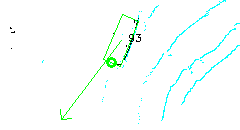
\includegraphics[width=0.5\textwidth]{bilder/obst_rot.png}
\label{obst_rot}
\end{center}
\end{figure}

% Basierend auf der Bewegungrichtung wird nun die Ausrichtung des Fahrzeiges berechnet. Dazu werden alle dem Objekt zugewiesenden Cluster zusammengefasst und um $-\theta$ gedreht.
% Danach wird das Objekt wird in 3 gleich große Segmente unterteilt (\cref{obst_devide}).

Based on the direction of movement, the alignment of the vehicle is now calculated. To do this, all clusters assigned to the object are grouped together and rotated by $-\theta$.
Then the object is divided into 3 equal sized segments (\cref{obst_devide}).

\begin{figure}[!ht]
\begin{center}
\caption{Obstacle Cutting}
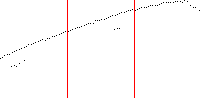
\includegraphics[width=0.5\textwidth]{bilder/obst_devide.png}
\label{obst_devide}
\end{center}
\end{figure}

% Weiterhin wird bestimmt ob sich das Objekt oberhalb oder unterhalb der x-Achse befindet. Dies ist wichtig, da wir wissen müssen, welche seite des Objekts wir messen.
% Befindet sich das Objekt aso unterhalb der x-Achse wird im nächsten Schritt der y-Wert maximiert, befindet es sich oberhalb, wird er minimiert.
% Im folgenden gehen wir davon aus, dass sich das Objekt unter der x-Achse befindet. Deshalb maximieren wir nun im linken und rechten Segment des Geteilten
% Hindernises die y-Werte. Die Unterteilung in 3 Segmente ist nötig um zu verhindern, das beide Maxima in den selben Punkt laufen und der Abstand bdier Punkte nciht zu klein wird,
% was eine größe ungenauigkeit verusachen würde. Mit diesen Punkten $(\vec{R};\vec{L})$ wird nurn eine korrektur der Drehung des Objektes berechnet:

It is also determined whether the object is above or below the x-axis. This is important because we need to know which side of the object we are measuring.
If the object is below the x-axis, then the y-value is maximized in the next step; if it is above, it is minimized.
In the following, we assume that the object is under the x-axis. Therefore we maximize the y-values in the left and right segment of the divided obstacle.
The division into 3 segments is necessary to prevent the two maxima from running into the same point and the distance of the points doesn't become too small, 
which would cause a great inaccuracy. With these points $(\vec{R};\vec{L})$ (\cref{obst_correction}) a correction of the rotation of the object is now calculated:




\begin{align*}
\Delta x &= R_x - L_x\\
\Delta y &= R_y - L_y\\
\theta_{correction} &= \atantwo(\Delta y,\Delta x)
\end{align*}


\begin{figure}[!ht]
\begin{center}
\caption{$\theta$ - Correction}
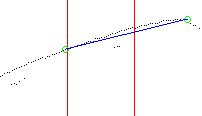
\includegraphics[width=0.5\textwidth]{bilder/obst_devide_angle.png}
\label{obst_correction}
\end{center}
\end{figure}

% Nach Anwendung der Korrektur wird die größe des Hindernises berechnet. Dazu werden die maximalen und minimalen x und y Werte des erneut um $\theta_{correction}$ gedrehten Onjektes herangezogen.
% Mit diesen Werten wird nun über die Zeit ein auf 0.5m gerundetes Histogram für die Länge und Breite des Hindernises aufgebaut.
% Anhand diesem wird dann der warscheinlichste Wert ausgewählt. Dadurch ändert sich die Größe des Hindernisses zu begin häufiger,
% bevor die Größe auf einen stabilen wert konvergiert.Da die größe des Objekts zu begin sehr klein sein kann, 
% gibt es für beide Werte einen unteren Grenzwert von 0.9m . Messerte für ein Beispielobjekt sind in \cref{obst_hist} zu sehen.

After applying the correction, the size of the obstacle is calculated. For this purpose, the maximum and minimum x and y values of
rotated objects are used. With these values, a histogram for the length and width of the obstacle, rounded to 0.5 m, is now established over time. \todo{warum 0.5m??}
The most probable value is then selected. This causes the size of the obstacle to change more often before the size converges to a stable value.
Since the size of the objectat the begin can be very small, there is a lower limit of 0.9m for both values. Measured values for a sample object can be seen in \cref{obst_hist}.
\begin{figure}[!ht]
\begin{center}
\caption{Object Size Histogram}
\begin{tikzpicture}
\begin{axis}[ylabel={number of measurements},ybar interval, ymax=366,ymin=0,xmin=0.7,xmax=6.8, minor y tick num = 3,
width=0.54\textwidth,
height=0.6\textwidth]
\addplot[fill=gray!50] coordinates { (1.0, 29) (1.5, 58) (2.0, 366) (2.5, 35) (3.0, 3) (3.5, 1) (4.0, 0) (4.5, 0) (5.0, 0) (5.5, 0) (6.0, 0) (6.5, 0) };
\end{axis}
\begin{axis}[ybar interval, ymax=366,ymin=0,xmin=0.7,xmax=6.8, minor y tick num = 3,
width=0.54\textwidth,
height=0.6\textwidth,
at={(0.48\textwidth,0)}]
\addplot[fill=gray!50] coordinates { (1.0, 0) (1.5, 0) (2.0, 7) (2.5, 6) (3.0, 9) (3.5, 2) (4.0, 64) (4.5, 84) (5.0, 318) (5.5, 3) (6.0, 2) (6.5, 2) };
\end{axis}
\node at (0.21\textwidth,0.5\textwidth) {width[m]};
\node at (0.7\textwidth,0.5\textwidth) {length[m]};
\end{tikzpicture}
\label{obst_hist}
\end{center}
\end{figure}

% Leicht zu sehen wird für das Object eine breite von 2m und eine Länge von 5m berechnet. Das Objektist in diesm Fall ein Volvo S60, welcher Außenmaße von ca. 1.9m und 4.6m hat,
% womit die Abweichungen sich korrekt innerhalb, der Rundung der Werte befinden. Für die Nachfolgende filterung der Messwerte mit Hilfe eines Kalman filters, wurd nun
% die Position des Fahrzeuges aus dem Mittelpunkt der Boundingbox bestimmt.

Easy to see, a width of 2m and a length of 5m is calculated for the object. In this case the object is a Volvo S60, which has outer dimensions of approximately
1.9m and 4.6m, whereby the deviations are correctly within, the rounding of the values. 
It can be seen that the distribution of the width, is similar to a normal distribution, which is due to the fact that the rotation of the object has a noise.
In the case of length, however, we see that the algorythm tends to calculate to small values, which results from the fact that this can only be inadequately
measured when the vehicle is moving towards the sensor. Because to the internal vehicle structure, the sensor is not able to see through the vehicle, so the
values are to smal.

For the subsequent filtering of the measured values with the help of an extended Kalman filter, 
the position of the vehicle from the center of the bounding box is now determined, using the mean value of the four corner points

% Die für die Berechnung der Bewegungsrichtung genutzte Position ist jedoch eine andere, da die so eben berechnete Position zu diesem Zeitpunkt noch nicht zur verfügung steht und
% die Position kurz nach der Initialen erkennung durch die häufigen Größenändrungen sehr instabil ist. Deswegen wird als Position immer die maximale x-Koordinate der Cluster gesnutzt.
% Diese Postition kann ebenfalls in \cref{obst_rot}, als kleiner grüner Kreis begutachtet werden.
% Da $\theta$ im initialen Zeitschritt Null ist, entpricht dies der globalen Maximalen x-Koordinate des Clusters. Dies Führt dazu, das wir im Initialen Zeitschritt annhemen, dass sich das Objekt
% in die positive x-Richtung bewegt. Bei Objekten bei denen das nicht der Fall ist, führt das zu einem kurzzeitigen oszillieren der Orientierung, welche sich jedoch über die Zeit schnell stabilisiert.

However, the position used for the calculation of the direction of movement is different, since the so calculated position is not yet available at this time 
and the position is very unstable shortly after the initial recognition due to the frequent dimensional changes. Therefore, the maximum x coordinate
of the rotated clusters is always used as the position. This position can also be examined in \cref{obst_rot}, as a small green circle. Since $\theta$ in the initial time step is zero, 
this corresponds to the global maximum x-coordinate of the cluster. This leads to the assumption that the object moves in the positive x direction in the initial time step. 
For objects where this is not the case, this leads to a short-term oscillation of the orientation, which however quickly stabilizes over time.

% Der eine oder ander möge sich wundern warum die Boundingbox so aufwendig berechnet wurde. Eine Einfache Art und weise eine Boundingbox für die Objekte zu berechnen wäre die berechnung
% der Minimum Boundingbox über die konvexe Hülle, so wie es in vielen Anderen Arbeiten gemacht wird \cite{Zhang,Himmelsbach2009}. Die Minimum Bounding box liefet jedoch unter umständen nicht das gewünschte
% ergebnis, zum einen hat man die immer nur die größe der aktuellen Messung und zum anderen kann sie eine falsche Orientierung liefern, wie in \cref{min_box} zu sehen.

One thing or another may be wondering why the Boundingbox was calculated so elaborately. A simple way to calculate a bounding box for the
objects would be the calculation of the minimum bounding box over the convex hull, as it is done in many other works \cite{Zhang, Himmelsbach2009}.
The minimum Bounding box, however, under certain circumstances does not provide the desired result, on the one hand you have only the size of the current measurement and on the 
other hand it can provide a wrong orientation as seen in \cref{min_box}.

\begin{figure}[!ht]
%\begin{center}
\caption{Error with minimum Boundingbox \cite{Himmelsbach2009}}
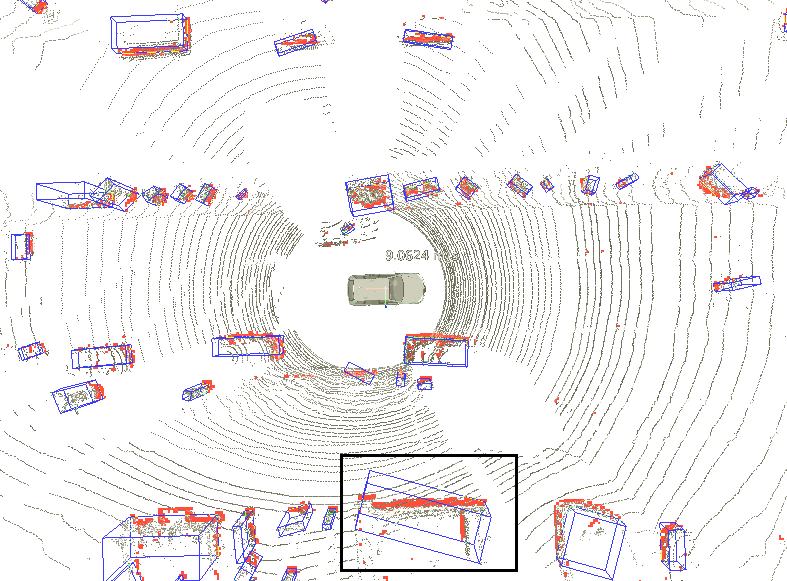
\includegraphics[width=\textwidth]{bilder/min_bound.png}
\label{min_box}
%\end{center}
\end{figure}

% Da die orientierung und Postition der Objekte jedoch als eingang für den nachfolgenden Kalmanfilter genutzt wird, welcher sehr sensible auf falsch Orientierungen reagiert, wurde eben jeder Algorithmus
% entwickelt.

However, since the orientation and position of the objects are used as input for the subsequent Kalman filter, which reacts very sensitively to false orientations, the algorithm was developed.

\subsection{Object Confidence}
% Um zu verhindern, dass kurzzeitig erkannte False Positives direckt als Objekt erkannt werden und damit die nachfolgende Logik beeinflusst, wird nun ein Confidence Wert eingeführt
% Bevor ein erkanntes Objekt als gültig erachtet wird, muss dieses einen gewissen Confidence Wert erreichen. Der Initiale Konfidence Wert eines Objektes ist Null. Der Konfidence wert
% wird um eins erhöht, wenn das Objekt in zwei aufeinader folgenden Zeitschritten getrackt werden kann und folgende bedingungen erfüllt: 

In order to prevent the detection of false positives immediately recognized as an object and thus to influence the subsequent logic, a confidence value is now introduced. 
Before a recognized object is considered to be valid, this must achieve a certain confidence value. The initial confidence value of an object is one. 
The confidence value is increased by one if the object can be tracked in two consecutive time steps and satisfies the following conditions:

\begin{itemize}
\item The width of the object must be less than the length of the obstacle plus 1.5m
\item The length of the obstacle must be less than 10m
\item The width of the obstacle must be less than 4m
\end{itemize}
% Ist eine dieser Bedingunggen nicht erfüllt, wird der Confidence Wert statdessen halbiert. Damit ein Objekt als gütig erachtet wird, muss es einen Confidence wert von 3 erreichen, sodass
% Ein Objekt erst nach mindestens 3 drei Iterationen erkannt werden kann.
If one of these constraints is not met, the Confidence value is halved. For an object to be considered kind, it must reach a confidence value of three so that an object can only be 
recognized after at least two iterations. This value was empirically determined and represents a tradeoff between fast detection and filtering.


\section{Classification}
\todo{implementierung Plausibilitätstest}
% Nun wird eine  Klassifizierung der Objekte anhand ihrer Größe vorgenommen, es findet keine Klassifizierung nach bewegten und unbewegten Objeten Stadt.
% Unterschieden werden lediglich Fußgänger, Radfahrer, und Fahrzeuge, und Sonstige. Als Klassifizierungs kritterium wird die Größe der Onjekte genutzt.
% Die Klassifizierung sieht wie folgt aus:
Now a classification of the objects is made by their size, there is no classification according to moved and immobile objects.
Only pedestrians, cyclists, vehicles, and others are differentiated. The size of the objects is used as a classification criterion.
The classification is as follows:
\begin{description}
\item[pedestrian:] length < 1.5 and width < 1.5
\item[cyclist:] length < 2 and width < 1.5
\item[car:] length < 10 and width < 4
\item[undefined:] length >= 10 and width >= 4
\end{description}

% Objekte die eine Größe von 2x1.5m überschreiten werden dabei als Fahrzeug Klassifiziert, Objekte die kleiner als 1.5x1.5m sind werden als Fußgänger klassifiziert. Alles dazwischen wird als Radfahrer klassifizierfiziert.
% Weiterhin wird andhand der Geschwindigekeit eine Plausibilitätstest durchgeführt. So darf eine Fußgänger eine Geschwindigekeit von 10km/h nicht überschreiten und die Maximalgeschwindigkeit dür einen 
% Radfahrer bertägt 30km/h. Da für Fahrzeuge keine sinnvolle geschwindigkeitsgrenze angenommen werden kann, wir an ihrer stelle die Änderung der Orientierung genutzt. Als Maximale Drehrate wird
% eine Messung von 0.3 rads/sec aus \cite{Kelly1994} angenommen. Da der Wert eine Obere Grenze darstellen soll nehmen wir einen etwas höheren  Wert von  0.3 rads/sec an. Wird einer dieser Werte überschritten,
% wird der Confidence ebenfalls halbiert.

Furthermore, a plausibility test is carried out using the speed. Thus, a pedestrian must not exceed a speed of 10km/h and the maximum speed for a cyclist is 30km/h.
Since no sensible speed limit can be assumed for vehicles, we use the change of orientation in their place.
The maximum rotation rate is assumed to be 0.1 rads/sec from \cite{Kelly1994}. Since the value is an upper limit, we assume a slightly higher value of 0.2 rads/sec.
If one of these values is exceeded, the confidence is also halved.


% \begin{lstlisting}[language=Python]
% if length < 1.5 and width < 1.5:
%     type = pedestrian
%     
% elif length < 2 and width < 1.5:
%   type = cyclist
%   
% elif length < 10 and width < 4:
%     type = car;
% else:
%   type = undefined
% \end{lstlisting}


\section{State Estimation}

% Nachfolgende des Trackings wird auf den Erkannten Objekten eine Zustandschätzung durchgeführt. Dies ist nötig, da Objekte während der Fahrt verdenkt werden können,
% sei es durch andere bewegte Objekte oder Gebaüde. Eine schätzung des Zustandes über den Erkennungshorizont hinaus erlaubt es uns eine Aussage über die Position von
% Objekten zu treffe, welche im Moment nicht sichtbar sind. Weiterin erlaubt es auf einfache Weise zeitweise nicht erkannte Objekte wiederzuerkennen, also dem Objekt
% die gleich ID zuzuweisen wie zuvor. 
Following the tracking, a state estimation is performed on the detected objects. This is necessary because objects can be hidden during the movement,
be it by other moving objects or buildings. An estimation of the state beyond the detection horizon allows us to make a statement about the position of 
objects which are not visible at the moment. Furthermore, it allows you to easily redetect objects that have not been detected at a time, ie to assign the same ID to the object as before
and allows a well filtering of the measured objects.

% Aus dem zuvor durchgführten Tracking können wir die Aktuelle Position, Geschwindigekeit, Drehung und Drehgeschwindigkeit erhalten. 
% Für eine Zustandschätzung mit den für Fahrzeuge üblichen Bicycle Model fehlen \todo{reference} und Angangen über den Radstand und Gewicht des Fahrzeues.
% Daher müssen wir uns auf ein relativ Einfaches ``Constant Turn Rate and Velocity'' Model beschränken. Dies erlaubt es uns allerdings das gleiche
% Model für alle Klassen von Objekten zu nutzten. Da dieses Model ebenfalls auf Fußgänger und Radfahre angewendet werden kann.

From the previous tracking, we can get the current position, speed, rotation and rotation speed. For an estimation of the state with the for vehicle common the bicycle model \cite{althoff2014online,snider2009automatic,kong2015kinematic}, 
we miss the wheelbase and the weight of the vehicle. Therefore, we must limit ourselves to a relatively simple ``Constant Turn Rate and Velocity'' model.
This allows us to use the same model for all classes of objects. Because this model can also be used on pedestrians and cyclists.

\subsection{Constant Turn Rate and Velocity Model}
The state vector \cite{Schubert2008} of the CTRV model looks as follows:
\begin{align*}
\vec{x}(t) &=
\begin{bmatrix}
x & y & \theta & v & \omega
\end{bmatrix}^T\\
x &\text{ - X Axis}\\
y &\text{ - Y Axis}\\
\theta &\text{ - Object Yaw Angle}\\
v &\text{ - Object Velocity}\\
\omega &\text{ - Yaw Rate}
\end{align*}

The dynamic matrix is obtained by a non-linear state transition:

\begin{align*}
f = \vec{x}(t + \Delta t)=
\begin{bmatrix}
\frac{v}{\omega} (-\sin(\theta) + \sin(\Delta t \omega + \theta)) + x(t) \\
\frac{v}{\omega} (\cos(\theta) - cos(\Delta t \omega + \theta)) + y(t) \\
\omega \Delta t + \theta\\
v\\
\omega
\end{bmatrix} 
\end{align*}

% Da es sich beid er Dynamikmatrix um einen nichtlinearen Zustandsübergang handelt benötigen wir noch die Jacobi Matrix.
% Diese wurde auf Grund ihrer Göße eingekürzt.
%Die Matrix wure mit Sympy generiert, und auf Grund ihrer Größe eingekürzt.
Since the dynamics matrix is a non-linear state transition, we still need the Jacobian matrix. This was shortened because of its size.
 
 
\begin{align*}
J(\vec{x})=
\begin{bmatrix}
1 & 0 & \frac{v}{\omega} (-\cos(\theta) + \cos(\Delta t \omega + \theta))& \dots & \dots \\
%\frac{1}{\omega} (-\sin(\theta)) + \sin(T \omega + \theta)& multi-body simulation
%\frac{Tv}{\omega} \cos(T \omega + \theta) - \frac{v}{\omega^2}(-\sin(\theta) + \sin(T\omega + \theta) 
0 & 1 & \frac{v}{\omega} (-\sin(\theta) + \sin(\Delta t \omega + \theta))& \dots & \dots \\
0 & 0 & 1 & 0 & \Delta t\\
0 & 0 & 0 & 1 & 0\\
0 & 0 & 0 & 0 & 1
\end{bmatrix} 
\end{align*}


\subsection{Extendet Kalman Filter}


% Der Extendet Kalman Filter (EKF) ist die nichtlineare Version des Kalman-Filters, die sich über eine Schätzung des aktuellen Mittels und der Kovarianz linearisiert.
% Zusätlich zu unserem Modell werden noch weitere Werte benötigt. Dazu zehen wir uns die Berechnungsforschrift an:

The Extendet Kalman Filter (EKF) \cite{Ribeiro2004} is the nonlinear version of the Kalman filter, which is linearized by an estimate of the current mean and the covariance.
In addition to our model, further values are required. For this purpose, we look at the calculation rules of the necessary steps.

\subsubsection{Prediction}

In the first step of the filtering process, the preceding estimation of the state dynamics is projected to a prediction for the current time.

\begin{align*}
\hat{x}_{k} &= f(\hat{x}_{k-1},u_{k-1})\\
P_{k}&=F_{k-1} P_{k-1} {F^T_{k-1}} + Q_{k-1}
\end{align*}

Where $\hat{x}_{k}$ is the estimate of our state for the current time step and $P_{k}$ is, because of the prediction, our increased covariance.

% with:
% \begin{itemize}
%  \item $f$ - state transition
%  \item $\hat{x}$ - estimated state
%  \item $u$ - control vector
% \end{itemize}

Since we can not know the control variables of the other objects, we asume $u$ to be zero for our calculations.
For the state transition model $F$ we use our previous calculated Jacobian matrix applied to the previous state.

\begin{align*}
\hat{x_{k}} &= f(\hat{x}-{k-1},0)\\
P_{k}&=J_{k-1} P_{k-1} {J^T_{k-1}} + Q_{k-1}
\end{align*}

% Für die Process Noise Covariance Matrix $Q$ nehmen wir als ausgangspunkt typische worst case werte für Fahrzeuge aus \cite{Kelly1994} an.
% maximum acceleration: $a = 8.8 \frac{m}{s^2}$, maximum turn rate: $\omega = 0.1 \frac{rad}{s}$,   maximum turn rate acceleration: $\dot\omega = 0.1 \frac{rad}{s^2}$
% Diese Werte werden dann integriert, bis die Einheit korrekt ist. Abschliend, da wir eine Varianz haben wollen werden die Werte quadriert.

For the Process Noise Covariance Matrix $Q$, we assume typical worst case values for vehicles from \cite{Kelly1994} as the starting point,
maximum acceleration: $a = 8.8 \frac{m}{s^2}$, maximum turn rate: $\omega = 0.1 \frac{rad}{s}$,   maximum turn rate acceleration: $\dot\omega = 0.1 \frac{rad}{s^2}$.
These values are then integrated until the unit is correct. Finally, since we want to have a variance, the values are squared. 
We assume no correlation between all other values and get only values in the main diagonal.

\begin{align*}
Q=
\begin{bmatrix}
(\frac{a \cdot \Delta t^2}{2})^2 & 0 & 0 & 0 & 0\\
0 & (\frac{a \cdot \Delta t^2}{2})^2 & 0 & 0 & 0\\
0 & 0 & (\omega \cdot \Delta t)^2 & 0 & 0\\
0 & 0 & 0 & (a \cdot \Delta t)^2 & 0\\
0 & 0 & 0 & 0 & (\dot\omega \cdot \delta t)^2
\end{bmatrix} 
\end{align*}

% sGPS     = 0.5*8.8*dt**2  # assume 8.8m/s2 as maximum acceleration, forcing the vehicle
% sCourse  = 0.1*dt # assume 0.1rad/s as maximum turn rate for the vehicle
% sVelocity= 8.8*dt # assume 8.8m/s2 as maximum acceleration, forcing the vehicle
% sYaw     = 1.0*dt # assume 1.0rad/s2 as the maximum turn rate acceleration for the vehicle
% 
% Q = np.diag([sGPS**2, sGPS**2, sCourse**2, sVelocity**2, sYaw**2])

% Weiterhin wurden  mussten in diesem Schritt eineige optimierungen gemacht werden um die nummerische stabilität zu gewährleisten.
% Fällt die Drehrate auf einen sehr niedrigen wert, riskieren wir eine Division durch null. Um diesn fall abzufangen, wurde
% ein neuer Zustandsübergang definiert:
Furthermore, some optimization had to be made in this step in order to ensure the numerical stability. 
If the yaw rate is very low, we risk a division by zero. In order to except this situation, a new state transition was defined,
in which we ignore the direct influence of the yaw rate on the position, when it falls below a value of $0.0001\frac{rad}{s}$. 
The resulting error is very small, since the yaw rate is close to zero.
% \todo{wodurch unterscheidet sich die vereinfachte state transition
% es ist gut dargestellt WARUM du die vereinfachung machst
% aber was die physikalisch bedeutet könnte man noch klarer darstellen}

\begin{align*}
f = \vec{x}(t + \Delta t)=
\begin{bmatrix}
v \cdot \Delta t \cdot \cos{\theta}+ x(t) \\
v \cdot \Delta t \cdot \sin{\theta}+ y(t) \\
\theta + \Delta t \cdot \omega\\
v\\
\omega
\end{bmatrix} 
\end{align*}

The corresponding Jacobian matrix is then:
\begin{align*}
J(\vec{x})=
\begin{bmatrix}
1 & 0 & -\Delta t \cdot v \sin{\theta} & \Delta t \cdot \cos{\theta} & 0\\
0 & 1 & \Delta t \cdot v \cos{\theta} & \Delta t \cdot \sin{\theta}  & 0\\
0 & 0 & 1 & 0 & \Delta t\\
0 & 0 & 0 & 1 & 0\\
0 & 0 & 0 & 0 & 1
\end{bmatrix} 
\end{align*}



\subsubsection{Updating}
\todo{correction step EKF näher beschreiben
da der nicht standard im ekf is
was machst du mit statevector
(wohl nur werte überschreiben)
was machst du mit uncertainty
so den state estimation teil hab ich durchgelesen
}

The predictions are finally corrected with the new information of the measurements.

\begin{align*}
\tilde{y}_k &= z_k -h(\hat{x}_{k})\\
S_k &= H P_k H^T_k + R_k\\
K_k &= P_k H^T_k S_k^{-1}\\
\hat{x}_k &= \hat{x}_k + K_k \tilde{y}_k\\
P_k &= (I - K_k H_k) P_k
\end{align*}


Since we directly measure all states of our system there is observation function for our measurements, means our
$h(\hat{x}_k)$ equals $\hat{x}_k$. Because of this our observation matrix $H$ results in a simple Identity matrix.

For the Measurement Noise Covariance Matrix $R$ we assume experimental determined values. Since we are quite sure about the position we
assume a small value of 1 and a value of 0.1 for the rotation, for the same reason. For the velocity we chose a quite high value of 4,
because it is derived from the position over time. The same for the yaw rate with a value of 0.1. Again we assume no correlation between all other values,
which it is most likely not true, but would need more further investigation.

\begin{align*}
R=
\begin{bmatrix}
1 & 0 & 0 & 0 & 0\\
0 & 1 & 0 & 0 & 0\\
0 & 0 & 0.1 & 0 & 0\\
0 & 0 & 0 & 4 & 0\\
0 & 0 & 0 & 0 & 0.1
\end{bmatrix} 
\end{align*}



% \begin{itemize}
%  \item $h$ - predicted measurement transformation
%  \item $z$ - measurements
%  \item $u$ - control vector
%  \item $H$ - observation matrices
% \end{itemize}


% In diesem Schritt des Filters muss beachtet werden, dass wir mir Rotationen arbeiten die im Bereich von $[-180 \le \theta \le 180]$ definiert sind und desshalb Singularitäten auftreten können.
% Da unsere Messdaten verraucht sind , kann es vorkommen, dass unser State bei 179 Grad ist und mit einem Wert von $-179$ geupdatet werden soll. Nehmen wir der einfachheit an,
% dass beide werte gleich gewichtet sind, ergibt sich nach dem update ein Wert von 0 Grad, dies ist offensichtilich falsch. Deshalb, wird vor jedem updateschritt bei bedarf
% $360$ Grad addiert oder suptrahiert, do das der Abstand zwischen State und Messwert minimert wird. Nach dem Updae wird der interne State wieder auf den bereich $[-180 \le \theta \le 180]$ normiert.
% Betrachten wir nun wieder unser Beispiel mit den korrigierten Werten, State: $179-360=-181$ Grad und Messwert: $-179$ Grad erhalten wir den korrekten Wert von $-180$ Grad.

In this step of the filter it must be noted that we are working with $\theta$ that is defined in the range of $ [- 180^{\circ} \le \theta \le 180^{\circ}] $ and therefore singularities can occur.
Because our measurement data is noisy, our state may be at 179 degrees and is updated with a value of $ -179^{\circ} $. For the sake of simplicity we assuming that both values are equally weighted,
the update step results in a value of 0 degrees, which is obviously wrong. Therefore, before each updating step, $ 360 $ degree is added or suptracted,
so the distance between state and measured value is minimized. After updating, the internal state is again normalized to the range $ [- 180^{\circ} \le \theta \le 180^{\circ}] $.
Consider now again our example with the corrected values, state: $ 179-360 = -181 $ degree and measured value: $ -179 $ degree, we get the correct value of $ -180 $ degree.


\subsubsection{Initial Uncertainties}

% Unsere Initale Covariance Matrix $P$ wurde ebenfalls expirimentel ermittelt. Für die Postition nehmen wir, da wir sie direckt messen können, eine hohe sicherheit an, und setzten 
% diese auf eins. Da wir die Rotoation ebenfalls direckt mess nehmen wir einen wert von 0.1 an. Da wir die zeitabhängiugen größen im ersten schritt nicht messen können,
% wird hier einsehr hoher Wert von 1000 angesetzt.
Our initial covariance matrix $ P $ was also determined expirimentel. For the position we take a high degree of safety, since we can measure them directly, and put them on one. 
Since we also measure the rotoation directly we take a value of 0.1. Since we can not measure the time-dependent variables in the first step, a very high value of 1000 is chosen here.

\begin{align*}
P_{initial}=
\begin{bmatrix}
1 & 0 & 0 & 0 & 0\\
0 & 1 & 0 & 0 & 0\\
0 & 0 & 0.1 & 0 & 0\\
0 & 0 & 0 & 1000 & 0\\
0 & 0 & 0 & 0 & 1000
\end{bmatrix} 
\end{align*}



\subsection{Reassigning}
% Befindet sich ein Objekt innerhalb der Rechihweite des Velodyne Sensors und wird im Darauffolgenden Zeitschritt nicht erkannt,
% wird der Prediktionsschritt des Kalman filter weiterhin ausgeführt. Dies geschieht solange die Unsicherheit der Position einen gewissen \todo{konkretisieren schwellwert} Schwellwert üerschreitet.
% Sollte eine dieser Bedingungen nicht zutreffen, wird das Objekt aus der Liste der bekannten Objekte entfernt. Sobald das Clustertracking dann ein neues Objekt detektiert,
% dem keine Bisher bekannte ID zugewiesen werden kann, wird die Postion mit allen Onjekten in der Prediktionsphase
% abgeglichen. Befindet sich das neue Objekt nahe an der predizierten Position wird der Cluster dem Onjekt zugewiesen, und der Korrekturschritt des EKF durchgeführt.

If an object is within the range of the Velodyne sensor and is not detected in the subsequent time step, the prediction step of the Kalman filter is still executed.
This is done as long as the confidence value of the object does not reach zero. As soon as the cluster tracking detects a new object which can not be assigned a previously known ID,
the position is matched with all objects in the prediction phase. If the new object is within three meters to the predicted position, the cluster is assigned to the object
and the correction step of the EKF is performed. If more than one object matches these condition the closest object is assigned.

\chapter{Simulation}
% Die Simulationsumgebeung, welche verwendet wird ist VREP \footnote{\url{http://www.coppeliarobotics.com/}}. VREP wurde für verschiedenne Robottikanwendungen entwickelt.
% VREP erlaubt es innerhalb eines Graphischen beliebige \ac{MKS}, basierend auf diversen Physikengines zu konstruieren. Weiterhin verfügt VREP bereits über
% viele fertige Sensormodell, wie beispielsweise den Velodyne VLP-16. Die ganze Simulation kann über ein RemoteAPI Interface mit nahezu jerder Programmiersprache kommunizieren.

The simulation environment being used is VREP \footnote{\url{http://www.coppeliarobotics.com/}}. VREP has been developed for various robotic applications.
VREP allows you to construct any \ac{MKS} based on various physicsgines within a graphic editor. Furthermore, VREP already has many ready-to-use sensor models, such as
the Velodyne VLP-16. The whole simulation can communicate via a RemoteAPI interface with nearly every programming language.



\section{Simulation Scenario}


\begin{figure}[!ht]
%\begin{center}
\caption{VREP}
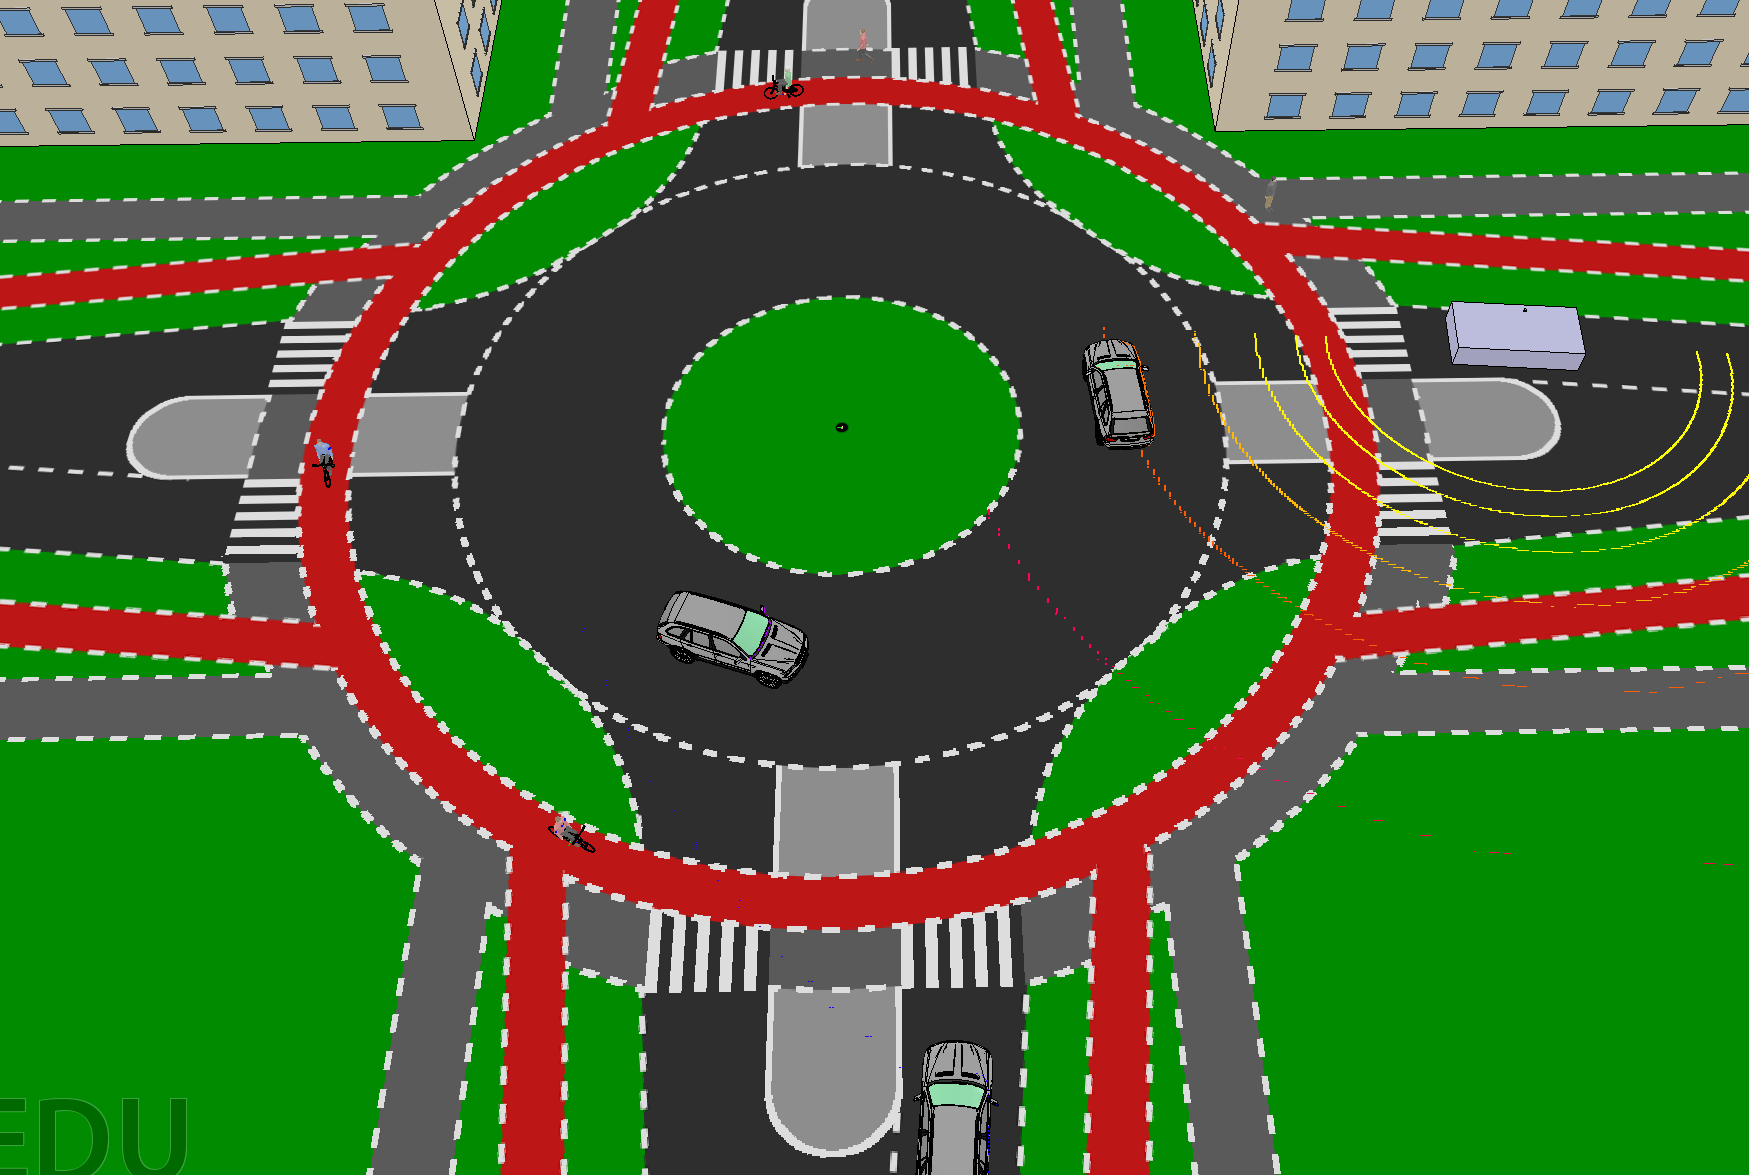
\includegraphics[width=\textwidth]{bilder/scenario.png}
\label{vrep}
%\end{center}
\end{figure}




\todo{referenzen zu ``roundabout in law'' mit formelsymbolen und so}
% Für Das Simalations Scenario wurde eine einfacher kleiner Kresiverkehr mit einem Außendurchmesser von 26m und ein Minikreisverkehr designt, da dies auf grund seiner größe 
% in Kombination mit dem VLP-16, welcher in diesem Bereich noch eine akzeptable auflösung verfügt, das interessanteste Objekt darstellen.
% Und im Innerstätischen Bereich auf grund ihrer größe haufig anzutreffen sind. Zum testen der Onjektdetektion bietet der Kleine Kreisverkehr auf Grund seiner bebaubaren
% mittelinsel gute möglichkeiten das Tracking zu testen. Weiterhin ist es aufgrund seiner Größe möglich den kompletten Kreisverkehr zu überblicken.
% Das Ganze Senarion wurde aufgrund von limitierungen in Vrep um den Faktor 10 herunterscaliert.

For the simulation scenario, a simple small roundabout with an outside diameter of 30m, according to the rules in \cite{man06} was designed. According this the cycle path must have a minimum distance of 4 m to the road and
the lane width of the circular driveway and circular exit sould be 3.75m. The recommended corner rounding radius is according to \cite{man06} 12m.

The small roundabout was chosen because this is the most interesting object due to its size in combination with the VLP-16, which still has an acceptable resolution in this area.
And in urban areas due to their size, they are frequent. Furthermore, due to its size, it is possible to survey the entire roundabout. The whole scenario was down-scaled by a factor of 10 due to limitations in Vrep.

% Innhrhalb des Szenarosn bewegen sich innerhalb des Kreisverkehrs ein Fahrad, ein Fußgänder und ander 2 Fahrzeuge. Die Objekte bewegen sich dabei auf festgelegten Pfaden.
% Dei Geschwindigekeit aller Verkehrsteilnehmer ist dabei auf den Typ angepasst. Der Füßgänger bewegt sichn mit für füßgänger übliche 5km/h.
% Das Fahrrad mit 15km/h. Die beiden Autos bewegen sich mit Unterschiedlichen Greschwindigkeiten zwischen 25 und 35 Km/h. Um eine Kolision der Fahrzeuge zu vermeiden, sind beide 
% Fahrzeuge an der vorderseite mit Distanzsensoren ausgestattet. Sollte dieser Sensor ein Fahrzeug erkennen, geht das Fahrzeug in eine  Adaptive Cruise Control modus und
% passt sich dem vorderen Fahrzeug an. Das Adaptive Cruise Control ist dabei als einfacher proportional regler umgesetzt.

Inside the scenario there are three bicycles, two pedestrians and three other vehicles driving around the roundabout. The objects are moving on fixed paths.
The speed of all traffic is adapted to the type. The pedestrian moves with the 5km/h usually asumed for pedestrians.
The bike with 15km/h. The two cars move at different speeds between 25 and 35 km/h. In order to avoid a collision of the vehicles,
both vehicles are equipped with distance sensors at the front. If this sensor detects a vehicle, the vehicle enters an \acl{ACC} mode and adapts to the front vehicle.
The Adaptive Cruise Control is implemented as a simple proportional controller.

% Das autonome Fahrzeug bewegt sich dabei ebenfalls auf eine festen Pfad, dieser führt von rechts in den Kreisverkehr ein und verlässt den Kreisverkehr an der dritten ausfahrt.
% die Aufgabe des Fahrzeues ist dabei sich sicher in den Kreisfehr einzusortieren und den Kreisverkehr sicher zu verlassen. Dabei Muss das Fahhzeug sowohl aud den Fußgänger, den Radfahrer
% und die Andren Fahrzeuge innerhalb des Kreisverkehres achten. Dazu ist das Fahrzeug mit einem virtuellen Velodyne VLP-16 ausgestattet.

The autonomous vehicle also moves along a fixed path, which leads from the right into the roundabout and leaves the roundabout at the third exit. 
The task of the vehicle is to safely enter the roundabout and safely leave the roundabout. In doing so, the vehicle must pay attention both to the pedestrians,
the cyclists and the other vehicles within the roundabout. For this, the vehicle is equipped with a virtual Velodyne VLP-16 and the previously described algorithms deliver the detected objects.

\section{Simulation Logic}

% Um das zuvor beschrieben Scenario durchzuführen musste eine Logik entwicklt werden, diese umfasst nicht nur die Statemachine zum durch fahren des Kreisverkehrs, sondern
% auch die Lokalisierung des Fahrzeuges in dem Scenario als auch die Anbinung aller Sensoren an die Objekt Erkennung. Da alle nachfolgenden Berchungen nur wenig resscourcen bentigen
% wurde die entsprechende Software in Pyhon entwickelt.

In order to carry out the previously described scenario, a logic had to be developed, which includes not only the state machine for passing through the roundabout,
but also the localization of the vehicle in the scenario as well as the connection of all sensors to the object detection.
Since all subsequent calculations require little resources, the corresponding software was developed in Python.

\subsection{Sensor Connection}
% Die Objekt detection benoötigt als Sensor eingange die Daten des Velodyne VLP-16 und die Daten des Applanix POS-LV. Von den Applanix daten werden jecoch nur
% due Aktuelle Postion im WGS84 format benötigt und das aktuelle Heading. Da sich der Applanix Sensor in VREP nicht einfach nachbauen lässt,
% wird das Applanix system einfach aus den in Vrep auslesbaren Positions und Rotationsdaten generiert. Da die Position in VREP in Kartesischen Koordinaten
% angeben ist, werden dies über die in OpenDAVINCI enhaltene Transformation anhand einer Referenzkoordinate in WGS84 Koordinaten transformiert.
The object detection requires the data of the Velodyne VLP-16 and the data of the Applanix POS-LV as sensor input.
However, only the current position in the WGS84 format and the current heading are required by the object detection.
Since the Applanix sensor can not be easily reconstructed in VREP, the necessary data is simply generated from the position and rotation data readable in Vrep.
Since the position in VREP is specified in Cartesian coordinates, they are transformed via the transformation contained in OpenDAVINCI, using a reference coordinate in WGS84 format.

% Die Anbindung des Velodyne VLP-16 gestaltet sich schwieriger, da der Aufabau der Messdaten sich signifikant vom Originalvelodyne unterscheidet.
% Zwar werden die Daten ebenfalls in Polarkoordinaten ausgegeben, jedoch werden nur Messwerte ausgegen, wenn diese auf ein Onjekt treffen. Da ein Großteil des Scenarios leerer Raum ist
% weisen die Messdaten viele löcher auf, wesshalb diese in eine geeignete Form transformiert werden müsssen.
The connection of the Velodyne VLP-16 is more difficult because the structure of the measured data differs significantly from the original Velodyne.
Although the data is also output in polar coordinates, only measured values are output when they hit an object. Since a large part of the scenario is empty space,
the measurement data have many holes on them. But the object detection needs continuous measurements, so they must be transformed into a suitable form.

% Dabei ist zu beachten, das das Onjekttracking eine vollständige 360 Gram Messung erwartet, dazu muss zusätzlich gewartet werden, bis alle Nötigen Messdaten vorliegendn.
% Der virtualle Velodynle liefet eine Messrate von 10Hz, und ist dabei in 4 Segmente eingeteilt, welche nacheinander ausgelesen werden. Der zur simulation verwendete Zeitschritt
% beträgt 50ms, so dass wir 2 Segemente in einem Zeitschritt auslesen können. Solbald alle Daten gesammelt sind, werden diese zu einem geeigneten Messframe zusammengesetzt.
It is important to note that object detection requires a complete 360 degree measurement. To do this, you must wait until all necessary measurement data are available.
The virtualle Velodynle runs a measuring rate of 10Hz, and is divided into 4 segments, which are read one after the other. 
The time step used for the simulation is 50 ms, so that we can read out 2 segments in one step. Once all data are collected, they are assembled into a suitable measuring frame.

% Die glieferten Messdaten liegen als liste von Kugelkoordinaten vor (Radius $r$, Polarwinkel $\theta$, Azimutwinkel $\Phi$). Da die Azimut und Polarwinkel dabei nicht in Aquidistanzen Abständen
% vorliegen, jedoch eine sehr viel höhere Auflösung als der originale Sensor haben, werden die Messwerte auf die Originale auflösung von 0.2 bzw. 2 Grad heruntergerundet und die Messerte in ein
% Entsprechendes zweidimensionales Array fester größe eingetragen eingetragen. Sodass nicht erfasste bereiche den Wert Null erhalten.

The measured data are provided as a list of spherical coordinates (radius $r$, polar angle $\theta $, azimuth angle $\Phi$).
Since the azimuth and polar angles are not at equidistant intervals but have a much higher resolution than the original sensor,
the measured values are rounded down to the original resolution of 0.2 and 2 degrees and the measured values are entered into a corresponding two-dimensional fixed-size array.
Thus, areas that are not detected have the value zero.

% Nach dem alle Erforderlichen Messdaten gesammelt und umgewandelt wurden, werden diese über ein extra entwickeltes OpenDAVINCI-Python interface an die Objekterkennung gesendet.
After all necessary measurement data have been collected and converted, they are sent to the object detection via a specially developed OpenDAVINCI-Python interface.
Unnecessary data for the Applanix is simply set to zero.

\subsection{Mapping}
% Für das Maping wird das OpenDAVINCI interne Compressed Scenario Data Format (SCNX) \cite{Berger2010} genutzt. Diese erlaubt es Szenarien zu definieren, stationären und dynamischen Elemente, 
% zu beschreiben und zu kombinieren, um unterschiedliche Verkehrssituationen zu formulieren. Das SCNX format offeriert für die Modellierung von Straßen unter anderm
% die Klassen ROAD,LANE. Wobei eien ROAD dabei aus mehreren LANE's bestehen kann. eine Lane aus einer Menge an Pukten besteht, welche den Verlauf der lane beschreiben.
% Der Lane kann weiterhin als Attribut eine Fahrspurmakierung und eine Breite zugewiesen werden. Einzelne Lanes können unterinander Verbunden werden, was mit diesen Einfachen 
% Modellen ein Komplttes Straßennetz aufgebaut werden kann. Da OpenDAVINCI kein Pythoninterface für das Parsen der Scenariofiles zur verfügungs stellt, wurde ein eigenner Lexer für die 
% VerArbeitung der Scenariofiles implementiert. Dabei wurde sich auf für die Simulation nötigen Klassen beschränkt. Daher lässt sich eine Lane sich dabei nur durch ein Punktmodell
% beschreiben, währen OpenDAVINCI zusätzlich weitere Modelle anbietet.
The OpenDAVINCI internal Compressed Scenario Data Format (SCNX) \cite{Berger2010} is used for mapping. This allows scenarios to be defined by describing and combining stationary and dynamic elements
to formulate different traffic situations. The SCNX format offers, among other things, the classes ROAD, LANE for the modeling of roads. One ROAD can consist of several LANEs.
A lane consists of a set of points which describe the course of the lane. The lane can be assigned with the attributes lane mark and width. 
Individual lanes can be connected to each other. What makes it possible to build a complicated road network with these simple models. 
Since OpenDAVINCI does not provide a Python interface for parsing the Scenariofiles, a special Lexer was implemented for the processing of the Scenariofiles. 
At thise time, only the classes required for the simulation are implemented. Therefore, a lane can only be described by a point model, while OpenDAVINCI offers additional models.

% Weiterhin musste das in OpenDAVINCI enthaltene Modell erweitert werden, da OpenDAVINCI leider keine andern Arten von wegen unterstützt.
% Daher wurde die Klasse Lane um ein Typ attribut erweitert, was es ermöglicht diese Als Rad oder Fußweg zu deklarieren.
% Der Aufbau der erweiterten Pythonklassen kann in \cref{parer_objects} begutachtet werden.
Furthermore, the model included in OpenDAVINCI had to be extended, since OpenDAVINCI unfortunately does not support other types of paths.
Therefore, the class lane has been extended by one type attribute, which makes it possible to declare this as a bicycle or footpath.
The structure of the extended Python classes can be examined in \cref{parer_objects}.

\begin{figure}[!ht]
\begin{center}
\caption{Parser Objects}
 \begin{tikzpicture} 
  \umlclass{ROAD}{
  roadid : int \\
  roadname : string \\
  lanes : lane[]}{}
  \umlclass[x=6,y=0]{LANE}{
  laneid : int \\
  width : string \\
  type : string \\
  leftlanemarking : string\\
  rightlanemarking : string\\
  pointmodell : pointmodel\\
  connections : tuple[]
  }{}
  \umlclass[x=6,y=-4]{POINTMODEL}{
  points : VERTEX2[]
  }{}
  \umlclass[x=0,y=-4]{VERTEX2}{
  points : VERTEX2[]
  }{}
  \umlunicompo[mult=1..*]{ROAD}{LANE}
  \umlunicompo{LANE}{POINTMODEL}
  \umlunicompo[mult=2..*]{POINTMODEL}{VERTEX2}
  \end{tikzpicture}
\label{parer_objects}
\end{center}
\end{figure}


% 
% Für die Handbung des Kreisverkehres musste das Kartenformat jedoch no weiter erweitert werden. Laut RASt \cite{rast06} soll ein Kreisverkehr möglichst kreisförmig sein, 
% der einfachheit halber nehmen wir für die Simulation an, dass dieser ein perfekter Kreis ist. Das heißt, dass Sowohl Straßen, Radwege und fußwege perfekt kreisförmig sind und
% duch einen inneren und äußeren Radius beschrieben werden können. Daher wurde für die Berschreibung des Kreisverkehres eine Klasse Kreisverker hinzugefügt,
% welche den Centerpunkt des Kreisverkehres, Refrenzen zu allen Lanes, und derren innere und äußere Radien enhält. Weriterhin wirden in ihm die verbindungen zu den Anschlusstraßen definiert.

For the handling of the roundabout, however, the map format had to be further extended. According to RASt \cite{rast06}, a roundabout should be as circular as possible, 
for the sake of simplicity, we assume that the roundabout in simulation is a perfect circle. This means that both roads,
cycle paths and footpaths are perfectly circular and can be described by an inner and outer radius. For this reason, a class ROUNDABOUT [\cref{roundabout_class}] was added to the description of the roundabout,
which contains the center point of the roundabout, references to all lanes, and inner and outer radii. Furthermore, the connections to the connecting lanes are defined therein.

\begin{figure}[!ht]
\begin{center}
\caption{Roundabout Class}
 \begin{tikzpicture} 
  \umlclass{ROUNDABOUT}{
  roundaboutid : int \\
  lanes : lane[]\\
  junctions : tuple[]\\
  inner\_lane\_radius : float[]\\
  outer\_lane\_radius : float[]\\
  centrum :  VERTEX2
  }{}
  \end{tikzpicture}
\label{roundabout_class}
\end{center}
\end{figure}


\subsubsection{Localization}
% Da wir uns innherlab der Simulation bewegen, können wir für die Lokalisierung eine perfekte position annehmen.
% Lokalisierung in rahmen der Karte bedeutet, das wir die aktuelle bekannte position auf ein Lanesegment mappen wollen.
% Da die lanes nur in Form von Punkten und Breite gegeben sind, werden für jeden Laneabschnitt Rechtecke berechnet und für jedes Rechteck geprüft,
% ob sich die aktuelle Postion innehalb des Rechteckes befindet. Dies wird gemacht, indem Das Rechteck (und die Position) in eine
% Achsen aligned Position gedreht und in den Koordinatenursprung verschoben wird. Weiterhin muss das Rechteck vergrößert werden, sofern wir nicht das letzte Lanesegment bearbeiten,
% da sonst eine Lücke zwischen den Rechtecken verbleiben würde. Dazu wird der Winkel zum nächsen Linienabschnitt genutzt.  Sas ganze ist in \cref{mapping} Symbolisiert.
% Wobei das blaue Rechteck das aktuell zu bearbeitende darstellt, das grüne Rechteck das nachfolgende und das orange die nötige Verlängerung
As we are within simulation, we can assume a perfect position for localization. Localization within the map means that we want to map 
the current known position to a lane segment. Since the lanes are only given in the form of points and width, rectangles are calculated
for each lane segment and the current position is checked against each rectangle.
This is done by rotating the rectangle (and the position) to an axis-aligned position and moving it to the coordinate origin. Furthermore, the rectangle must be enlarged if we
do not process the last line segment, since otherwise a gap would remain between the rectangles. For this purpose, the angle to the next line segment is used.
The whole situation is symbolized in \cref{mapping}. The blue rectangle represents the current one to be edited, the green rectangle the next and the orange the necessary extension.
\begin{figure}[!ht]
\begin{center}
\caption{Mapping Rectangles}
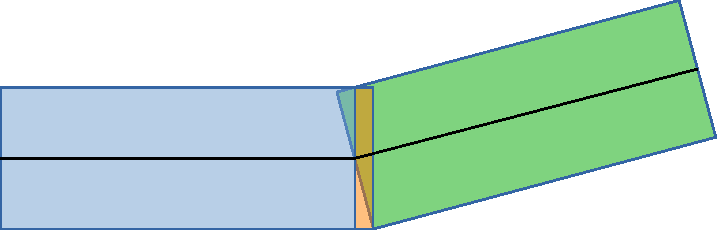
\includegraphics[width=0.7\textwidth]{bilder/mapping.pdf}
\label{mapping}
\end{center}
\end{figure}

% Wie in \cref{mapping} zu sehen, stehen die einzelnen Segmente üblicherweise nicht in einem 180 Grad winkel zueinander.
% Daher können sich die Rechtecke überschneiden und für eine Position können mehrere Rechtecke zurückgeliefert werden. In diesem Fall wird die Bewgungsrichtung des Objektes herangezogen
% und das aussicht der Bewegungsrichtung neuste Segment ausgewählt. Sollten sich mehrere Lanes überschneiden, z.B Radwege welche die Kreisverkehr einfaht kreuzen, wird 
% das richtige Segment anhand ders Objekttypes ausgewählt, also: auto -> Straße oder Radfahrer -> Radweg. Weiterhin wird die X koordinate des Objektes im gedrehten und verschobenen Koordinatensystem
% zuruckgeliefert, was für die Distanzberechnungen von nöten ist. Dabei nehmen wir immer an, dass sich das Objekt mittig auf der Spur befindet. Alternativ bietet sich für das Problem auch
% der ``Ray casting algorithm'' \cite{Galetzka2017} an. Da wir für alle Distanzberechnung annhemen, dass sich das Objekt mittig auf der Spur befindet, ergibt sich aus dieser Berechnung jedoch nur ein sehr kleiner
% Fehler und die Entfernung ergibt sich praktischer weise aus den Vorherigen Berechnungen, sodass dieser nicht umgesetzt wurde.
As seen in \cref{mapping}, the individual segments are usually not at a 180 degree angle to each other. Therefore, the rectangles can overlap and more than one rectangle can 
be returned for one position. In this case, the direction of movement from the object is used and the most recent segment of the direction of movement is selected.
If several lanes cross over, for example, cycle paths that intersect the roundabout, the correct segment is selected based on the object type, ie: auto -> road or cyclist -> cycle path.
Furthermore, the X coordinate of the object in the rotated and shifted coordinate system is returned, which is necessary for the distance calculations. We always assume that the
object is in the middle of the track. Alternatively, the `` Ray Casting Algorithm '' \cite{Galetzka2017} can be used for this problem. Since we assume for all
distance calculations that the object is in the middle of the track, this calculation results in a very small error and the distance is practically derived from the
previous calculations so that it was not applied.

\subsection{State Machine} 
% Die Statemachine ist nach Gang of Four  \cite{lester2008gang} implemetiert. Dafür wurden X \todo{nummer anpassen} States Implementiert.
% Für alle Fahrzeugeigenen berechnungen wird ein Constant acceleartion modell angenommen. Zur bestimmung der Maximalen positiven und negativen Beschleunigung
% wurden mit dem realen Fahrzeug testfahrten aufgezeichnet, bei denen die maximalen subjekiv angenehmen Werte bestimmt wurden.
The state machine is implemented according to Gang of Four \cite{lester2008gang}. For this, X States were implemented. \todo{nummer anpassen}
A constant acceleartion model is assumed for all vehicle computations. In order to determine the maximum positive and negative acceleration, 
test runs with the real vehicle  were recorded and the maximum subjectively pleasant values being determined. 

The used recordings can be seen in \cref{max_accel}, the vehicle was accelerated from 0 to 25 km/h or braked from 25 to 0 km/h.
The maximum values were read, so we assume $ 3m/{s^2} $ for the maximum positive acceleration and $ -4.5m/{s ^ 2} $ for the maximum negative acceleration.
The maximum speed of the simulated test vehicle is set to 30 km/h.

% Die genutzten Aufnahmen sind in \cref{max_accel} zu sehen, dabei wurde das Fahrzeug von null auf 25 km/h beschleunigt bzw. von 25 auf null km/h gebremst.
% Es wurden jeweils die maximalen Werte abgelesen, so dass wir für die maximale positive Beschleunigung $3m/{s^2}$ udn für
% die maximale negatie Beschleunigung  $-4.5m/{s^2}$ annehmen.



\begin{figure}[!ht]
\caption{Acceleration Plott}
\begin{center}
  \begin{tikzpicture}
    \begin{axis}[title={positive acceleration}, xmin=0, ylabel={acceleration [$\frac{m}{s^2}$]},xlabel={time [sec]}, width=\textwidth, height=0.5\textwidth]
      \addplot table[mark=none] {accel.csv};
    \end{axis}
    \begin{axis}[title={negative acceleration}, xmin=0, ylabel={acceleration [$\frac{m}{s^2}$]},xlabel={time [sec]}, width=\textwidth, height=0.5\textwidth ,at={(0,-0.53\textwidth)}]
      \addplot table[mark=none] {brake.csv};
    \end{axis}
  \end{tikzpicture}
\label{max_accel}
\end{center}
\end{figure}

% Vor jedem aufruf einenes States, werden alle von der Objekterkennung gelieferten Objekte abgeholt und auf die in der Karte festgehalten Fahrspuren gemappt.
% Weiterhin wird die zu erwartende Intersection position mit allen Spuren im Kreiverkehr bestimmt, dies ist nötig, da Das Fahrzeug nicht gerade in den Kreisverkehr einfährt
% und so die von der Karte glieferte Position stark verfälscht sein kann. Dazu werden aus der zu erwartenden Fahrzeugtrjektorie und dem Vereinfachtetn Kreisverkehrmodell
% die Schnittpunkte von Trajektorie und Fahrspuren berechnet.

Before each call of a state, all objects delivered by the object detection are picked up and mapped to the lanes held in the map.
Objects that were not on a track or path are rejected.
Furthermore, the expected intersection points of your own vehicle with all paths in the roundabout is calculated. 
\todo{bild mit intersection position}
This is necessary because the vehicle is not driving straight into the roundabout and the position in the Map can be slightly corrupted. For this purpose,
the intersection points of trajectory and lanes are calculated from the expected vehicle trajectory and the simplified roundabout model.

\paragraph{Start - State}
% Das Fahrzeug befindet sich solange im Start State, bis es einen Abstand von 20m zur außeren Lane des Kreisverkehres erreicht, danach wird in den ToRoundabout-State gewechselt

The vehicle is in the start state until it reaches a distance of 20 m to the outside lane of the roundabout, afterwards the state is changed to the ToRoundabout state.
In this state the vehicle is driving at a maximum speed of 30 km/h


\paragraph{ToRoundabout - State}
% In diesem Zustand befindet sich das Fahhzeug, wenn es sich noch nicht im Kreisverkehr befindet. Bei jedem Aufruf wird für alle geliferten
% Hindernisse die sich in richtung der Intersection bewegen der Verbleibende weg berechnet.  Aus den verbelibenden Strecken der Hindernisse und 
% derren gesschwindigkeiten wird das zu erwartende Zeitfenseter berechnet, in dem das Hindernis die intersectionposition, abzüglich der Hindernisgröße erreicht. 
% Aus der maximalen beschleunigung und Geschwindikeit \todo{define max speed} des Fahrzeuges und der ebenfalls berechneten Entfernung zur intersectionposition wird hier
% ebenfalls ein Zeitfenster berechnet. Sollte dieses Zeitfenster kleiner sein als eines der Zeitfenster der Hindernisse zuzüglich eines Sicherheitsabstandes von zwei Sekunden, 
% fährt das Fahrzeug in den Kreisverkehr ein, und wechselt in den Zustand InRoundabout. Dafür wird die nötige beschleunigung soweit reduziert,
% das die bedingung noch erfüllt ist. Sollte diese Bedingung nicht zutreffen, geht das Fahrzeug in den Zustand Brake.
We are in this state, if the vehicle is not yet located in the roundabout. At each call, the remaining distance,
of all obstacles wich are moving in the direction of the intersection, to the intersection point is calculated. 
Based on this distances and the object speeds the estimated time window is calculated, in which the obstacles reaches the intersection point.
A time window is also calculated from the maximum acceleration and speed of our vehicle and the calculated distance to the intersection point.
If this time window is smaller than one of the obstacles plus a safety interval of two seconds, the vehicle enters the roundabout and changes to the InRoundabout - State.
%Therefore, the necessary acceleration is reduced to such an value that the condition is still fulfilled. 
If this condition does not apply, the vehicle enters the Brake state.

\paragraph{Brake - State}
% In diesem Zustand wird die Entfernung des Fahrzeuges zum Schnittpunkt der Fahrzeugtrajktorie mit der äußersten Spur des Kreisverkehrs berechnet.
% Mit dieser Entfernung wird nun die nötige Negtive Beschleunigung berechnet, um das Fahhzeug bis vor diesem Punkt zum stehen zu bekommen, und an das Fahrzeug gesendet.
% Nach den das Fahrzeug zum stehen gebracht wurde wechselt dieses wieder in den ToRoundabout-State.
In this state, the distance of the our vehicle to the next intersection point is calculated.
With this distance, the necessary Negtive acceleration is now calculated in order to get the vehicle standing up to this point,
and sent to the vehicle. After the vehicle has been brought to a standstill, we changes back into the last called state.

\paragraph{InRoundabout - State}
% Wenn sich das Fahrzeug innerhalb des Kreisverkehres befindet, führ es ein \ac{ACC} aus. Das heißt das Fahrzeug fährt mit konstanter geschwindigkeit, bis es
% auf ein hindernis trifft. Sobald es auf ein Hindernis getroffen ist, wird die Geschwindigkeit proportional zum abstand des Hindernisses reduziert, sodass sich ein Sicherheisabstand
% einstellt. Zusätzlich wird bei jedem aufruf das Zeitfenster bechnet, welches das Fahrzeug benötigt um  die Zielausfahrt zu erreichen. \todo{was ist die Zielausfart (welche koordinate)}
When the vehicle is inside the roundabout, it carries out \ac {ACC}. That is, the vehicle travels at a constant speed until it encounters an obstacle. 
As soon as an obstacle is reached, the speed is reduced proportionally to the distance of the obstacle, so that a safety distance is established.
If the vehicle feeds the target exit at 10m, the state will be changed to ExitRoundabout. The position from the target exit is defined in the map.


% Sollte sich das Fahrzeug der Zielausfahrt auf 10m nähren, wird in des Zustand ExitRoundabout gewechselt \todo{wo wird zielausfahrt definiert}


\paragraph{ExitRoundabout - State}
% Im ExitRaoundabout state wird geprüft ob sich innerhalb eines vorgegebenen Bereiches Hindernisse auf dem Rad oder Fußweg befinden.
% Solle dies der fall sein, wechselt das Fahrzeug in den Brake State und hält vor dem Radweg an. Das Fahrzeug fährt erst weiter, wenn der Vorgegbene Bereich frei wieder frei ist.
% Das Fahrzeug bleib solange im ExitRoundabout State bis das Fahrzeug durch die Simulation auf die startposition zurückgestetzt wird.
% Danach wechselt das Fahrzeug in den StartState

The ExitRaoundabout state checks whether there are obstacles on the wheel or footpath within a given range.
If this is the case, the vehicle changes to the Brake - State and stops in front of the cycle track. The vehicle does not move until the specified range is free again.
The vehicle remains in the ExitRoundabout state until the vehicle is reset to the starting position by the simulation.
The vehicle then changes to StartState



\chapter{Evaluation}

% Wir starten mit der Evaluierung in der Simualtion. Diese erlaubt es uns eine aussage über die Eekannten Werte wie Position und Geschwindigkeit zumachen,
% da die realen weete innerhalb der Simulation einfach ausgelesen werden können.

We start with the evaluation in the simulation. This allows us to make a statement about the calculated values ​​such as position and speed, since the real values can be easily read within the simulation.

\section{Simulation}


\subsection{Detection Distance Performance}
Zuerst sehen wir uns die allgemeine Erkkneungsperformance des Algorythmussses an, dazu vergleichen wir die ersten beiden Zeitschritte der Simulation.
Diese sind in \cref{detection_performance} zu sehen. Die Abbildungen stellen dabei einen Bereich von 120x120 metern dar, sodass wir etwas mehr als die hälfte Messbereich den Sensors abdecken.
Im ersten Zeitschritt wird nichts erkannt, da der Algorythmus mindestenz einen Zeitschritt braucht, um den Confidence wert der erkenntnen Objekte über den threshold zu heben.


\begin{figure}[htb]
  \caption{Detection Distance Performance} 
    \centering
    \begin{minipage}[t]{0.49\textwidth}
        \centering
        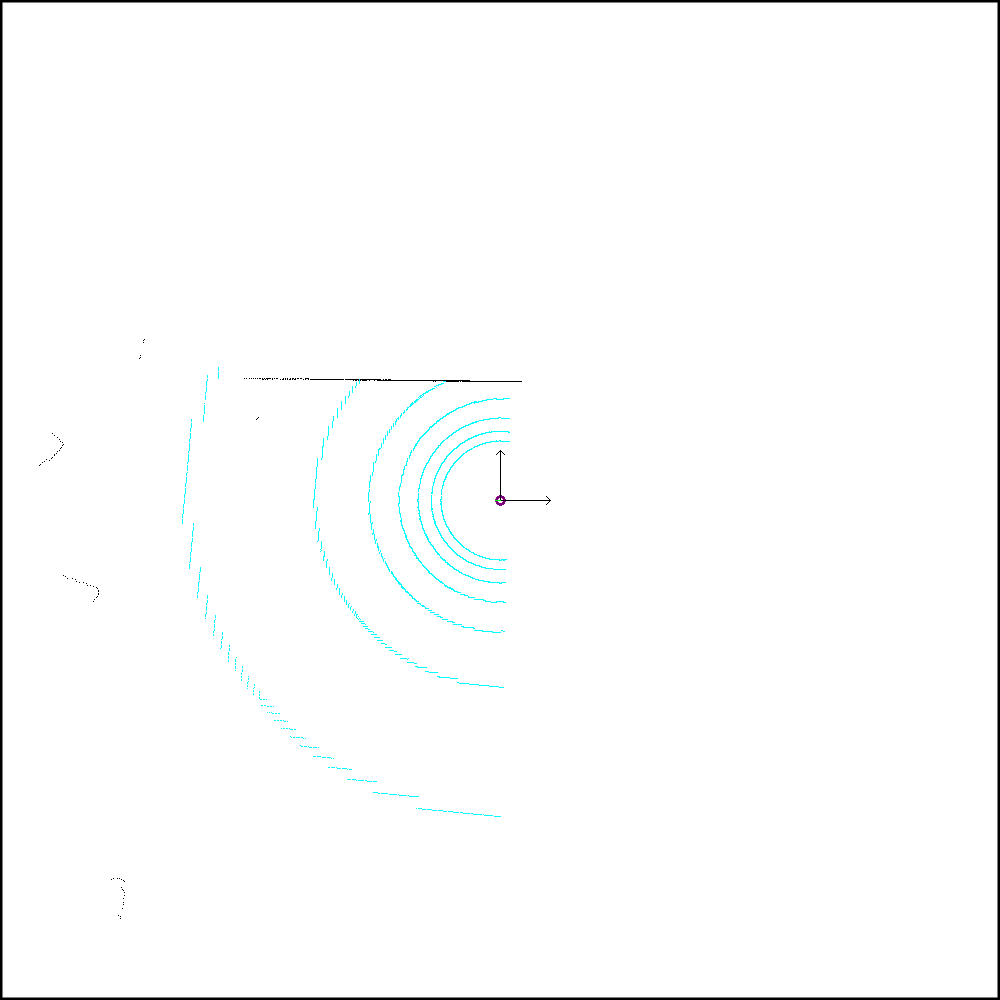
\includegraphics[width=\textwidth]{bilder/alg/img100001_r.png}
        Timestep 1
    \end{minipage}% <- sonst wird hier ein Leerzeichen eingefügt
    \hfill
    \begin{minipage}[t]{0.49\textwidth}
        \centering
	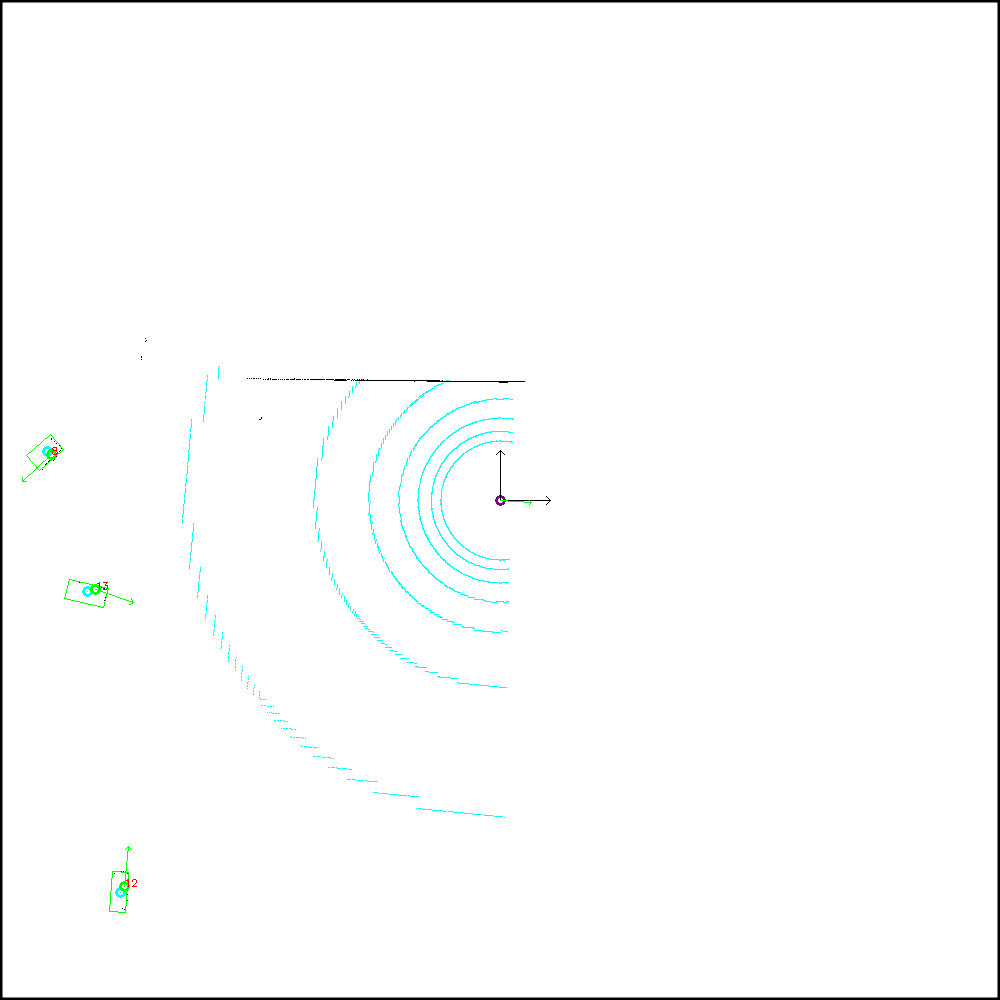
\includegraphics[width=\textwidth]{bilder/alg/img100002_r.png}
        Timestep 2
    \end{minipage}
    \label{detection_performance}
\end{figure}


Im zweiten Zeitschritt sehen wir das 3 objekte erkannt werden. Bei allen dieser Objekte handelt es sich um Fahrzeuge. Das Fahrzeug in der unteren in linken seite hat dabei eine Entfernung von 68 metern zum Testfahrzeug und wurde korrekt erkannt und klassifizierfiziert.
Die Farbe der Boxen stellt dabei den Typ der Klassizierung dar, grüne boxen sind Fahrzeuge, blaue boxen Radfahrer.

Die maximlae entfernung bei der Fahrzeug vollständig erkannt werden kann wurd in im Rahmen der Simulation mit nahe 95m bestimmt. was durch die Reichweite des Sensors limitiert
wird. Ob das Fahrzeug dabei korrekt Klassifiziert, hängt von der Ausrichtung des Fahrzeuges ab. Bewegt sich das Fahreug gerade auf das Testfahrzeug zu kann nur die Front des Fahrzeuges gesehen werden.
Das fürt dazu, dass das Fahrzeug eine Falsche größe hat, und als Radfahrer oder Fußgänger erkannt wird. Da für die Berecnung der Größe ein Historamm herangezogen wird, hat diese Falsche Klassifisierung
solange bestand, bis das Historamm auf die richtige größe konvergiert.

Sehen wir uns den zweiten Zeiitschritt genauer an \cref{detection_performance2} können wir ekennen, das sowohl Fußgänger und Radfahrer, obwohl in den Daten sichtbar (Rote Boxen), nicht erkannt werden.
Dies ist darin begründet, dass diese den $minPts$ Threshold des \ac{DBSCAN} nicht überschreiten. Dies ist erst der Fall wenn diese sich näher am Testfahrzeug befinden, genauer innerhalb des 6. Messlayers des Sensors (ca 23m)

\begin{figure}[!htb]
  \caption{Detection Distance Performance Pedestians/Cyclists} 
  \centering
  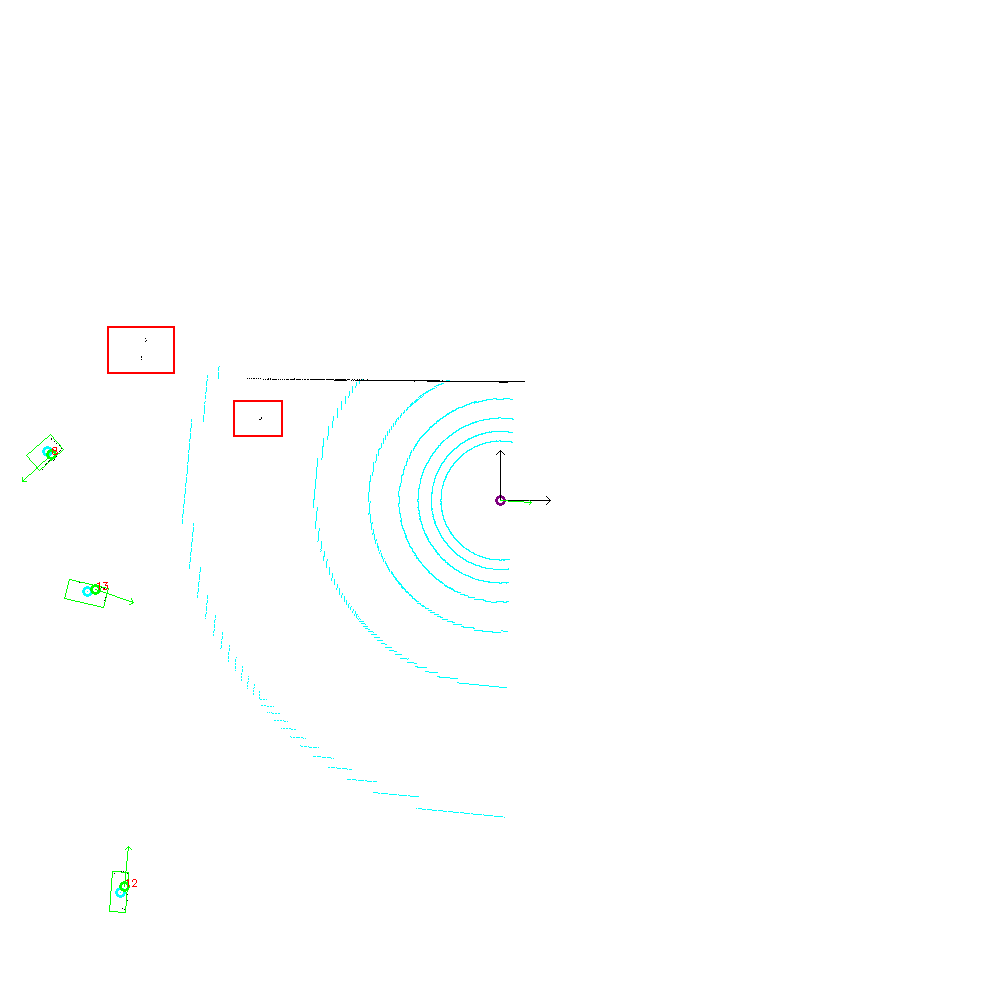
\includegraphics[width=\textwidth]{bilder/alg/img100002_m.png}
 \label{detection_performance2}
\end{figure}



\subsection{Measurements Performance}

In diesen abschnitt evaluieren wir die qualität in der Simulation messbaren größen, Geschwindigkeit und Position der Objekte.
Dazu wurde ein während der Simulation ständig sichtbares Fahzzeug ausgewählt. Dies ist das einzige Fahrzeug, was sich nicht ständig innerhalb des Kreisverkehres befindet, sondern in diesen einfährt und wieder verlässt.
Der Pfad des Fahhrzeuges ist in \cref{car_path1} zu sehen. Der Fehler der Position wurde dabei aus der euklidischen distanz der Position innerhalb der Simulation und der erkannten Position berechnet.

\begin{figure}[!htb]
  \caption{Car Path} 
  \centering
  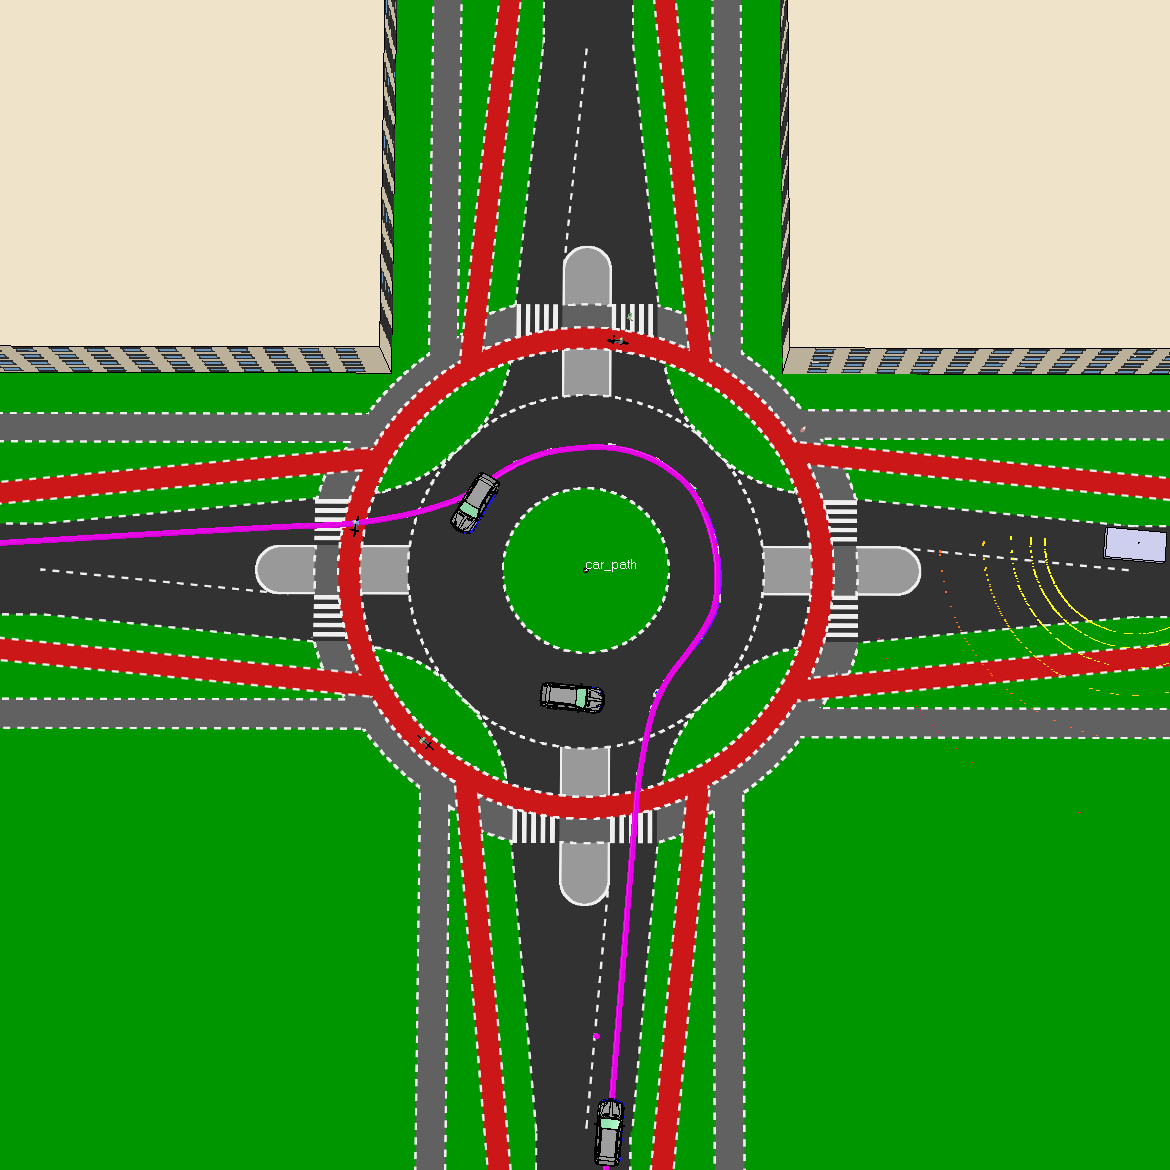
\includegraphics[width=\textwidth]{bilder/car_path.png}
 \label{car_path1}
\end{figure}

\subsubsection{Position Error}

Betrachten wir nun den Fehler der Position über die Zeit \cref{car_pos_err}. Die Legende der Abbildung ist die jeweilige ID des Trackings zu erkennen.
Es ist ersichtlich, das das dem Fahrzeug zwei verschiedene ID's zugeordnet wurden, was bedeutet, das das Tracking das Fahrzeug einmal verloren hat.

\begin{figure}[!htb]
  \caption{Car Position Error} 
  \centering
  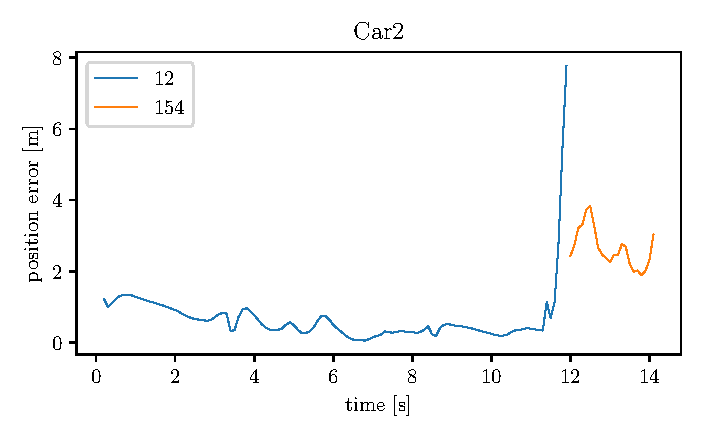
\includegraphics[width=\textwidth]{bilder/Car2_pos_err.pdf}
 \label{car_pos_err}
\end{figure}
Betrachten wir die Daten genauer, sehen wir, dass die Position in dem Bereich, in dem das Fahhzeug stabil erkannt werden kann einen Fehler, von rund 0.8 metern aufweißt.
in dem Moment in dem Das Fahrzeug nicht mehr getrackt werden kann, steigt der fehler rasant an, bis das Tracking das Objekt als ungütig erkennt.
Weiterhin ist zu erkennen, das nachdem dem Fahrzeug eine neue ID zugewiesen wurde, der Positionsfehler insgeammt höher ist.

Die Ursache des größen Fehlers in der Position liegt unter anderem im verhalten des Kalman Filters. Wie in \cref{kalman_error} zu sehen
befindet sich die Position des Filters (hellblau) beri eine Fahrzeug innerhalb des Kreisverkehres immer etwas ausßerhalb des Rechteckmittelpunktes.
Dies ist darin begründet, das dr Filter mit einem \ac{CTRV} Modell arbeitet, was nicht ganz das Verhalten der Fahrzeuge wiederspiegelt.
Denn diese Bewegen sich nicht in die Richtung ihrer aktuellen ausrichtung, sondern annährend iherer  Fahrdynamik.

\begin{figure}[!htb]
  \caption{Car Position Error} 
  \centering
  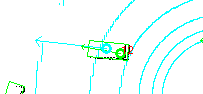
\includegraphics[width=0.5\textwidth]{bilder/kalman.png}
 \label{kalman_error}
\end{figure}



Sehen wir uns im Folgenden in \cref{lost} an, warum das Fahrzeug veroren ging und der Positionfehler gestiegen ist.

\begin{figure}[htb]
  \caption{Tracking Error} 
    \centering
    \begin{minipage}[t]{\textwidth}
        \centering
        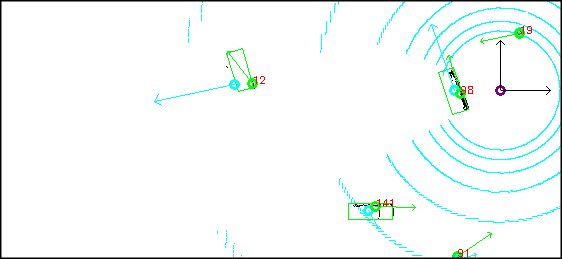
\includegraphics[width=\textwidth]{bilder/alg/lost.png}
    \end{minipage}% <- sonst wird hier ein Leerzeichen eingefügt
    \\
    \begin{minipage}[t]{\textwidth}
        \centering
	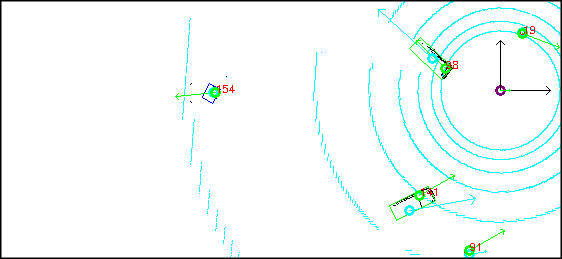
\includegraphics[width=\textwidth]{bilder/alg/redetect.png}
    \end{minipage}
    \label{lost}
\end{figure}

Darin ist zu erkennen, dass das Objekt  zum Großtei durch Objekt 98 verdeckt wird,  dadurch ist sowohl die Position als auch die Ausrichtung des Objektes Fehlerhaft.
Der Kalman Filter (hellblauer punkt und pfeil) behält jedoch grob die Bewegungsrichtung bei. Der Confidence wert des onjektes scheit jedoch nichtr auszureichen um das Objekt bis zu dem
Zeitpunkt zurückzuverfolgen, bis dieses wieder sichtbar ist. Im zweite teil der Abbildung sehen wird, das das Fahrzeug einige Zeitschritte später wieder erkannt werden kann.
Da wir das Fahrzeug nun niur von hinten sehen können. Wird die Größe des Fahrzeuges Falsch erkannt. Dadurch wird dieses als Fahrrad klassifiziert und da die Position
des Fahrzeiges aus dem Mittelpunkt des Rechteckes berechnet wird führt dies zu einem Systematischen Fehler. Wir sehen auch, das wir im vordern Bereich des Fahrzeuges Messerte bekommen.
Dies sind die Räder des Fahrzeuges, die wir aufgrund des Steilen Messwinkels sehen können. Da die Distanz zum Rest des Objektes allerdings zu groß ist, werden diese nicht 
zum Objekt hinzugefügt.

Da die Reine bertrachtung des Positionsfehlers nicht serh ausssagekrftig ist, sehen wir uns nun den Fahler in abhängigkeit von der Entfernung zu Testfahrzeug an.

\begin{figure}[!htb]
  \caption{Car Position Error / Distance} 
  \centering
  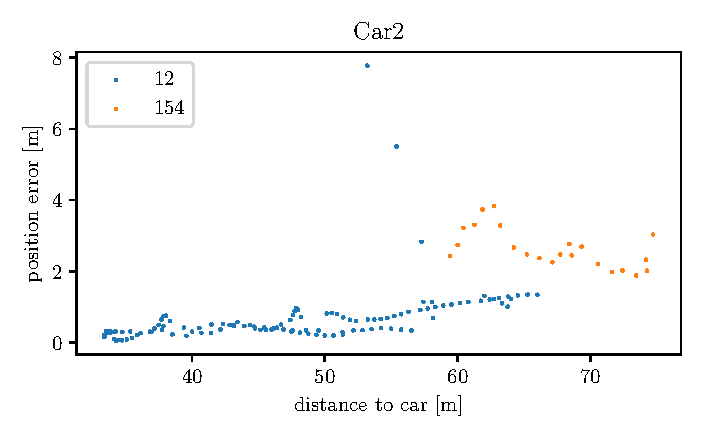
\includegraphics[width=\textwidth]{bilder/Car2_pos_err_dist.pdf}
 \label{car_pos_err}
\end{figure}

Lassen wir den Positionsfehler von Objekt 154 außer acht, sehen wir, dass der Fahler mit der Entfernung konstant zunimmt. Was auf dem ersten Blick intutiv logisch erscheint,
erinnern wir uns jedoch an \cref{detection_performance2} zuück, sehen wird das Das Objekt innherlab der Messdaten auch bei grlößen entfernungeb korrekt erkannt wird.
Das Konstate ansteigen der Position ist stadtdessen in einer limitierung der Simulationssoftware zu suchen.

\begin{figure}[!htb]
  \caption{Simualtion Sensor Resolution} 
  \centering
  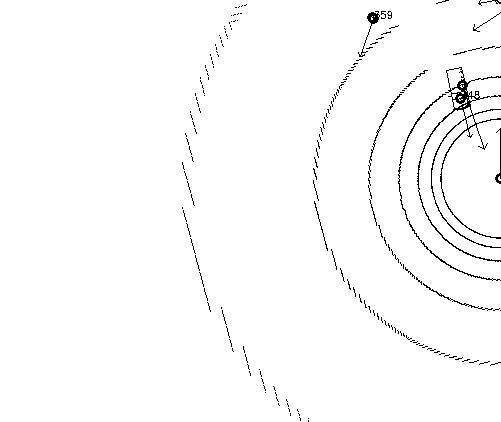
\includegraphics[width=0.5\textwidth]{bilder/sen_err.png}
 \label{sen_res}
\end{figure}

Auf \cref{sen_res} gut zu sehen, ist das die Auflösung der Sensor messwerte mit zunehmender Entfernung immer weiter abnimmt, was zu einer Rasterung der Messkreise führt. Dies ist darin begründet,
das dieser mit hilfe von OpenGL simuliert wird, welches mit fixed point arithmetic arbeitet. Im letzten im bild ersichtlichen Messlayer des Sensors beträgt die 
Auflösung des Sensors nur noch 2m. Diese Eigenschaft tritt offensichtlich nicht mit dem Realensensort auf. Leider Wurden keine geeigenten messdaten für den realen Velodyn sensor aufgenommnen.
die Eine evaluierung dahingehend ermöglichen

.
\subsubsection{Speed}

Das für die bewältiging des Simulationsszenarios abgesehen von der Position auch die Geschwindigkeit der Objekte besonders wichtig ist, vergleichen wir im
folgenden die Geschwindigkeit der erkannnten Objekte mit den realen werten in der Simulation. Dazu sind in \cref{car2_speed} die Messwerte
grafisch dargestellt. Der Graph Car2 stellt dabei die Idealen werte aus der Simualtion dar.


\begin{figure}[!htb]
  \caption{Car2 Speed} 
  \centering
  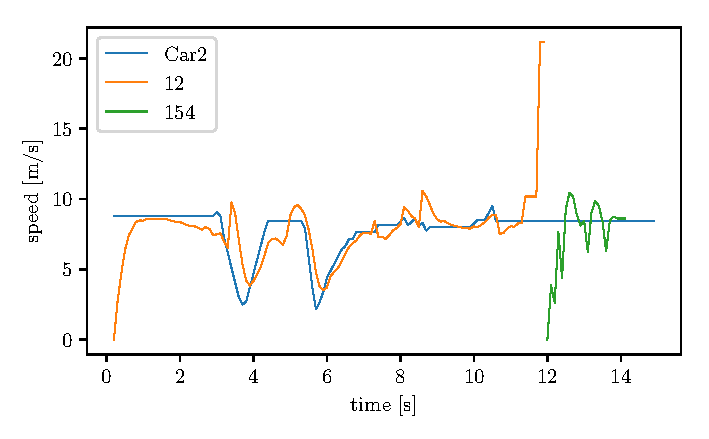
\includegraphics[width=\textwidth]{bilder/Car2_speed.pdf}
 \label{car2_speed}
\end{figure}

Da die geschwindigkeit der Objekte aus der Position abgeleitet ist, ist sie im initalen Zeitschritt null was gut in der Abbildung zu erkennen ist.
Weiterhin fällt ausßerdem auf, dass die Messwerte den idealen werten zwar folgen, jedoch verzögert sind. Dies lässt sich ebenfalls auf die Ableitung der Geschwindigkeit
aus der Positionsänderung zurückführen.  Liegt jedoch auch am von Kalman Filter verwendetetn \ac{CTRV} Model, welchen von einer konstanten gewschwindigkeit ausgeht.
Aus diesem Grund wirkt der Kalman Filter hier wie ein einfacher Tiefpass und verzögert die Werte zusätlich. Außreißer treten jedoch auch hier auf, wenn Tracking im begriff ist, das Objekt zu verlieren.

Beterachten wir ein andrers Fahrzeug, mit einer konstaten Geschwindigekeit in \cref{car0_speed}. 
\begin{figure}[!htb]
  \caption{Car2 Speed} 
  \centering
  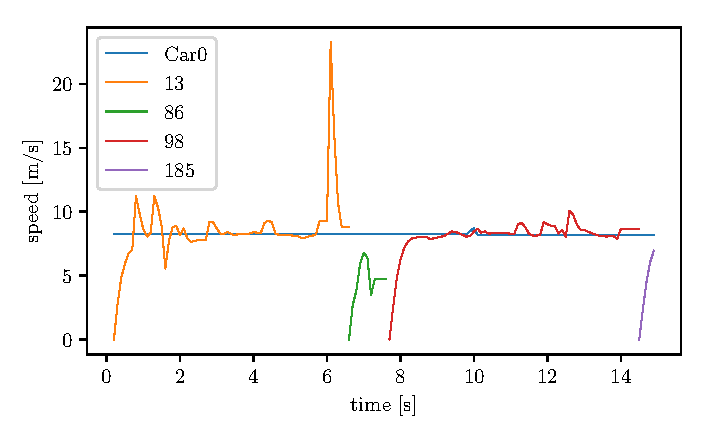
\includegraphics[width=\textwidth]{bilder/Car0_speed.pdf}
 \label{car0_speed}
\end{figure}
Hier ist gut zu erkennen, dass sich die werte nach einer kurzen einschwingzeit stets nahe am echte wert befinden. Die Stärkern abweichungen in den ersten drei Sekunden sidn auf eine Instabile
erkennung des Fahrzeiges aufgrund eines Ungünstigen winkels des Fahrzeuges zum realen Fahrzeug zurückzuführen.  Besoders im Zeitraum von Sekunde 8 bis 14 ist jedoch immer eine optimale
erkennung des Fahrzeuges gegeben und die Messwerte haben nur eine geringe Abweichung.


\subsubsection{Scenario Handling}
Im folgen werten wir das Simulationsscenario an sich aus, idem wir die beiden krittischen Situationen das einfahren und ausfahren des testfahrzeuges aus dem Kreisverkehr 
innerhalb der Objektdetection Ansehen.


Bild mit Rotationsproblemen\\


Bilder Classifizierung der Objekte (Radfahrer falsch etc...)\\

Bilder Erfolgreiche erkennungen.\\

Digramm komplettausfall erkennung (ab welcher entfernung)\\

\section{Real Measurements}

Probleme mit Noise von umgebeung\\

Probleme Segementierung (mit diagramm ground detection (x,y,z wert des Normalenverktors))\\

Probleme mit verschmelzen von objekten\\


\section{Performance}

Benchmark und Profilingchart einfügen.\\




\chapter{Conclusions}
Kann in mehrere Unterkapitel gegliedert werden\\\\
Greift Thesen oder Fragestellungen aus der Einleitung wieder auf\\\\
Fasst die Arbeit knapp und prägnant zusammen\\\\
Ordnet die Ergebnisse in Gesamtzusammenhänge ein\\\\
Zieht Schlussfolgerungen aus den erarbeiteten Ergebnissen\\\\
Kann auch eigene Bewertungen oder Meinungen enthalten\\\\
Gibt eine Ausblick auf mögliche Konsequenzen oder notwendige weitere zu lösende Probleme
\chapter{Future Work}

\printbibliography

\end{document}          
